\documentclass{article}
\input{new_commands}

% if you need to pass options to natbib, use, e.g.:
\PassOptionsToPackage{numbers, sort, compress}{natbib}
% before loading neurips_2024


% ready for submission
%\usepackage{neurips_2024}


% to compile a preprint version, e.g., for submission to arXiv, add add the
% [preprint] option:
\usepackage[preprint]{neurips_2024}

% \usepackage{iclr2026_conference, times}
% \usepackage{iclr2026_arxiv}
% Optional math commands from https://github.com/goodfeli/dlbook_notation.
\input{math_commands.tex}


\usepackage[utf8]{inputenc} % allow utf-8 input
\usepackage[T1]{fontenc}    % use 8-bit T1 fonts
\usepackage{hyperref}       % hyperlinks
\usepackage{url}            % simple URL typesetting
\usepackage{booktabs}       % professional-quality tables
\usepackage{amsfonts}       % blackboard math symbols
\usepackage{nicefrac}       % compact symbols for 1/2, etc.
\usepackage{microtype}      % microtypography
\usepackage{xcolor}         % colors

%%%

\usepackage{subcaption}
\usepackage{graphicx}
\usepackage{multirow}
\usepackage{amsmath,amssymb,amsfonts}
\usepackage{amsthm}
\usepackage{mathrsfs}
% \usepackage{xcolor}
\usepackage[dvipsnames]{xcolor}
\usepackage{textcomp}
\usepackage{manyfoot}
\usepackage{booktabs}
\usepackage{algorithm}
\usepackage{algorithmicx}
\usepackage{algpseudocode}
\usepackage{listings}
\usepackage{diagbox}
\usepackage{wrapfig}

\graphicspath{{figs}}

%%% TIKZ %%%

\usepackage{tikz}
\usetikzlibrary{arrows.meta,calc,fit,positioning,backgrounds}

\definecolor{ff}{RGB}{193,231,247}   % FeedForward
\definecolor{sa}{RGB}{255,225,188}  % Self-Attention
\definecolor{ln}{RGB}{242,244,192}   % LayerNorm

\definecolor{plotBlue}{RGB}{31,119,180}  % as in matplotlib
\definecolor{plotOrange}{RGB}{255,127,14}  % as in matplotlib

%%%%%%%%%%%%

\newtheorem{theorem}{Theorem} % continuous numbers
%%\newtheorem{theorem}{Theorem}[section] % sectionwise numbers
%% optional argument [theorem] produces theorem numbering sequence instead of independent numbers for Proposition
% \newtheorem{proposition}[theorem]{Proposition}% 
%%\newtheorem{proposition}{Proposition} % to get separate numbers for theorem and proposition etc.

\newtheorem{example}{Example}
\newtheorem{remark}{Remark}

\newtheorem{definition}{Definition}
\newtheorem{assumption}{Assumption}

\newtheorem{lemma}{Lemma}
\newtheorem{proposition}{Proposition}

\newtheorem{property}{Property}

%%%


\title{Closing the Curvature Gap: Full Transformer Hessians and Their Implications for Scaling Laws}


% The \author macro works with any number of authors. There are two commands
% used to separate the names and addresses of multiple authors: \And and \AND.
%
% Using \And between authors leaves it to LaTeX to determine where to break the
% lines. Using \AND forces a line break at that point. So, if LaTeX puts 3 of 4
% authors names on the first line, and the last on the second line, try using
% \AND instead of \And before the third author name.


\author{
  Egor Petrov\\
  Yandex, BRAIn Lab\\
  \texttt{moderntalker@yandex-team.ru}\\
  \And
  Nikita Kiselev\\
  Independent\\
  \texttt{bashmak22@gmail.com}\\
  \And
  Vladislav Meshkov\\
  Independent\\
  \texttt{vladmeshkov160@gmail.com}
  \And 
  Andrey Grabovoy\\
  Moscow State University\\
  \texttt{andriy.graboviy@gmail.com}\\
}


\begin{document}


\maketitle

\begin{abstract}
    The lack of theoretical results for Layer Normalization and feedforward Hessians has left a gap in the study of Transformer optimization landscapes. We address this by deriving explicit second-order expressions for these components, thereby completing the Hessian characterization of full Transformer blocks. Our results generalize prior self-attention analyses and yield estimations for the role of each sublayer in curvature propagation. We demonstrate how these Hessian structures inform both convergence dynamics and the empirical scaling laws governing large-model performance. Further, we propose a Taylor-expansion–based framework for analyzing loss differences to quantify convergence trajectories. By extending Hessian theory to the full Transformer architecture, this work establishes a new foundation for theoretical and empirical investigations of optimization in large-scale deep learning.
\end{abstract}

\textbf{Keywords:} Transformer Hessians, Layer Normalization, Scaling laws, Convergence dynamics, Loss landscape, Optimization geometry.

\section{Introduction}\label{sec:intro}

\begin{figure}[h]
    \centering
    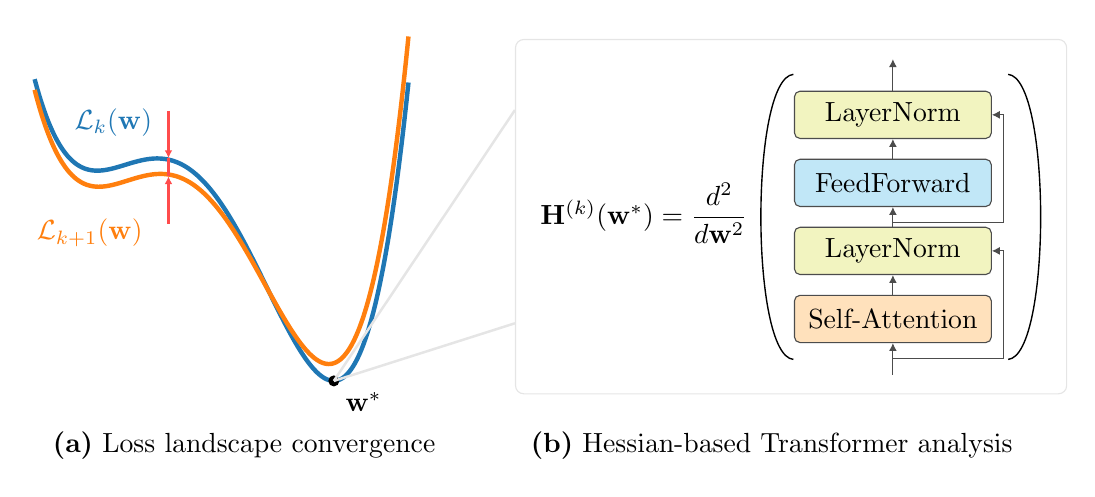
\begin{tikzpicture}[
      >=Latex,
      lossA/.style={ultra thick, plotBlue},
      lossB/.style={ultra thick, plotOrange},
      dot/.style={circle, inner sep=1.3pt, fill=black},
      layer/.style={rounded corners=2pt, draw=black!70, minimum width=2.5cm, minimum height=6mm, align=center},
      layerLN/.style={layer, fill=ln},
      layerSA/.style={layer, fill=sa},
      layerFF/.style={layer, fill=ff}
    ]
    
    \tikzset{>={Latex[length=1mm,width=1mm]}}
    
    % -------- LEFT PANEL (no axes) --------
    \node[minimum width=7.0cm, minimum height=5.0cm, anchor=south west, inner sep=0] (L) at (0,0) {};
    
    \begin{scope}[shift={(0.6,1.2)}]
      % Две устойчивые quartic-кривые
      \def\LossA#1{ 0.2*((#1 - 0.1)^4-5*(#1)^3+6*(#1)^2-(#1)) + 2 }
      \def\LossB#1{ 0.2*((#1 - 0.1)^4-5*(#1-0.02)^3+6*(#1 - 0.02)^2-(#1)) + 1.8 }
    
      \draw[lossA, domain=-0.7:4.05, samples=160, smooth]
        plot (\x, {\LossA{\x}});
      \draw[lossB, domain=-0.7:4.05, samples=160, smooth]
        plot (\x, {\LossB{\x}});
    
      % минимум w*
      \coordinate (wstar) at (3.1, { \LossA{3.1} });
      \fill (wstar) circle (2pt);
      \node[below right=1pt of wstar] {$\mathbf{w}^*$};
    \end{scope}
    
    \node[text=plotBlue] (Lk) at (0.9, 3.8) {$\mathcal{L}_{k}(\mathbf{w})$};
    \node[text=plotOrange] (Lkp1) at (0.6, 2.4) {$\mathcal{L}_{k+1}(\mathbf{w})$};

    % точки верха/низа
    % \coordinate (gapTop) at (1.6,{ \LossA{1.6} });
    % \coordinate (gapBot) at (1.6,{ \LossB{1.6} });

    \coordinate (gapTop) at (1.6,3.35);
    \coordinate (gapBot) at (1.6,3.12);
    
    % вертикальный отрезок (щель)
    \draw[red!70, very thick] (gapBot) -- (gapTop);
    
    % стрелки, «подпирающие» щель
    \draw[red!70, ->, thick] ([yshift=0.6cm]gapTop) -- (gapTop);
    \draw[red!70, ->, thick] ([yshift=-0.6cm]gapBot) -- (gapBot);
    
    \node at ($(L.south)!0.5!(L.south east)+(-2.7,-0.3)$) {\textbf{(a)}~Loss landscape convergence};
    
    % -------- RIGHT PANEL --------
    \coordinate (R0) at (6,0.35);
    \node[draw=gray!20, rounded corners=3pt, minimum width=7cm, minimum height=4.5cm,
          anchor=south west, fill=white] (R) at (R0) {};
    
    % серые zoom-линии
    \draw[gray!20, line width=0.9pt] (wstar) -- ($(R.west)!0.6!(R.north west)$);
    \draw[gray!20, line width=0.9pt] (wstar) -- ($(R.west)!0.6!(R.south west)$);
    
    % внутри правой панели: H^(k)(w*) = d^2/dw^2 ( [schema] )
    \begin{scope}[shift={(6.2,0.45)}]
      % левая часть формулы
      \node[anchor=west] (Hleft) at (0,2.2)
        {$\mathbf{H}^{(k)}(\mathbf{w}^*) = \dfrac{d^2}{d \mathbf{w}^2}$};
    
      % стек слоёв
      \node[layerLN] (ln2) at (4.6,3.45) {LayerNorm};
      \node[layerFF, below=2.5mm of ln2] (ff) {FeedForward};
      \node[layerLN, below=2.5mm of ff] (ln1) {LayerNorm};
      \node[layerSA, below=2.5mm of ln1] (sa) {Self-Attention};

      \coordinate (sa_south_east) at ($(sa.south)+(14mm,-2mm)$);
      \coordinate (ff_south_east) at ($(ff.south)+(14mm,-2mm)$);
      
      \draw[->, black!70] ($(sa.south)+(0mm,-4mm)$) -- (sa);
      \draw[->, black!70] (sa) -- (ln1);
      \draw[->, black!70] (ln1) -- (ff);
      \draw[->, black!70] (ff) -- (ln2);
      \draw[->, black!70] (ln2) -- ($(ln2.north)+(0mm,4mm)$);

      \draw[->, black!70] ($(sa.south)+(0mm,-2mm)$) -- (sa_south_east) |- ($(ln1.east)+(0mm,0mm)$);
      \draw[->, black!70] ($(ff.south)+(0mm,-2mm)$) -- (ff_south_east) |- ($(ln2.east)+(0mm,0mm)$);
    
      % коробка, вокруг которой рисуем скобки — и чтобы не «уехало»
      \node[inner sep=0mm, fit=(sa) (ln1) (ff) (ln2)] (stackbox) {};
    
      % скобки, точно «обнимающие» стек
      \draw[line width=0.5pt]
        ($(stackbox.north west)+(0,0.20)$)
          .. controls +(-0.55,-0.05) and +(-0.55,0.05) ..
        ($(stackbox.south west)+(0,-0.2)$);
      \draw[line width=0.5pt]
        ($(stackbox.north east)+(+0.2,0.2)$)
          .. controls +(0.55,-0.05) and +(0.55,0.05) ..
        ($(stackbox.south east)+(+0.2,-0.2)$);
    
      % аккуратный зазор между формулой и скобкой
      \node at ($(Hleft.east)!0.0!(Hleft.east)$) {}; % якорь (оставляет фиксированный промежуток)
    \end{scope}
    
    \node at ($(R.south)!0.5!(R.south east)+(-2,-0.65)$) {\textbf{(b)}~Hessian-based Transformer analysis};
    
    \end{tikzpicture}
    \caption{\textbf{Overview of our observations.} Part (a) shows the loss function landscape, which is a
surface in the parameters space, and how it changes as the dataset size increases. Part (b) shows the schematic view of a proposed method~--- carry out an analysis of a Transformer's Hessian, which greatly impacts on a loss landscape convergence, leading to a sample size determination framework.}
    \label{fig:introduction}
\end{figure}

Transformers \cite{vaswani2017attention} have revolutionized deep learning, achieving state-of-the-art performance across natural language processing \cite{devlin2019bert, brown2020language}, computer vision \cite{dosovitskiy2021image, wu2020visualtransformer}, 
% and scientific applications \cite{jumper2021highly, moreno2024medicalfewshot}. % [CHANGE: Added citations to highlight broad applicability of Transformers]. 
Their empirical success is underpinned by predictable improvements in model quality with increased dataset size, as described by neural scaling laws \cite{kaplan2020scaling}; \cite{hoffmann2022training, bahri2024explainingscalinglaws}. However, many domains, such as medical imaging \cite{moreno2024medicalfewshot} and scientific discovery \cite{jumper2021highly}, face severe data constraints where acquiring additional samples is costly or infeasible \cite{chen2025dataefficientgeneralizationzeroshotcomposed}. % [CHANGE: Added recent citation and emphasized data constraints]. 
This tension necessitates a rigorous theoretical understanding of how dataset size shapes the optimization landscape and influences training dynamics.

Existing theoretical analyses of Transformer optimization landscapes are incomplete. While recent studies have derived Hessian expressions for self-attention mechanisms \cite{ormaniec2024attentionhessian, zhang2024why}, the full Transformer block—including LayerNorm and feed-forward networks (FFNs)—lacks a comprehensive theoretical characterization \cite{noci2022signalpropagationtransformerstheoretical, zhang2025understanding}. % [CHANGE: Added recent citations and clarified scope]. 
These components critically influence optimization dynamics, such as gradient flow and convergence rates \cite{noci2022signalpropagationtransformerstheoretical, unknown}, and generalization behavior \cite{zhang2025understandinggeneralizationincontextlearning, csordas-etal-2021-devil}. Without a complete curvature analysis, our understanding of Transformer training dynamics, convergence properties, and scaling behavior remains limited \cite{fort2019emergentpropertieslocalgeometry}.

In this work, we provide the first complete theoretical analysis of the Hessian for full Transformer blocks, extending beyond prior self-attention analyses \cite{ormaniec2024attentionhessian, zhang2024why} to include explicit second-order expressions for LayerNorm and FFNs.
% [CHANGE: Emphasized novelty and included recent citation]. 
Our analysis derives rigorous bounds on how the loss landscape evolves with dataset size, offering a novel framework for understanding landscape stabilization in Transformers. These results have implications for optimization challenges (e.g., vanishing gradients \cite{hochreiter1998vanishing}), scaling laws (e.g., compute-optimal training \cite{hoffmann2022training, kaplan2020scaling}), and critical batch size estimation \cite{mccandlish2018empirical, zhang2025how}. 
%[CHANGE: Added connections to optimization, scaling laws, and critical batch size with recent citations].

\textbf{Contributions.} Our main contributions are:
\begin{itemize}
    \item We derive the first full Hessian expressions for Transformer blocks, including explicit treatment of LayerNorm and FFNs, filling a critical gap in prior analyses.
    \item We establish theoretical bounds on the loss landscape’s evolution with dataset size, providing a rigorous framework for understanding landscape stabilization.
    \item We validate our theoretical predictions through experiments on Vision Transformers, demonstrating practical relevance across data regimes.
\end{itemize}

Our work bridges theoretical deep learning and practical Transformer deployment, enabling new insights into optimization difficulties, efficient scaling strategies, and future theoretical investigations of large-scale deep learning. % [CHANGE: Added citations to reinforce implications].

\textbf{Outline.} The rest of the paper is organized as follows. In Section  \ref{sec:rw}, we review related work, categorizing existing research into key topics and highlighting their main contributions. Section \ref{sec:prelim} introduces the notation and presents preliminary calculations essential for our analysis. In Section \ref{sec:method}, we derive theoretical bounds for the norm of the Hessian matrix and the norm of the difference between loss functions. Section \ref{sec:exp} provides an empirical study validating these theoretical results. Section \ref{sec:disc} discuss and summarize our findings, offering insights and conclusions. Additional experiments are in Appendix \ref{app:A} and proofs of theorems are included in Appendices \ref{app:properties}-\ref{app:additional_properties}.

\section{Related Work}\label{sec:rw}

\textbf{Geometry of Neural Network Loss Landscapes} Foundational studies characterize neural loss geometry via Hessians, including class-aligned high-curvature directions \cite{fort2019emergentpropertieslocalgeometry}, random-matrix perspectives on spectra and optimization \cite{pmlr-v70-pennington17a}, and connectivity and double-descent phenomena \cite{garipov2018losssurfacesmodeconnectivity, singh2022phenomenologydoubledescentfinitewidth, draxler2019essentiallynobarriers, nguyen2017losssurfacedeepwide}, with flattening observed at large learning rates \cite{wang2023instabilitieslargelearningrate}. Our work complements this line by showing how curvature of Transformer blocks changes with dataset size, providing explicit second-order bounds that formalize landscape stabilization under data growth. This links classical geometric insights to a data-scaling axis that was previously qualitative.

\textbf{Hessian-Based Analysis and Generalization} Prior Hessian analyses for fully connected and convolutional networks reveal spectral structure and low effective rank with implications for convergence and smoothness \cite{kiselev2024unraveling, meshkov2024convnets}. We extend these ideas to Transformers by deriving explicit LayerNorm/FFN second derivatives and blockwise spectral-norm bounds, thereby closing a missing piece in second-order geometry for this architecture.

\textbf{Loss Landscapes in Transformers} While Transformers \cite{vaswani2017attention} have inspired curvature analyses focused on attention \cite{ormaniec2024attentionhessian} and studies of sample complexity, generalization, and stagewise dynamics \cite{li2023theoreticalunderstandingshallowvision, zhang2025understandinggeneralizationincontextlearning, anonymous2024stagewisedevelopmenttransformers}, a full-block second-order treatment has remained incomplete. We provide the missing LayerNorm/FFN Hessians and assemble a complete blockwise Hessian for a Transformer layer, aligning theory with empirical curvature structure. This enables a principled account of how Transformer curvature evolves with data and training.

\textbf{Dataset Size and Loss Landscape Convergence} Work on compute-optimal scaling and sample-related flatness highlights the importance of balancing data and model size \cite{hoffmann2022training, wu2017towards}, and visualization tools hint at stabilization thresholds without theory \cite{xie2024losslens}. Building on Hessian frameworks from other architectures \cite{kiselev2024unraveling, meshkov2024convnets} and attention derivatives \cite{ormaniec2024attentionhessian}, we derive a second-order bound that decays as $1/k$. This yields actionable diagnostics for curvature-aware training and data budgeting in Transformers.

\section{Preliminaries}\label{sec:prelim}

We adopt row-wise vectorization \(\mathrm{vec}_r(\cdot)\) from \cite{ormaniec2024attentionhessian, noci2022signalpropagationtransformerstheoretical}. For a matrix-valued function \(\mathbf{N}: \mathbb{R}^{p \times q} \to \mathbb{R}^{n \times d}\) differentiable w.r.t.\ weight matrices \(\mathbf{W}_i \in \mathbb{R}^{p_i \times q_i}\) and \(\mathbf{W}_j \in \mathbb{R}^{p_j \times q_j}\), the Jacobian is \(\frac{\partial \mathbf{N}}{\partial \mathbf{W}_i} := \frac{\partial \mathrm{vec}_r(\mathbf{N})}{\partial \mathrm{vec}_r(\mathbf{W}_i)^\top} \in \mathbb{R}^{n d \times p_i q_i}\), and the Hessian block is \(\frac{\partial^2 \mathbf{N}}{\partial \mathbf{W}_i \partial \mathbf{W}_j} := \frac{\partial \mathrm{vec}_r(\frac{\partial \mathbf{N}}{\partial \mathbf{W}_i})}{\partial \mathrm{vec}_r(\mathbf{W}_j)^\top} \in \mathbb{R}^{(n d \cdot p_i q_i) \times p_j q_j}\). Key properties (e.g., for products, Kronecker, inverses, Hadamard powers) are detailed in Appendix~\ref{app:properties}.

Let \(f_{\mathbf{w}}(\cdot)\) denote a neural network (here, a Self-Attention layer or full Transformer block) with parameters \(\mathbf{w} \in \Omega\). Given a twice-differentiable loss \(l(\cdot, \cdot)\), the per-sample loss is \(l_i(\mathbf{w}) := l(f_{\mathbf{w}}(\mathbf{x}_i), \mathbf{y}_i)\). The empirical loss over \( L = k\) samples is \(\mathcal{L}_k(\mathbf{w}) = \frac{1}{k} \sum_{i=1}^k l_i(\mathbf{w})\), with Hessian \(\mathbf{H}^{(k)}(\mathbf{w}) = \frac{1}{k} \sum_{i=1}^k \nabla^2_{\mathbf{w}} l_i(\mathbf{w})\).

\begin{assumption} \label{as:zero_grad}
At local minimum \(\mathbf{w}^*\), \(\nabla \mathcal{L}_{k-1}(\mathbf{w}^*) = \nabla \mathcal{L}_k(\mathbf{w}^*) = 0\).
\end{assumption}
Our study on the feasibility of this assumption is in Appendix \ref{app:exp_assumption_check}.

Consider input embeddings \(\mathbf{X} \in \mathbb{R}^{L \times d_V}\). A single-head Self-Attention layer outputs
\begin{equation} \label{eq:self_attention}
    \mathbf{F}(\mathbf{X}) = \mathbf{A}(\mathbf{X}) \mathbf{X} \mathbf{W}_V,
\end{equation}
where \(\mathbf{A}(\mathbf{X}) = \softmax\left( \frac{\mathbf{X} \mathbf{W}_Q \mathbf{W}_K^\top \mathbf{X}^\top}{\sqrt{d_K}} \right)\), and \(\mathbf{W}_Q, \mathbf{W}_K \in \mathbb{R}^{d_V \times d_K}\), \(\mathbf{W}_V \in \mathbb{R}^{d_V \times d_V}\). 

Full Transformer block is:
\begin{align}
\text{LayerNorm}\Big(\mathbf{\text{LayerNorm}(\mathbf{X} + \mathbf{F}(\mathbf{X}))} + \mathrm{FFN}(\mathbf{\text{LayerNorm}(\mathbf{X} + \mathbf{F}(\mathbf{X}))})\Big)
\end{align}
where \(\mathrm{FFN}(\cdot)\) is a fully connected block with a non-linear activation within it. LayerNorm for an input matrix $\mathbf{U} \in \mathbb{R}^{m \times n}$ is \(\text{LayerNorm}(\mathbf{U})_{i,j} = \gamma_j \frac{\mathbf{U}_{i,j} - \mu_i}{\sqrt{\sigma_i^2}} + \mathbf{\beta}_j\), where $\mu_i = \frac{1}{m} \sum_{j=1}^m \mathbf{U}_{i,j}, \quad \sigma_i^2 = \frac{1}{m} \sum_{j=1}^m (\mathbf{U}_{i,j} - \mu_i)^2$. More details on a transformer block are in Section \ref{subsec:hessian_transformer_block}.
\begin{assumption} \label{as:non_zero_variance}
For input matrices to LayerNorm (e.g., \(\mathbf{X} + \mathbf{F}(\mathbf{X})\), \(\mathbf{Y} + \mathrm{FFN}(\mathbf{Y})\)), the per-row variances satisfy \(\min_i \sigma_i^2 > 0\).
\end{assumption}
It's a technical assumption for the proof part simplification and numerical stability. The same effect can be achieved by adding some positive constant to the denominator, but it makes calculations harder. In our case this assumption is required for $\mathbf{X} + \mathbf{F}(\mathbf{X})$ and $\mathbf{Y} + \text{FFN}(\mathbf{Y})$, defined in Transformer block \ref{eq:transformer}.

We use mean-squared error loss: \(l(\cdot, \textbf{Target}) = \frac{1}{L d_V} \|\cdot - \textbf{Target}\|_F^2\). Hessians decompose via Gauss-Newton: for composite \(\mathcal{L}_k \circ f_{\mathbf{w}}\),
\begin{equation} \label{eq:gauss_decomposition}
\frac{\partial^2 (\mathcal{L}_k \circ f_{\mathbf{w}})}{\partial \mathbf{W}_i \partial \mathbf{W}_j} = \frac{\partial f_{\mathbf{w}}}{\partial \mathbf{W}_i} (\cdot)^\top \frac{\partial^2 \mathcal{L}_k}{\partial f_{\mathbf{w}}^2} (f_{\mathbf{w}}(\cdot)) \frac{\partial f_{\mathbf{w}}}{\partial \mathbf{W}_j}(\cdot) + \left( \frac{\partial \mathcal{L}_k}{\partial f_{\mathbf{w}}} (f_{\mathbf{w}}(\cdot)) \otimes \mathbf{I}_{p_i q_i} \right) \frac{\partial^2 f_{\mathbf{w}}}{\partial \mathbf{W}_i \partial \mathbf{W}_j}(\cdot)
\end{equation}

% \section{Preliminaries}\label{sec:prelim}

% \subsection{General notation}

% In this section, we introduce the general notation used in the rest of the paper and the basic assumptions similar to \cite{kiselev2024unraveling}. Let $f_{\mathbf{w}}(\cdot)$
% be a neural network with a space of parameters ($\mathbf{w} \in \Omega$). In this study we cover both single Self-Attention layer and whole Transformer layer as $f_{\mathbf{w}}(\cdot)$. Let $l(\cdot, \cdot)$ be a given twice differentiable loss function (e.g. MSE, cross-entrophy) where first argument refers to neural network's
% result and the second argument refers to the true answer. 

% % To simplify, define: $$l_i(\mathbf{w}) := l(f_{\mathbf{w}}(x_i), \text{target}_i).$$

% % The empirical loss function for the sequence length $L = k$:
% % $$\mathcal{L}_k(\mathbf{w}) = \frac1k \sum\limits_1^k l_i(\mathbf{w}), \,\, \mathcal{L}(\mathbf{w}) := \mathcal{L}_m(\mathbf{w}).$$

% % Thus, the difference between losses for neighbouring length sequences is:
% % $$\mathcal{L}_{k}(\mathbf{w}) - \mathcal{L}_{k-1}(\mathbf{w}) = \frac{l_{k}(\mathbf{w}) - \mathcal{L}_{k-1}(\mathbf{w})}{k}.$$

% %   The Hessian of \(\mathcal{L}_{k}(\mathbf{w})\) is:
% %   \[
% %   \mathbf{H}^{(k)}(\mathbf{w}) = \nabla^2_{\mathbf{w}} \mathcal{L}_{k}(\mathbf{w}) = \frac{1}{k} \sum_{i=1}^k \nabla^2_{\mathbf{w}} l_i(\mathbf{w}).
% %   \]

% \subsection{Assumptions}

% \begin{assumption} \label{as:zero_grad}
%   Let $\mathbf{w}^*$ be the local minimum of both $\mathcal{L}_{k-1}(\mathbf{w})$ and $\mathcal{L}_{k}(\mathbf{w})$.
%   Thus, $$\nabla \mathcal{L}_{k-1}(\mathbf{w}^*) = \nabla \mathcal{L}_{k}(\mathbf{w}^*) = 0.$$
% \end{assumption}

% This assumption allows us to explore the behavior and the geometry of the loss function landscape at only one point.

% \begin{assumption} \label{as:non_zero_variance}
%     For $\mathbf{X} \in \mathbb{R}^{m \times n}$, serving as an input matrix for the LayerNorm operation, we technically assume that $\min \limits_{i \in \{1 \dots n\}} ( \sigma_i^2 = \frac{1}{m} \sum_{j=1}^m (\mathbf{X}_{i,j} - \mu_i)^2) > 0$
% \end{assumption}

% It's a technical assumption for the proof part simplification and numerical stability. The same effect can be achieved by adding some positive constant to the denominator, but it makes calculations harder. In our case this assumption is required for $\mathbf{X} + \mathbf{F}(\mathbf{X})$ and $\mathbf{Y} + \text{FFN}(\mathbf{Y})$, defined in Transformer block \ref{eq:transformer}.

% \subsection{Matrix-valued function derivative}

% When computing higher-order derivatives of matrix-valued functions, careful attention must be paid to the vectorization and layout conventions. The second derivative of a matrix-valued network $\mathbf{N}$ with respect to weight matrices $\mathbf{W}_i$ and $\mathbf{W}_j$ requires consistent application of row-wise vectorization and numerator layout.

% \begin{figure}[H]
% \centering
% \caption{Dimensions of matrices and derivatives for network $\mathbf{N} \in \mathbb{R}^{n \times d}$ and $\mathbf{W}_{i} \in \mathbb{R}^{p_i \times q_i}$, $\mathbf{W}_{j} \in \mathbb{R}^{p_j \times q_j}$}
% \begin{tabular}{cccl}
% \toprule
% \textbf{Expression} & \textbf{Dimensions} \\
% \midrule
% \(\mathbf{N}\) & \(\mathbb{R}^{n \times d}\) \\
% \(\text{vec}_r(\mathbf{N})\) & \(\mathbb{R}^{n \cdot d \times 1}\) \\
% \(\dfrac{\partial \mathbf{N}}{\partial \mathbf{W}_i} := \dfrac{\partial \text{vec}_r(\mathbf{N})}{\partial \text{vec}_r(\mathbf{W}_i)}\) &  \(\mathbb{R}^{n \cdot d \times p_i \cdot q_i}\) \\
% \(\text{vec}_r\left( \dfrac{\partial \mathbf{N}}{\partial \mathbf{W}_i} \right)\)& \(\mathbb{R}^{(n \cdot d)(p_i \cdot q_i) \times 1}\) \\
% \(\dfrac{\partial^2 \mathbf{N}}{\partial \mathbf{W}_i \partial \mathbf{W}_j} := \dfrac{\partial}{\partial\, \text{vec}_r(\mathbf{W}_j)}\left(\dfrac{\partial\, \text{vec}_r(\mathbf{N})}{\partial\, \text{vec}_r(\mathbf{W}_i)}\right)\) & \(\mathbb{R}^{(n \cdot d)(p_i \cdot q_i) \times (p_j \cdot q_j)}\) \\
% \bottomrule
% \end{tabular}

% \vspace{1em}

% \medskip

% % \begin{tabular}{ccccc}
% % \toprule
% % $\mathbf{F}$ & $\text{vec}_r(\mathbf{F})$ & $\dfrac{\partial \mathbf{F}}{\partial \mathbf{W_i}} := \dfrac{\partial \text{vec}_r \mathbf{F}}{\partial \text{vec}_r \mathbf{W_i}}$ & $\text{vec}_r \left( \dfrac{\partial \mathbf{F}}{\partial \mathbf{W_i}} \right)$ & $\dfrac{\partial^2 \mathbf{F}}{\partial \mathbf{W_i} \partial \mathbf{W_j}} := \dfrac{\partial \text{vec}_r \dfrac{\partial \mathbf{F}}{\partial \mathbf{W_i}}}{\partial \text{vec}_r \mathbf{W_j}}$ \\

% % \bottomrule
% % \end{tabular}
% \end{figure}

% \subsection{Transformers and Self-Attention Layers}
% To apply the above concepts to transformer architectures, we define the operation of a single self-attention layer, following a generalized approach similar to \cite{ormaniec2024attentionhessian}, which builds on the foundational transformer framework of \cite{vaswani2017attention}. This definition will enable us to analyze the Hessian's structure and its implications for loss landscape convergence as the dataset size increases.

% Consider a sequence of token embeddings $\mathbf{X} \in \mathbb{R}^{L \times d_V}$, where $L$ is the sequence length and $d_V$ is the embedding dimension. A self-attention layer maps $\mathbf{X}$ to an output sequence $\mathbf{F}(\mathbf{X}) \in \mathbb{R}^{L \times d_V}$ via the following operation:
% \[
% \mathbf{F}(\mathbf{X}) = \mathbf{A}(\mathbf{X}) \mathbf{X} \mathbf{W}_V,
% \]
% where $\mathbf{W}_V \in \mathbb{R}^{d_V \times d_V}$ is the value weight matrix, and $\mathbf{A}(\mathbf{X}) \in \mathbb{R}^{L \times L}$ is the self-attention matrix, defined as:
% \[
% \mathbf{A}(\mathbf{X}) = a(\mathbf{T}(\mathbf{X})),
% \]
% Here, $\mathbf{T}(\mathbf{X}) \in \mathbb{R}^{L \times L}$ is the query-key similarity transformation, and $a : \mathbb{R}^{L \times L} \to \mathbb{R}^{L \times L}$ is an activation function. In the classical self-attention mechanism \cite{vaswani2017attention}, the similarity transformation is given by:
% \[
% \mathbf{T}(\mathbf{X}) = \frac{\mathbf{X} \mathbf{W}_Q \mathbf{W}_K^\top \mathbf{X}^\top}{\sqrt{d_K}},
% \]
% where $\mathbf{W}_Q \mathbf{W}_K \in \mathbb{R}^{d_V \times d_K}$ are the query and key weight matrices, respectively, $d_K$ is the key dimension, and $a = \text{softmax}$ (applied row-wise). This formulation allows for flexibility in exploring variations of the attention mechanism, as discussed in \cite{ormaniec2024attentionhessian}.

% The output $\mathbf{F}(\mathbf{X})$ is then fed into a loss function $l : \mathbb{R}^{L \times d_V} \times \mathbb{R}^{L \times d_V} \to \mathbb{R}$, which measures the discrepancy between the predicted sequence $\mathbf{F}(\mathbf{X})$ and the target sequence $\textbf{Target}$. For simplicity, we assume a mean squared error loss, defined as:
% \[
% l(\mathbf{F}(\mathbf{X}), \textbf{Target}) = \frac{1}{L d} \|\mathbf{F}(\mathbf{X}) - \textbf{Target}\|_F^2,,
% \]
% where $\| \cdot \|_F$ denotes the Frobenius norm of a matrix. This loss corresponds to the per-sample loss $l_i(\mathbf{w})$ in our general notation, where $\Omega$ includes the parameters $\{\mathbf{W}_Q, \mathbf{W}_K, \mathbf{W}_V\}$ of the self-attention layer.

% \subsection{Hessian Analysis for Neural Network Layers}
% Our goal is to analyze the Hessian $\mathbf{H}^{(k)}(\mathbf{w})$ of the empirical loss $\mathcal{L}_k(\mathbf{w})$ with respect to the parameters $\mathbf{w} = \{\mathbf{W}_i\}$ of the self-attention layer, where $\mathbf{W}_i \in \mathbb{R}^{p_i \times q_i}$ (e.g., $i \in \{Q, K, V\}$ for the query, key, and value weights in a single Self-Attention block). Following \cite{ormaniec2024attentionhessian}, the Hessian can be decomposed into blocks $\frac{\partial^2 (\mathcal{L}_k \circ f_{\mathbf{w}})}{\partial \mathbf{W}_i \partial \mathbf{W}_j}$, reflecting the interactions between different parameter matrices. This decomposition is crucial for understanding how the loss landscape evolves as the dataset size $k$ increases.

% To facilitate this analysis, we leverage the Gauss-Newton decomposition of the Hessian, a standard technique in neural network analysis \cite{ormaniec2024attentionhessian}, \textcolor{blue}{MORE REFS}. For the composite function $\mathcal{L}_k \circ f_{\mathbf{w}}$, the Hessian block with respect to parameters $\mathbf{W}_i$ and $\mathbf{W}_j$ can be expressed as:
% \begin{equation} \label{eq:gauss_decomposition}
% \frac{\partial^2 (\mathcal{L}_k \circ f_{\mathbf{w}})}{\partial \mathbf{W}_i \partial \mathbf{W}_j} = \frac{\partial f_{\mathbf{w}}}{\partial \mathbf{W}_i} (\cdot)^\top \frac{\partial^2 \mathcal{L}_k}{\partial f_{\mathbf{w}}^2} (f_{\mathbf{w}}(\cdot)) \frac{\partial f_{\mathbf{w}}}{\partial \mathbf{W}_j}(\cdot) + \left( \frac{\partial \mathcal{L}_k}{\partial f_{\mathbf{w}}} (f_{\mathbf{w}}(\cdot)) \otimes \mathbf{I}_{p_i q_i} \right) \frac{\partial^2 f_{\mathbf{w}}}{\partial \mathbf{W}_i \partial \mathbf{W}_j}(\cdot),
% \end{equation}
% where the first term is the outer product Hessian (often related to the Gauss-Newton approximation) and the second term is the functional Hessian, capturing higher-order dependencies in the self-attention mechanism. 
% % This decomposition, detailed in \cite{ormaniec2024attentionhessian}, allows us to isolate the contributions of the self-attention matrix $\mathbf{A}(\mathbf{X})$ and the value transformation $\mathbf{X} \mathbf{W}_V$ to the curvature of the loss landscape.

% % In the context of our study, this Hessian analysis is critical for understanding how $\mathbf{H}_k(\mathbf{w})$ changes as the sequence length increases.

\section{Method}\label{sec:method}

In this section, we derive generalized Hessian expressions for the self-attention layer and extend them to a full transformer block, leveraging these to analyze the convergence of the loss function surface as the dataset size increases. Our approach builds on the theoretical framework of \cite{ormaniec2024attentionhessian}, adapting and generalizing their results.

\subsection{Hessian of the Self-Attention Layer}\label{subsec:hessian_self_attention}

We begin by analyzing the Hessian of a single self-attention layer with parameters \(\mathbf{w} = \{\mathbf{W}_Q, \mathbf{W}_K, \mathbf{W}_V\}\) as defined in Equation \ref{eq:self_attention}. The empirical loss is defined as:$\mathcal{L}_k(\mathbf{w}) = \frac{1}{k} \sum_{i=1}^k l(\mathbf{F}(\mathbf{X}_i), \textbf{Target}_i)$, where \(l(\mathbf{F}(\mathbf{X}_i), \textbf{Target}_i)\) is a Loss function defined above.

The Hessian of \(\mathcal{L}_k\) with respect to the parameters \(\mathbf{w}\) is:
\[
\mathbf{H}^{(k)}(\mathbf{w}) = \nabla^2_{\mathbf{w}} \mathcal{L}_k(\mathbf{w}) = \frac{1}{k} \sum_{i=1}^k \nabla^2_{\mathbf{w}} l_i(\mathbf{w}) = \frac{1}{k} \sum_{i=1}^k \mathbf{H}_i(\mathbf{w})
\]
where $\mathbf{H}_k(\mathbf{w})$ is a hessian of the Self-Attention block for $\mathbf{w}$ being a pair of matrices from $\{ \mathbf{W}_Q, \mathbf{W}_K, \mathbf{W}_V\}$. It can decomposed using the Gauss-Newton approximation \ref{eq:gauss_decomposition}:
\[
\mathbf{H}_k(\mathbf{W}_i, \mathbf{W_j}) = \frac{\partial^2 l}{\partial \mathbf{W}_i \partial \mathbf{W}_j} = \mathbf{H}_o(\mathbf{W}_i, \mathbf{W}_j) + \mathbf{H}_f(\mathbf{W}_i, \mathbf{W}_j),
\]
with \(\mathbf{H}_o\) as the outer-product Hessian and \(\mathbf{H}_f\) as the functional Hessian. The results for this decomposition  can be calculated according to Theorems 3.1-3.2 from \cite{ormaniec2024attentionhessian}.

% \textbf{Generalized Outer-Product Hessian \( \mathbf{H}_o \)}

% The outer-product Hessian captures the second-order effects of the loss with respect to the output \(\mathbf{F}\):
% \[
% \mathbf{H}_o(\mathbf{W}_i, \mathbf{W}_j) = \left( \frac{\partial \mathbf{F}}{\partial \mathbf{W}_i} \right)^\top \frac{\partial^2 l}{\partial \mathbf{F}^2} \left( \frac{\partial \mathbf{F}}{\partial \mathbf{W}_j} \right),
% \]
% where \(\frac{\partial \mathbf{F}}{\partial \mathbf{W}_i}\) is the Jacobian of \(\mathbf{F}\) with respect to \(\mathbf{W}_i\), and \(\frac{\partial^2 l}{\partial \mathbf{F}^2}\) is the Hessian of the loss with respect to \(\mathbf{F}\).

% \textcolor{blue}{According to the 3.1 theorem from \cite{ormaniec2024attentionhessian}, we obtain}
% \begin{align*}
% \mathbf{H}_\mathrm{o}(\mathbf{W}_V, \mathbf{W}_V) &= \frac{2}{Ld_V} \mathbf{M}_1^\top \mathbf{M}_1 \otimes \mathbf{I}_{d_V}, \\
% \mathbf{H}_\mathrm{o}(\mathbf{W}_Q, \mathbf{W}_Q) &= \frac{2}{Ld_V d_K} \left(\mathbf{I}_{d_V} \otimes \mathbf{W}_K^\top\right) \mathbf{Z}_1^\top \left(\mathbf{I}_L \otimes \mathbf{W}_V \mathbf{W}_V^\top\right) \mathbf{Z}_1 \left(\mathbf{I}_{d_V} \otimes \mathbf{W}_K\right), \\
% \mathbf{H}_\mathrm{o}(\mathbf{W}_V, \mathbf{W}_Q) &= \frac{2}{Ld_V\sqrt{d_K}} \left(\mathbf{M}_1^\top \otimes \mathbf{W}_V^\top\right) \mathbf{Z}_1 \left(\mathbf{I}_{d_V} \otimes \mathbf{W}_K\right), \\
% \mathbf{H}_\mathrm{o}(\mathbf{W}_Q, \mathbf{W}_K) &= \frac{2}{Ld_V d_K} \left(\mathbf{I}_{d_V} \otimes \mathbf{W}_K^\top\right) \mathbf{Z}_1^\top \left(\mathbf{I}_L \otimes \mathbf{W}_V \mathbf{W}_V^\top\right) \mathbf{Z}_1 \left(\mathbf{W}_Q \otimes \mathbf{I}_{d_V}\right) \mathbf{K}_{d_K, d_V},
% \end{align*}
% where $\mathbf{M}_1 := \mathbf{A}\mathbf{X} \in \mathbb{R}^{L \times d_V}$ and $\mathbf{Z}_1 := (\mathbf{I}_L \otimes \mathbf{X}^\top)(\partial\mathbf{A}/\partial\mathbf{T})(\mathbf{X} \otimes \mathbf{X}) \in \mathbb{R}^{Ld_V \times d_V^2}$ contain first derivatives of the softmax.

%We compute the Jacobians for all parameters:

% - \textbf{For \(\mathbf{W}_V\):}
% \[
% \frac{\partial \mathbf{F}}{\partial \mathbf{W}_V} = \mathbf{A}(\mathbf{X}) \mathbf{X} \otimes \mathbf{I}_d,
% \]
% since \(\mathbf{A}(\mathbf{X})\) is independent of \(\mathbf{W}_V\), and the derivative is a \textcolor{blue}{mb matrix?}tensor in \(\mathbb{R}^{L \times d}\).

% - \textbf{For \(\mathbf{W}_Q\):}
% Let \(\mathbf{T}(\mathbf{X}) = \frac{\mathbf{X} \mathbf{W}_Q \mathbf{W}_K^\top \mathbf{X}^\top}{\sqrt{d_K}}\), so \(\mathbf{A}(\mathbf{X}) = \text{softmax}(\mathbf{T}(\mathbf{X}))\). Then:
% \[
% \frac{\partial \mathbf{F}}{\partial \mathbf{W}_Q} = \frac{\partial \mathbf{A}}{\partial \mathbf{T}} \frac{\partial \mathbf{T}}{\partial \mathbf{W}_Q} \mathbf{X} \mathbf{W}_V.
% \]
% The derivative \(\frac{\partial \mathbf{T}}{\partial \mathbf{W}_Q} = \frac{1}{\sqrt{d_K}} \mathbf{X} \otimes (\mathbf{X} \mathbf{W}_K)\), and \(\frac{\partial \mathbf{A}}{\partial \mathbf{T}}\) is the Jacobian of the softmax, a fourth-order tensor. Thus:
% \[
% \frac{\partial \mathbf{F}}{\partial \mathbf{W}_Q} = \frac{1}{\sqrt{d_K}} \frac{\partial \mathbf{A}}{\partial \mathbf{T}} (\mathbf{X} \otimes \mathbf{X} \mathbf{W}_K) \mathbf{X} \mathbf{W}_V.
% \]

% - \textbf{For \(\mathbf{W}_K\):}
% Similarly:
% \[
% \frac{\partial \mathbf{T}}{\partial \mathbf{W}_K} = \frac{1}{\sqrt{d_K}} (\mathbf{X} \mathbf{W}_Q) \otimes \mathbf{X},
% \]
% so:
% \[
% \frac{\partial \mathbf{F}}{\partial \mathbf{W}_K} = \frac{1}{\sqrt{d_K}} \frac{\partial \mathbf{A}}{\partial \mathbf{T}} (\mathbf{X} \mathbf{W}_Q \otimes \mathbf{X}) \mathbf{X} \mathbf{W}_V.
% \]

% For each pair \((\mathbf{W}_i, \mathbf{W}_j)\), \(\mathbf{H}_o\) is computed by contracting the Jacobians with \(\frac{\partial^2 \mathcal{L}_k}{\partial \mathbf{F}^2}\). For example:
% - \(\mathbf{H}_o(\mathbf{W}_Q, \mathbf{W}_K) = \frac{1}{d_K} \left( (\mathbf{X} \otimes \mathbf{X} \mathbf{W}_K)^\top \frac{\partial \mathbf{A}^\top}{\partial \mathbf{T}} \mathbf{X} \mathbf{W}_V \right)^\top \frac{\partial^2 \mathcal{L}_k}{\partial \mathbf{F}^2} \left( \frac{\partial \mathbf{A}}{\partial \mathbf{T}} (\mathbf{X} \mathbf{W}_Q \otimes \mathbf{X}) \mathbf{X} \mathbf{W}_V \right)\).

% The full set of expressions follows this pattern, remaining general without specifying \(\frac{\partial^2 \mathcal{L}_k}{\partial \mathbf{F}^2}\).

% \textbf{Generalized Functional Hessian \( \mathbf{H}_f \)}

% The functional Hessian accounts for the curvature of \(\mathbf{F}\):
% \[
% \mathbf{H}_f(\mathbf{W}_i, \mathbf{W}_j) = \left( \frac{\partial l}{\partial \mathbf{F}} \otimes \mathbf{I}_{p_i q_i} \right) \frac{\partial^2 \mathbf{F}}{\partial \mathbf{W}_i \partial \mathbf{W}_j},
% \]
% where \(\frac{\partial \mathcal{L}_k}{\partial \mathbf{F}} \in \mathbb{R}^{L \times d}\) is the gradient of the loss with respect to \(\mathbf{F}\), and \(p_i q_i\) is the size of \(\mathbf{W}_i\) (e.g., \(d_V d_K\) for \(\mathbf{W}_Q\)).

% \textcolor{blue}{Processing the same conditions as in the previous statement, we utilize theorem 3.2 from \cite{ormaniec2024attentionhessian}}
% \begin{align*}
% \mathbf{H}_\mathrm{f}(\mathbf{W}_V, \mathbf{W}_V) &= 0\\
% \mathbf{H}_\mathrm{f}(\mathbf{W}_Q, \mathbf{W}_Q) &= \frac{2}{Ld_V d_K} \mathbf{R}_{d_V d_K} \left(\mathbf{I}_L \otimes \mathbf{W}_V^\top \otimes \mathbf{I}_{d_V} \otimes \mathbf{W}_K^\top\right) \mathbf{Z}_2 \left(\mathbf{I}_{d_V} \otimes \mathbf{W}_K\right), \\
% \mathbf{H}_\mathrm{f}(\mathbf{W}_V, \mathbf{W}_Q) &= \frac{2}{Ld_V\sqrt{d_K}} \mathbf{R}_{d_V^2} \left(\mathbf{I}_L \otimes \mathbf{S}\right) \mathbf{Z}_1 \left(\mathbf{I}_{d_V} \otimes \mathbf{W}_K\right), \\
% \mathbf{H}_\mathrm{f}(\mathbf{W}_Q, \mathbf{W}_K) &= \frac{2}{Ld_V d_K} \mathbf{R}_{d_V d_K} \left(\mathbf{I}_L \otimes \mathbf{W}_V^\top \otimes \mathbf{I}_{d_V} \otimes \mathbf{W}_K^\top\right) \mathbf{Z}_2 \left(\mathbf{W}_Q \otimes \mathbf{I}_{d_V}\right) \mathbf{K}_{d_K, d_V} + \\
% &\quad + \frac{2}{Ld_V\sqrt{d_K}} \mathbf{R}_{d_V} \left(\mathbf{I}_L \otimes \mathbf{W}_V^\top \otimes \mathbf{I}_{d_V}\right) \left(\mathbf{Z}_1 \otimes \mathbf{I}_{d_V}\right) \mathbf{S} \otimes \mathbf{I}_{d_K},
% \end{align*}
% where $\mathbf{R}_m := \mathrm{vec}_r\left(\mathbf{F}(\mathbf{X}) - \textbf{Target}\right)^\top \otimes \mathbf{I}_m \in \mathbb{R}^{m \times m Ld_V}$, $\mathbf{S} := \left(\mathbf{I}_{d_V} \otimes \mathbf{K}_{d_V, d_V}\right) \left(\mathrm{vec}_r \mathbf{I}_{d_V} \otimes \mathbf{I}_{d_V}\right) \in \mathbb{R}^{d_V^2 \times d_V}$, $\mathbf{K}_{d_V, d_V}$ is a commutation matrix, $\mathbf{Z}_1$ defined as in the previous part, and $\mathbf{Z}_2 := \left(\mathbf{I}_L \otimes \mathbf{X}^\top \otimes \mathbf{X}^\top \otimes \mathbf{X}^\top\right) \left(\partial^2\mathbf{A}/\partial\mathbf{T}^2\right) \left(\mathbf{X} \otimes \mathbf{X}\right) \in \mathbb{R}^{Ld_V^3 \times d_V^2}$ containing second-order softmax derivatives.

% The second derivative \(\frac{\partial^2 \mathbf{F}}{\partial \mathbf{W}_i \partial \mathbf{W}_j}\) varies by pair:

% - \textbf{\(\mathbf{H}_f(\mathbf{W}_V, \mathbf{W}_V)\):} Since \(\mathbf{F} = \mathbf{A} \mathbf{X} \mathbf{W}_V\) is linear in \(\mathbf{W}_V\), \(\frac{\partial^2 \mathbf{F}}{\partial \mathbf{W}_V \partial \mathbf{W}_V} = 0\), so \(\mathbf{H}_f(\mathbf{W}_V, \mathbf{W}_V) = 0\).
% - \textbf{\(\mathbf{H}_f(\mathbf{W}_Q, \mathbf{W}_K)\):} 
% \[
% \frac{\partial^2 \mathbf{F}}{\partial \mathbf{W}_Q \partial \mathbf{W}_K} = \frac{1}{d_K} \frac{\partial^2 \mathbf{A}}{\partial \mathbf{T}^2} \left( (\mathbf{X} \otimes \mathbf{X} \mathbf{W}_K) \otimes (\mathbf{X} \mathbf{W}_Q \otimes \mathbf{X}) \right) \mathbf{X} \mathbf{W}_V + \frac{1}{\sqrt{d_K}} \frac{\partial \mathbf{A}}{\partial \mathbf{T}} (\mathbf{X} \otimes \mathbf{X}),
% \]
% \[
% \mathbf{H}_f(\mathbf{W}_Q, \mathbf{W}_K) = \frac{1}{d_K} \left( \frac{\partial \mathcal{L}_k}{\partial \mathbf{F}} \otimes \mathbf{I}_{d d_K} \right) \left( \frac{\partial^2 \mathbf{A}}{\partial \mathbf{T}^2} \left( (\mathbf{X} \otimes \mathbf{X} \mathbf{W}_K) \otimes (\mathbf{X} \mathbf{W}_Q \otimes \mathbf{X}) \right) \mathbf{X} \mathbf{W}_V + \sqrt{d_K} \frac{\partial \mathbf{A}}{\partial \mathbf{T}} (\mathbf{X} \otimes \mathbf{X}) \right).
% \]

% Other pairs follow similarly, with \(\mathbf{H}_f\) non-zero when \(\mathbf{W}_i\) and \(\mathbf{W}_j\) both influence \(\mathbf{A}(\mathbf{X})\).

\textbf{Hessian's norm estimation}

Next, we introduce a theorem for estimation the spectral norm (Definition \ref{def:matrix_norms}) of the Hessian for a single Self-Attention block.

\begin{theorem}\label{thm:self_attention_hessian_estimation}

Let \(\|\cdot\|_2\) be a spectral matrix norm, then for a single Self-Attention layer we have

\[
\|\mathbf{H}_i(\mathbf{w}^*)\|_2 \leq M
\]
where
\begin{align*}
&M = 3\max \Bigg(\frac{2L}{d_V} \| \mathbf{X}\|^2_2, \\
    &\quad \frac{8}{L^3 d_V d_K} \| \mathbf{W}_K\|_2^2 \| \mathbf{W}_V\|^2_2 \| \mathbf{X}\|^6_2 + \frac{12}{d_V d_K} \sqrt{\min(L, d_V)} (L \|\mathbf{X}\|_2 \|\mathbf{W}_V \|_2 + \|\textbf{Target}\|_2) \| \mathbf{W}_V \|_2 \| \mathbf{W}_K\|^2_2 \| \mathbf{X}\|^5_2, \\
    &\quad \frac{4}{L d_V \sqrt{d_K}} \| \mathbf{W}_V\|_2 \| \mathbf{W}_K \|_2 \| \mathbf{X}\|^4_2 + \frac{4\sqrt{\min(L, d_V)}}{L^2\sqrt{d_K}} (L \|\mathbf{X}\|_2 \|\mathbf{W}_V \|_2 + \|\textbf{Target}\|_2) \|\mathbf{W}_K\|_2 \|\mathbf{X}\|^3_2,\\
    &\quad \frac{8}{L^3 d_V d_K} \|\mathbf{W}_K\|_2 \|\mathbf{W}_Q\|_2 \| \mathbf{W}_V\|^2_2 \|\mathbf{X} \|^6_2 + \\
    &+\frac{4\sqrt{\min(L, d_V)} (L \|\mathbf{X}\|_2 \|\mathbf{W}_V \|_2 + \|\textbf{Target}\|_2)}{L d_V \sqrt{d_K}} \|\mathbf{W}_V\|_2 \Big(3L \|\mathbf{W}_K\|_2 \|\mathbf{W}_Q\|_2 \| \mathbf{X}\|^5_2 + \frac{d_V}{L} \|\mathbf{X}\|^3_2\Big)\Bigg)
\end{align*}

The proof is provided in Appendix~\ref{app:proof_self_attention_hessian_estimation}.

\end{theorem}

\subsection{Hessian of the Transformer Block}\label{subsec:hessian_transformer_block}

A transformer block extends the self-attention layer with a feed-forward network (FFN), residual connections, and layer normalization. The output is:
\begin{align} 
\mathbf{Y} &= \text{LayerNorm}(\mathbf{X} + \mathbf{F}(\mathbf{X})) \\ 
\mathbf{Z} &= \text{LayerNorm}(\mathbf{Y} + \text{FFN}(\mathbf{Y})), \label{eq:transformer}
\end{align} 
where \( \text{FFN}(\mathbf{Y}) = \sigma(\mathbf{Y} \mathbf{W}_1 + \mathbf{b}_1) \mathbf{W}_2 + \mathbf{b}_2 \), with \( \mathbf{W}_1 \in \mathbb{R}^{d_V \times d_{\text{ff}}} \), \( \mathbf{W}_2 \in \mathbb{R}^{d_{\text{ff}} \times d_V} \), \( b_1 \in \mathbb{R}^{d_{\text{ff}}} \), \( b_2 \in \mathbb{R}^{d_V} \), and \( \sigma \) as the activation (e.g., ReLU). The $\text{LayerNorm}(\mathbf{X})$ operation is defined as follows. For an input matrix \(\mathbf{X} \in \mathbb{R}^{L \times d_V}\), we compute:
\begin{enumerate}
    \item Feature-wise mean and variance:
    \[
    \mu_i = \frac{1}{d_V} \sum_{j=1}^{d_V} \mathbf{X}_{i,j}, \quad \sigma_i^2 = \frac{1}{d_V} \sum_{j=1}^{d_V} (\mathbf{X}_{i,j} - \mu_i)^2,
    \]
    
    \item Normalized output with learnable parameters \(\mathbf{\gamma}, \mathbf{\beta} \in \mathbb{R}^m\):
    \[
    \text{LayerNorm}(\mathbf{X})_{i,j} = \mathbf{\gamma}_j \cdot \frac{\mathbf{X}_{i,j} - \mu_i}{\sqrt{\sigma_i^2}} + \mathbf{\beta}_j.
    \]
\end{enumerate}

% Therefore the $\text{LayerNorm}(\mathbf{X})$ operation can be represented as follows:

% \[
% \text{LayerNorm}(\mathbf{X}) = \mathbf{\gamma} \odot \frac{\mathbf{X} - \mathbf{\mu} \mathbf{1}^\top}{\sqrt{\mathbf{\sigma}^2\mathbf{1}^\top }} + \mathbf{\beta}\mathbf{1}^\top.
% \]

The parameters are \( \mathbf{w} = \{\mathbf{W}_Q, \mathbf{W}_K, \mathbf{W}_V, \mathbf{W}_1, \mathbf{W}_2, \mathbf{b}_1, \mathbf{b}_2, \mathbf{\gamma}, \mathbf{\beta}\} \), where \(\mathbf{\gamma}\) and \(\mathbf{\beta}\) are the scale and shift parameters of LayerNorm. For simplicity in Hessian analysis, one may assume \(\mathbf{\gamma}\) and \(\mathbf{\beta}\) are fixed (e.g., \(\mathbf{\gamma} = \mathbf{1}\), \(\mathbf{\beta} = \mathbf{0}\)), though they are typically learnable. 

\begin{theorem} [Jacobian of LayerNorm] \label{thm:layernorm_derivative}
    
    % \textcolor{blue}{LayerNorm derivative estimation. My thoughts are in the proof. There is an improvement in calculations.} \textcolor{red}{I think, I've managed to proceed all the calculations for the LayerNorm's Hessian.}

    Let $\mathbf{X} \in \mathbb{R}^{L \times d_V}$. Define
\[
\mathbf{M}(\mathbf{X}) = \mathbf{X} - \tfrac{1}{d_V}\mathbf{X}\mathbf{1}_{d_V}\mathbf{1}_{d_V}^\top,
\quad
\sigma(\mathbf{X}) = \tfrac{1}{\sqrt{d_V}}\big(\mathbf{M}(\mathbf{X})^{\circ 2}\mathbf{1}_{d_V}\big)^{\circ 1/2},
\quad
\mathbf{P}(\mathbf{X}) = \mathrm{diag}^{-1}(\sigma(\mathbf{X})).
\]

Then the Jacobian of
\[
\text{LayerNorm}(\mathbf{X}) = \mathbf{P}(\mathbf{X}) \mathbf{M}(\mathbf{X})
\]
with respect to $\mathbf{X}$ is
\[
\frac{\partial \,\text{LayerNorm}(\mathbf{X})}{\partial \mathbf{X}}
= (\mathbf{P}(\mathbf{X}) \otimes \mathbf{I}_{d_V})
\left(\mathbf{I}_{Ld_V} - \tfrac{1}{d_V}(\mathbf{I}_L \otimes \mathbf{1}_{d_V \times d_V})\right)
+ (\mathbf{I}_L \otimes \mathbf{M}(\mathbf{X})^\top) \frac{\partial \mathbf{P}(\mathbf{X})}{\partial \mathbf{X}} .
\]
    
\end{theorem}

\begin{theorem} [Hessian of LayerNorm] \label{thm:layernorm_second_derivative}

    % \textcolor{blue}{LayerNorm Hessian. My thoughts are in the proof.} \textcolor{red}{I think, I've managed to proceed all the calculations for the LayerNorm's Hessian.}
    
    Let \(\text{LayerNorm}(\mathbf{X}) = \mathbf{P}(\mathbf{X}) \mathbf{M}(\mathbf{X})\) with Jacobian \(\frac{\partial \text{LayerNorm}}{\partial \mathbf{X}} = (\mathbf{P} \otimes \mathbf{I}_{d_V}) \mathbf{G} + (\mathbf{I}_L \otimes \mathbf{M}^\top) \mathbf{H}\), where \(\mathbf{G} = \left(\mathbf{I}_{Ld_V} - \tfrac{1}{d_V}(\mathbf{I}_L \otimes \mathbf{1}_{d_V \times d_V})\right)\) is constant and \(\mathbf{H} = \frac{\partial \mathbf{P}}{\partial \mathbf{X}}\) as in Theorem \ref{thm:layernorm_derivative}. The Hessian is
% \begin{equation*}
% \frac{\partial^2 \text{LayerNorm}}{\partial \mathbf{X}^2} = \frac{\partial (\mathbf{P} \otimes \mathbf{I}_{d_V})}{\partial \mathbf{X}} \mathbf{G} + \frac{\partial (\mathbf{I}_L \otimes \mathbf{M}^\top)}{\partial \mathbf{X}} \mathbf{H} + (\mathbf{I}_L \otimes \mathbf{M}^\top) \frac{\partial^2 \mathbf{P}}{\partial \mathbf{X}^2},
% \end{equation*}
\begin{align*}
\frac{\partial^2 \text{LayerNorm}}{\partial \mathbf{X}^2} &= \left( (\mathbf{P}(\mathbf{X}) \otimes \mathbf{I}_{d_V}) \otimes \mathbf{I}_{L d_V} \right)\frac{\partial^2 \mathbf{M}}{\partial \mathbf{X}^2} + \left( \mathbf{I}_{L d_V} \otimes \mathbf{G}^\top \right) \frac{\partial (\mathbf{P}(\mathbf{X}) \otimes \mathbf{I}_{d_V})}{\partial \mathbf{X}} + \\
&+ \left( (\mathbf{I}_L \otimes \mathbf{M}^\top ) \otimes \mathbf{I}_{L d_V} \right) \frac{\partial^2 \mathbf{P}}{\partial \mathbf{X}^2} + \left( \mathbf{I}_{L d_V} \otimes \mathbf{H}^\top \right) \frac{\partial (\mathbf{I}_L \otimes \mathbf{M}^\top )}{\partial\mathbf{X}},
\end{align*}
where
where \(\frac{\partial^2 \mathbf{M}}{\partial \mathbf{X}^2} = 0\), and other terms as derived in the proof. 

% The Hessian is symmetric and block-diagonal per row, with spectral norm \(O(\sqrt{d_V})\).
% \begin{align*}
% \frac{\partial (\mathbf{P} \otimes \mathbf{I}_{d_V})}{\partial \mathbf{X}} &= (\mathbf{I}_L \otimes \mathbf{K}_{d_V, L} \otimes \mathbf{I}_{d_V}) (\mathbf{I}_{L d_V} \otimes \mathrm{vec}_r \mathbf{I}_{d_V}) \mathbf{H}, \\
% \frac{\partial (\mathbf{I}_L \otimes \mathbf{M}^\top)}{\partial \mathbf{X}} &= (\mathbf{I}_L \otimes \mathbf{K}_{d_V, L} \otimes \mathbf{I}_{d_V}) (\mathrm{vec}_r \mathbf{I}_L \otimes \mathbf{I}_{d_V d_V}) \mathbf{K}_{d_V, L} \mathbf{G},
% \end{align*}
% and \(\frac{\partial^2 \mathbf{P}}{\partial \mathbf{X}^2} = \frac{1}{\sqrt{d_V}} \left[ (\mathbf{A}_1 \otimes \mathbf{I}_{L d_V}) \frac{\partial \mathbf{B}_1}{\partial \mathbf{X}} + (\mathbf{I}_{L^2} \otimes \mathbf{B}_1^\top) \frac{\partial \mathbf{A}_1}{\partial \mathbf{X}} \right]\) with \(\mathbf{A}_1 = -\mathbf{D}^{-1} \otimes \mathbf{D}^{-\top}\), \(\mathbf{B}_1 = \mathbf{E} \mathbf{A}_2 \mathbf{B}_2\), here $\mathbf{A}_2 = \textit{diag}^{-1}(\mathrm{vec}_r^{\circ \frac{1}{2}}(\mathbf{M}^{\circ2} \cdot \mathbf{1}_{d_V})), \mathbf{B}_2 = (\mathbf{I}_L \otimes \mathbf{1}_{d_V}^\top) \cdot \textit{diag}(\mathrm{vec}_r (\mathbf{M}))\mathbf{G}$ arise from the decomposition of $\frac{\partial \sigma}{\partial \mathbf{X}}$ into factors and \(\frac{\partial \mathbf{A}_1}{\partial \mathbf{X}}\), \(\frac{\partial \mathbf{B}_1}{\partial \mathbf{X}}\) are explicitly given in the proof.

% explicit forms for \(\frac{\partial \mathbf{A}_1}{\partial \mathbf{X}}\), \(\frac{\partial \mathbf{B}_1}{\partial \mathbf{X}}\) as derived below. 
% The Hessian is symmetric and block-diagonal per row, with spectral norm \(O(\sqrt{d_V})\).

% here $A_2, B_2$ arise from the decomposition of $\frac{\partial \sigma}{\partial X}$ into factors and are explicitly given in the proof.
\end{theorem}

Proofs and detailed versions for Theorems \ref{thm:layernorm_derivative}-\ref{thm:layernorm_second_derivative} are provided in Appendices~\ref{app:proof_layernorm_derivative} - \ref{app:proof_layernorm_second_derivative}.

% \textcolor{blue}{This \cite{noci2022signalpropagationtransformerstheoretical} paper have an assumption that may lead to avoiding this challenging LayerNorm Derivative calculations, we can just say some words here or try to complete the lines with my own calculations, which also struggles with this hard problem. Instead we can do the analysis without this layer, estimating the convergence rate using the same approach as we did in previous block. Or we can just put very strict inequalities, that $\mu$ and $\sigma$ are constants, which's obviously not correct.}

% Similarly, we study \[
% \mathbf{Y} = \alpha_1\mathbf{F}(\mathbf{X}) + \mathbf{X},
% \]
% \[
% \mathbf{Z} = \alpha_2\text{FFN}(\mathbf{Y}) + \mathbf{Y},
% \]}

Before providing calculations for the whole Transformer Block we need to introduce an activation function matrix derivative.


\begin{lemma}[ReLU derivative and Hessian] \label{lemma:relu_derivative_hessian}
Let $\mathbf{X} \in \mathbb{R}^{m \times n}$, almost everywhere the following holds:
\[ \frac{\partial \mathrm{ReLU}(\mathbf{X})}{\partial \mathbf{X}} = \mathrm{diag}\!\big(\mathrm{vec}_r(\mathbf{1}_{\{\mathbf{X}>0\}})\big), \quad \frac{\partial^2 \mathrm{ReLU}(\mathbf{X})}{\partial \mathbf{X}^2} = \mathbf{0}. \]
\end{lemma}
The proof is in the Appendix \ref{app:additional_properties}.

% \begin{lemma} [Softplus derivative] \label{lemma:softplus_derivative}
%     Let $\mathbf{X} \in \mathbb{R}^{m \times n}$ and $\sigma(\cdot)$ be an element-wise Softplus activation function, such that for $x \in \mathbb{R}$ $\sigma(x) = \frac{1}{\beta} \log(1 + e^{\beta x})$, therefore in terms of row-wise vectorization the following holds:

%     \begin{equation*}
%         \frac{\partial \sigma(\mathbf{X})}{\partial\mathbf{X}} = \textit{diag}(\mathrm{vec}_r (\frac{\exp(\circ\beta \mathbf{X})}{1 + \exp(\circ \beta \mathbf{X})}))
%     \end{equation*}
%     where $\exp(\circ\beta \mathbf{X})$ means a matrix, each elements of which is $\exp(\beta \mathbf{X}_{i,j})$
% \end{lemma}

% \begin{proof}
%     As we know for the $x \in \mathbb{R}$ the derivative of the Softplus equals to $\frac{\partial \sigma(x)}{\partial x} = \frac{\exp(\beta x)}{1 + \exp(\beta x)}$. Therefore, $d \sigma (\mathbf{X}) = \frac{\exp(\circ \beta \mathbf{X})}{1 + \exp(\circ \beta \mathbf{X})} \circ d \mathbf{X}$ and according to Property \ref{prop:vec_r_hadamard_product} we obtain $\mathrm{vec}_r(d \sigma (\mathbf{X})) = \textit{diag}(\mathrm{vec}_r(\frac{\exp(\circ \beta \mathbf{X})}{1 + \exp(\circ \beta \mathbf{X})})) \mathrm{d\mathbf{X}}$ and by the identification theorem (Proposition \ref{prop:identification_theorem_vec_r}) we obtain the statement.
% \end{proof}

Thus, we calculate the derivatives and the Hessian of the proposed Transformer block representation \ref{eq:transformer} with respect to a square norm Loss, where we put $\mathbf{b}_{1,2} = 0$ in FFN block for simplicity of subsequent calculations and use ReLU as an activation layer.

\begin{theorem}[Transformer block derivative]\label{thm:transformer_derivative}
For Transformer block from \ref{eq:transformer} with \(\mathbf{S} = \text{ReLU}(\mathbf{Y}\mathbf{W}_1)\mathbf{W}_2 + \mathbf{Y}\) and \(\mathbf{Z} = \mathrm{LayerNorm}(\mathbf{S})\):
\[
\frac{\partial\mathbf{Z}}{\partial \mathbf{W}_i} = \mathbf{J}_Z \cdot 
\begin{cases}
\mathbf{B}_i, & i \in \{1,2\} \\
\mathbf{J}_{SY} \mathbf{G}_i, & i \in \{K,Q,V\}
\end{cases}
\]
where \(\mathbf{J}_Z = \frac{\partial\mathbf{Z}}{\partial\mathbf{S}}\), \(\mathbf{B}_i = \frac{\partial\mathbf{S}}{\partial\mathbf{W}_i}\), \(\mathbf{J}_{SY} = \frac{\partial\mathbf{S}}{\partial\mathbf{Y}}\), \(\mathbf{G}_i = \frac{\partial\mathbf{Y}}{\partial\mathbf{W}_i}\).
\end{theorem}

% \begin{theorem}[Transformer block derivative]\label{thm:transformer_derivative}
% The Transformer block \textcolor{blue}{REF to the model} Hessian can be directly calculated as
    
% \textcolor{blue}{The output is huge}

% \end{theorem}

More detailed of the theorem and it's proof can be found in Appendix \ref{app:proof_transformer_derivative}.

\begin{theorem}[Hessian of the Transformer block \ref{eq:transformer}]\label{thm:transformer_hessian}

The Hessian blocks of the Transformer output $\mathbf{Z}$ w.r.t.\ parameters $(\mathbf{W}_i,\mathbf{W}_j)$ are
\begin{equation}\label{eq:block_hessian_transformer}
\boxed{
\;\mathbf{H}_{\mathrm{tr}}^{(i,j)} := \frac{\partial^2 \mathbf{Z}}{\partial \mathbf{W}_i \partial \mathbf{W}_j}
= \left( \mathbf{J}_Z \otimes \mathbf{I}_{n_i} \right) \boldsymbol{\xi}_{ij}
  + \left( \mathbf{I}_{L d_V} \otimes \mathbf{B}_i^\top \right) \mathbf{H}_Z \mathbf{B}_j \; } 
\end{equation}
with
$\boldsymbol{\xi}_{ij} := \frac{\partial}{\partial \mathbf{W}_j} \left( \frac{\partial \mathbf{S}}{\partial \mathbf{W}_i} \right) $, $\mathbf{J}_Z := \frac{\partial\,\mathrm{LayerNorm}(\mathbf{S})}{\partial \mathbf{S}},\mathbf{H}_Z := \frac{\partial^2\,\mathrm{LayerNorm}(\mathbf{S})}{\partial \mathbf{S}^2}$ and $\mathbf{B}_i := \frac{\partial \mathbf{S}}{\partial \mathbf{W}_i}$, where $\mathbf{S} := \text{ReLU}(\mathbf{Y}\mathbf{W}_1)\mathbf{W}_2 + \mathbf{Y}$

\end{theorem}

More detailed version of the theorem and the proof can be found in Appendix \ref{app:proof_transformer_hessian}.

We note that the theorem above is responsible for the $\frac{\partial^2 f_{\mathbf{w}}}{\partial \mathbf{W}_i \partial \mathbf{W}_j}$ part from the Hessian of the Loss function decomposition \ref{eq:gauss_decomposition}. Therefore, the whole Transformer Hessian can be represented as:

\begin{equation} \label{eq:transformer_decomposition}
\frac{\partial^2 (\mathcal{L} \circ \mathbf{Z})}{\partial \mathbf{W}_i \partial \mathbf{W}_j} = \frac{\partial \mathbf{Z}}{\partial \mathbf{W}_i} ^\top \frac{\partial^2 \mathcal{L}}{\partial \mathbf{Z}^2} \frac{\partial \mathbf{Z}}{\partial \mathbf{W}_j} + \left( \frac{\partial \mathcal{L}}{\partial \mathbf{Z}} (\mathbf{Z}(\cdot)) \otimes \mathbf{I}_{p_i q_i} \right) \mathbf{H}_{\text{tr}}^{(i,j)},
\end{equation}

where $\mathcal{L}(\cdot) = \| \cdot - \textbf{Target} \|^2_2$, it's second derivative is $\frac{2}{Ld_V}$, and $\frac{\partial \mathcal{L}}{\partial \mathbf{Z}} (\mathbf{Z}(\cdot))$ can be calculated similarly to $\mathbf{R}_m$ from Theorem 3.2 \cite{ormaniec2024attentionhessian}, thus, $\mathbf{R}^{\text{tr}}_m = \mathrm{vec}_r(\mathbf{Z} - \textbf{Target})^\top \otimes \mathbf{I}_m$, while $\frac{\partial \mathbf{Z}}{\partial \mathbf{W}_i}, \frac{\partial \mathbf{Z}}{\partial \mathbf{W}_j}$ are from Theorem \ref{thm:transformer_derivative} and $\mathbf{H}_{\text{tr}}^{(i,j)}$ is from Theorem \ref{thm:transformer_hessian}.


Therefore the transformer-block square-norm can be estimated according to the theorem 

\begin{theorem}[Spectral-norm estimate of the Transformer Hessian]\label{thm:transformer_hessian_estimate}
Let $\mathbf{H}_{\mathrm{tr}}^{(i,j)}$ denote the $(i,j)$-th block of the Transformer Hessian from \eqref{eq:block_hessian_transformer}, where $i,j\in\{1,2,K,Q,V\}$ and $n_i=\dim(\mathbf{W}_i)$. Then, for each pair $(i,j)$,
\begin{equation}\label{eq:block_bound_transformer}
\big\|\mathbf{H}_{\mathrm{tr}}^{(i,j)}\big\|_2
\;\le\;
\|\mathbf{J}_Z\|_2 \,\|\boldsymbol{\xi}_{ij}\|_2
\;+\;
\|\mathbf{B}_i\|_2 \,\|\mathbf{H}_Z\|_2 \,\|\mathbf{B}_j\|_2,
\end{equation}
where $\boldsymbol{\xi}_{ij}=\frac{\partial}{\partial \mathbf{W}_j}\!\left(\frac{\partial \mathbf{S}}{\partial \mathbf{W}_i}\right)$ and $\mathbf{B}_i=\frac{\partial \mathbf{S}}{\partial \mathbf{W}_i}$. 

Explicit expressions for each bound are stated in the proof.

Furthermore, estimation for the whole transformer Hessian can be calculated as:

Let $\mathbf{H}_{\mathrm{tr}}$ be the full Hessian arranged as a $m_b \times n_b$ block-matrix with blocks $\mathbf{H}_{\mathrm{tr}}^{(i,j)}$, where $m_b=n_b=5$ (indexed by $\{1,2,K,Q,V\}$). Then
% By the block-matrix norm inequality (Property~\ref{prop:block_matrix_norm}),
\begin{equation}\label{eq:full_bound_transformer}
\|\mathbf{H}_{\mathrm{tr}}\|_2
\;\le\;
\sqrt{m_b n_b}\; \max \limits_{i,j} \left(\frac{2}{L d_V}\|\frac{\partial \mathbf{Z}}{\partial \mathbf{W}_i}\|_2 \|\frac{\partial \mathbf{Z}}{\partial \mathbf{W}_j}\|_2 + \|\mathbf{R}^{\text{tr}}_m\|_2 \|\mathbf{H}_{\text{tr}}^{(i,j)}\|_2 \right).
\end{equation}
Since $m_b=n_b=5$, we get $\|\mathbf{H}_{\mathrm{tr}}\|_2 \le 5 \; \max_{i,j}(\cdots)$. We denote this estimation as $M_{\text{tr}}$.

% This follows from Properties~\ref{prop:matrix_sum_norm}, \ref{prop:matrix_product_norm}, and \ref{prop:kronecker_product_norm} applied to \eqref{eq:block_hessian_transformer}.

% Let $\mathbf{H}_{\mathrm{tr}}$ be the full Hessian arranged as a $m_b \times n_b$ block-matrix with blocks $\mathbf{H}_{\mathrm{tr}}^{(i,j)}$, where $m_b=n_b=5$ (indexed by $\{1,2,K,Q,V\}$). Then
% % By the block-matrix norm inequality (Property~\ref{prop:block_matrix_norm}),
% \begin{equation}\label{eq:full_bound_transformer}
% \|\mathbf{H}_{\mathrm{tr}}\|_2
% \;\le\;
% \sqrt{m_b n_b}\; \max_{i,j}\Big( \|\mathbf{J}_Z\|_2 \,\|\boldsymbol{\xi}_{ij}\|_2
% +\|\mathbf{B}_i\|_2 \,\|\mathbf{H}_Z\|_2 \,\|\mathbf{B}_j\|_2 \Big).
% \end{equation}
% Since $m_b=n_b=5$, we get $\|\mathbf{H}_{\mathrm{tr}}\|_2 \le 5 \; \max_{i,j}(\cdots)$.
\end{theorem}

% \begin{theorem}\label{thm:transformer_hessian_estimate}
% The square norm of the Transformer block Hessian at the optimal point $\mathbf{w}^*$ can be estimated as

% \textcolor{blue}{It can be easily calculated, but the output is giant}

% \end{theorem}
The proof is provided in Appendix~\ref{app:proof_transformer_hessian_estimate}.
% \begin{theorem}\label{thm:transformer_hessian}

% \textcolor{blue}{For a transformer block with parameters \( \mathbf{w} \), the Hessian of the loss \( \mathcal{L}_k \) with respect to parameters \( \mathbf{w}_i, \mathbf{w}_j \in \mathbf{w} \) is:
% \[
% \mathbf{H}_k = \mathbf{H}_o + \mathbf{H}_f,
% \]
% where:
% \[
% \mathbf{H}_o(\mathbf{w}_i, \mathbf{w}_j) = \left( \frac{\partial \mathbf{Z}}{\partial \mathbf{w}_i} \right)^\top \frac{\partial^2 \mathcal{L}_k}{\partial \mathbf{Z}^2} \left( \frac{\partial \mathbf{Z}}{\partial \mathbf{w}_j} \right),
% \]
% \[
% \mathbf{H}_f(\mathbf{w}_i, \mathbf{w}_j) = \left( \frac{\partial \mathcal{L}_k}{\partial \mathbf{Z}} \otimes \mathbf{I}_{p_i q_i} \right) \frac{\partial^2 \mathbf{Z}}{\partial \mathbf{w}_i \partial \mathbf{w}_j}.
% \]}
% \end{theorem}

% The Jacobians \( \frac{\partial \mathbf{Z}}{\partial \mathbf{w}_i} \) are computed via the chain rule through the layers, incorporating derivatives from both the self-attention and FFN components, adjusted for layer normalization. 

\subsection{Convergence of the Loss Function Surface}\label{subsec:loss_convergence}

Similarly to \cite{kiselev2024unraveling} let us use second-order Taylor approximation for the mentioned above loss functions at \(\mathbf{w}^*\). We suppose that decomposition to the second order will be sufficient to study local behavior. The first-order term vanishes because the gradients \(\nabla \mathcal{L}_{k}(\mathbf{w}^*)\) and \(\nabla \mathcal{L}_{k+1}(\mathbf{w}^*)\) are zero according to Assumption \ref{as:zero_grad}:
\begin{equation}\label{eq:approx}
    \mathcal{L}_{k}(\mathbf{w}) \approx \mathcal{L}_{k}(\mathbf{w}^*) + \dfrac{1}{2} (\mathbf{w} - \mathbf{w}^*)^\top \mathbf{H}^{(k)}(\mathbf{w}^*) (\mathbf{w} - \mathbf{w}^*),
\end{equation}
where we denoted the Hessian of \(\mathcal{L}_{k}(\mathbf{w})\) with respect to parameters \(\mathbf{w}\) at \(\mathbf{w}^*\) as \(\mathbf{H}^{(k)}(\mathbf{w}^*)\). 
% Moreover, the total Hessian can be written as the average value of the Hessians of the individual terms of the empirical loss function:
% \[ \mathbf{H}^{(k)}(\mathbf{w}) = \nabla^2_{\mathbf{w}} \mathcal{L}_{k}(\mathbf{w}) = \dfrac{1}{k} \sum_{i=1}^{k} \nabla^2_{\mathbf{w}} l(\mathbf{f}_{\mathbf{w}}(\mathbf{x}_{i}), \mathbf{y}_{i}) = \dfrac{1}{k} \sum_{i=1}^{k} \mathbf{H}_i(\mathbf{w}). \]
% Therefore, using the obtained second-order approximation~\eqref{eq:approx}, the formula for the difference of losses becomes:
% \[ \mathcal{L}_{k+1}(\mathbf{w}) - \mathcal{L}_k(\mathbf{w}) = \dfrac{1}{k+1} \left( l(\mathbf{f}_{\mathbf{w}^*}(\mathbf{x}_{k+1}), \mathbf{y}_{k+1}) - \dfrac{1}{k} \sum_{i=1}^{k} l(\mathbf{f}_{\mathbf{w}^*}(\mathbf{x}_{i}), \mathbf{y}_{i}) \right) + \]
% \[ + \dfrac{1}{2} (\mathbf{w} - \mathbf{w}^*)^\top \left( \mathbf{H}^{(k + 1)}(\mathbf{w}^*) - \dfrac{1}{k} \sum_{i=1}^{k} \mathbf{H}_i(\mathbf{w}^*) \right) (\mathbf{w} - \mathbf{w}^*). \]
% After that, using the triangle inequality, we can derive the following:
% \[ \left| \mathcal{L}_{k+1}(\mathbf{w}) - \mathcal{L}_k(\mathbf{w}) \right| \leqslant \dfrac{1}{k+1} \left| l(\mathbf{f}_{\mathbf{w}^*}(\mathbf{x}_{k+1}), \mathbf{y}_{k+1}) - \dfrac{1}{k} \sum_{i=1}^{k} l(\mathbf{f}_{\mathbf{w}^*}(\mathbf{x}_{i}), \mathbf{y}_{i}) \right| + \]
% \[ + \dfrac{1}{2 (k+1)} \left\| \mathbf{w} - \mathbf{w}^* \right\|_2^2 \left\| \mathbf{H}^{(k+1)}(\mathbf{w}^*) - \dfrac{1}{k} \sum_{i=1}^{k} \mathbf{H}_i(\mathbf{w}^*) \right\|_2. \]
% So the problem of the boundedness and convergence of the losses difference is reduced to the analysis of the two terms:
% \begin{itemize}
%     \item Difference of the \textbf{loss functions at optima} for new object and previous ones:
%     \[ \left| l(\mathbf{f}_{\mathbf{w}^*}(\mathbf{x}_{k+1}), \mathbf{y}_{k+1}) - \dfrac{1}{k} \sum_{i=1}^{k} l(\mathbf{f}_{\mathbf{w}^*}(\mathbf{x}_{i}), \mathbf{y}_{i}) \right|, \]
%     \item Difference of the \textbf{Hessians at optima} for new object and previous ones:
%     \[ \left\| \mathbf{H}^{(k)}(\mathbf{w}^*) - \dfrac{1}{k} \sum_{i=1}^{k} \mathbf{H}_i(\mathbf{w}^*) \right\|_2. \]
% \end{itemize}

% It should be mentioned that the first term can be easily upper-bounded by a constant, since the loss function itself takes limited values. However, the expression with Hessians is not so easy to evaluate. The rest of the work is devoted to a thorough analysis of this difference. Thus, we analyze the local convergence of the landscape of the loss function using its Hessian. 

Next, we consider difference of losses $ \left| \mathcal{L}_{k+1}(\mathbf{w}) - \mathcal{L}_k(\mathbf{w}) \right|$ while increasing the sequence length.

\begin{theorem}[Convergence of Self-Attention and Transformer Blocks]\label{thm:convergence}
For a single self-attention block and a single transformer block \ref{eq:transformer} under the conditions that the loss function is bounded \(0 \leqslant l(\mathbf{f}_{\mathbf{w}^*}(\mathbf{x}_i), \mathbf{y}_i) \leqslant L\), and the individual Hessians are bounded, the following holds:

\[
\left| \mathcal{L}_{k+1}(\mathbf{w}) - \mathcal{L}_k(\mathbf{w}) \right| \leqslant \dfrac{2L}{k+1} + \dfrac{M \left\| \mathbf{w} - \mathbf{w}^* \right\|_2^2}{(k+1)},
\]

where for the self-attention block $M$ can be directly calculated from Theorem \ref{thm:self_attention_hessian_estimation}
and for the transformer block \(M = M_{\text{tr}}\) is calculated according to Theorem~\ref{thm:transformer_hessian_estimate}.
\end{theorem}

It's worth noting that $M$ in the theorem above is not a constant in terms of increasing the sequence length $k$, as soon as $M$ is a function of $\|\mathbf{X}\|_2$ which changes during described process. For more details see Appendix \ref{app:proof_self_attention_hessian_estimation} and \ref{app:proof_transformer_hessian_estimate}.

The proof is provided in Appendix~\ref{app:proof_convergence}.

\section{Experiments}\label{sec:exp}

\begin{wrapfigure}{r}{0.3\textwidth}
\centering
\vspace{-1cm}
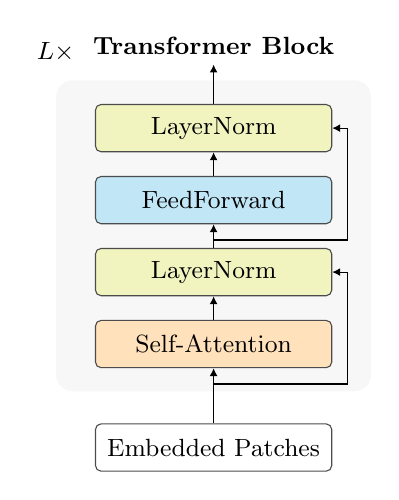
\begin{tikzpicture}[
      font=\small,
      >={Latex[length=1mm,width=1mm]},
      layer/.style={rounded corners=2pt, draw=black!70, minimum width=3cm, minimum height=6mm, align=center},
      layernorm/.style={layer, fill=ln},
      selfattn/.style={layer, fill=sa},
      feedforward/.style={layer, fill=ff},
]

\node[rounded corners=6pt, minimum width=40mm, minimum height=39.5mm, fill=black!3, anchor=north west] (transformer_block) {};
\node[above=2mm of transformer_block.north] (title) {\textbf{Transformer Block}};

\node[layer, below=4mm of transformer_block.south, anchor=north] (emb) {Embedded Patches};
\node[selfattn, above=3mm of transformer_block.south] (sa) {Self-Attention};
\node[layernorm, above=3mm of sa] (ln1) {LayerNorm};
\coordinate (sa_south_east) at ($(sa.south)+(17mm,-2mm)$);

\draw[->] (emb.north) -- (sa.south);
\draw[->] (sa.north) -- (ln1.south);
\draw[->] ($(sa.south)+(0mm,-2mm)$) -- (sa_south_east) |- ($(ln1.east)+(0mm,0mm)$);

\node[feedforward, above=3mm of ln1] (ff) {FeedForward};
\node[layernorm, above=3mm of ff] (ln2) {LayerNorm};
\coordinate (ff_south_east) at ($(ff.south)+(17mm,-2mm)$);

\draw[->] (ln1.north) -- (ff.south);
\draw[->] (ff.north) -- (ln2.south);
\draw[->] (ln2.north) -- ($(ln2.north)+(0mm,5mm)$);
\draw[->] ($(ff.south)+(0mm,-2mm)$) -- (ff_south_east) |- ($(ln2.east)+(0mm,0mm)$);

\node[above=1mm of transformer_block.north west] {$L\times$};

\end{tikzpicture}
\caption{Transformer architecture we use in our experiments}
\label{fig:transformer}
\vspace{-2em}
\end{wrapfigure}

To verify our theoretical estimates we conduct a comprehensive empirical study. We follow the same Transformer architecture we used in the main part of the paper, which is essentially post-norm (LayerNorm is after Self-Attention/FeedForward).

In particular, we consider an image classification task, implementing the Vision Transformer (ViT) architecture similar to~\cite{dosovitskiy2020image}, see Figure~\ref{fig:transformer}. Input image is patchified with linear projection and then goes to Transformer Encoder, which contains $L$ Transformer Blocks, while its outputs is averaged to obtain classification logits.

\textbf{Hessian entries visualization. } In this part we use a single Transformer block, which we train on a MNIST~\cite{deng2012mnist} dataset (see~\ref{table:vit}). Firstly, we put just one batch from a train dataloader to the initialized model and calculate the exact Hessian using \href{https://curvlinops.readthedocs.io/en/latest/#}{\texttt{curvlinops}} Python package for an efficient Hessian linear operator calculation. Visualizing it in a log-scale, in Figure~\ref{fig:hessian_entries} we emphasize the heterogenity in the magnitues of the entries.

\begin{table}[H]
    \centering
    \begin{tabular}{c|cccc}
        dataset & patch size & hidden dim & ff dim & num blocks  \\
        \hline
        MNIST & 4 & 16 & 64 & 1 \\
        CIFAR-100 & 4 & 128 & 512 & 8 \\
    \end{tabular}
    \caption{Vision Transformer (ViT) architectures hyperparameters we use in our experiments}
    \label{table:vit}
\end{table}

\begin{figure}[H]
    \centering
    \includegraphics[width=0.72\linewidth]{figs/hessian_entries.pdf}
    \caption{Hessian entries visualization for \textbf{an initialized model} with one Transformer Block. We see the entire magnitudes' heterogeneity, while the \textcolor{olive}{Values} corresponding blocks have larger values.}
    \label{fig:hessian_entries}
\end{figure}
We train the model for a number of epochs, obtaining pretty high accuracy on a validation dataset (>50\%), and then visualize the Hessian's entries again, see Figure~\ref{fig:hessian_entries_trained}. One can see that each of the Hessian's blocks becomes more magnituted, however the \textcolor{olive}{Values}-\textcolor{olive}{Values} block exhibits the highest one.

\begin{figure}[H]
    \centering
    \includegraphics[width=0.72\linewidth]{figs/hessian_entries_trained.pdf}
    \caption{Hessian entries visualization for \textbf{a model trained for a number of epochs} with one Transformer Block. We see the entire magnitudes' heterogeneity, while the \textcolor{olive}{Values}-\textcolor{olive}{Values} corresponding block has the largest values.}
    \label{fig:hessian_entries_trained}
\end{figure}
\noindent
This experiment shows exactly how the entire Transformer's Hessian is organized, which allows us to investigate each block part of it separately. In Appendix \ref{app:exp_changing_over_epochs} we continue this experiment by providing Parameters blocks changing over training epochs figures.

Further, we calculate the matrices' norms and their Hessians' norms, and show them in Figure~\ref{fig:norm}

\begin{figure}[H]
    \centering
    \includegraphics[width=0.43\linewidth]{figs/parameters_norm.pdf}\hfill
    \includegraphics[width=0.43\linewidth]{figs/hessians_norm.pdf}
    \caption{Parameters' blocks norms and their Hessians' norms, calculated exactly on one batch containing 128 examples from the MNIST training dataset.}
    \label{fig:norm}
\end{figure}

Results show that the highest magnitude corresponds to the Keys and Values, while the other blocks exhibit much smaller absolute entries.

\textbf{Loss landscape convergence. } To further deep inside the dependence between loss function and its Hessian, we conduct and experiment corresponding to Theorem~\ref{thm:convergence}. Here we employ the other model configuration on a CIFAR-100~\cite{krizhevsky2009learning} dataset. Compared to similar one for a MNIST dataset, this model have $8\times$ more Transformer blocks and also $8\times$ wider hidden layers. During traning, it is also trained for a number of epochs to achieve >50\% Accuracy on a validation dataset. The results are in Figure \ref{fig:loss_landscape_convergence}.  The experiment setup is as follows:
\begin{enumerate}
    \item Train the model until convergence and save the parameters $\mathbf{w*}$ (model checkpoint);
    \item Start from the empty dataset, add data batch-by-batch and calculate mean loss value over the seen batches;
    \item Calculate the absolute difference according to $\left| \mathcal{L}_{k+1}(\mathbf{w}) - \mathcal{L}_k(\mathbf{w}) \right|$.
\end{enumerate}

Our code is available at \url{https://github.com/modernTalker/transformer_hessian.git}
\newpage

\begin{wrapfigure}{r}{0.5\textwidth}
\centering
\vspace{-2.5em}
\includegraphics[width=0.5\textwidth]{figs/loss_landscape_convergence.pdf}
\caption{Absolute loss difference vs. the number of training samples in the dataset, plotted in log-log scale. The \textcolor{blue}{blue} line represents the EMA of a desired dependency, while the \textcolor{gray}{gray} one corresponds to the linear trend.}
\label{fig:loss_landscape_convergence}
\vspace{-2em}
\end{wrapfigure}

\section{Discussion and Conclusion}\label{sec:disc}

This work fills a key gap in the second-order analysis of Transformers by deriving explicit Jacobians and Hessians for LayerNorm and FFN in the $\mathrm{vec}_r$ numerator-layout, and integrating them into a full block-level curvature decomposition. Theorems~\ref{thm:layernorm_derivative}-\ref{thm:layernorm_second_derivative} and \ref{thm:transformer_derivative}-\ref{thm:transformer_hessian} yield end-to-end expressions that are compatible with Kronecker structure and commutation identities, while Theorems~\ref{thm:self_attention_hessian_estimation} and \ref{thm:transformer_hessian_estimate} provide spectral-norm bounds that connect curvature to input statistics, LayerNorm scales, and architectural hyperparameters. A direct consequence is a block-heterogeneous Hessian: Value- and Key-related terms dominate through softmax derivatives and input-dependent operators, FFN curvature is controlled by the piecewise linearity of ReLU, and LayerNorm contributes via per-row variance. The empirical results (e.g., Figures~\ref{fig:hessian_entries} and \ref{fig:hessian_entries_trained}) match these predictions, with Values - Values blocks exhibiting the largest magnitudes after training.

The second-order Taylor expansion in Theorem~\ref{thm:convergence} gives a compact convergence inequality, $|\mathcal{L}_{k+1}(\mathbf{w})-\mathcal{L}_{k}(\mathbf{w})| \le 2L/(k+1) + M\|\mathbf{w}-\mathbf{w}^*\|_2^2/(k+1)$, where $M$ as a function of input data is provided by our Hessian bounds \ref{thm:self_attention_hessian_estimation}, \ref{thm:transformer_hessian_estimate}. This explains the observed stabilization of the loss landscape with increasing data. The log–log trend in Figure~\ref{fig:loss_landscape_convergence} follows this prediction, supporting the claim that increasing data size stabilizes the local geometry of the Transformer objective. Finally, the block-wise structure motivates curvature-aware training through per-block adaptation of learning rates, weight decay, or preconditioning, and provides a mechanistic rationale for switching from data scaling to model scaling near curvature stationarity, consistent with compute-optimal policies \cite{kaplan2020scaling,hoffmann2022training}.

The analysis is local and assumes a shared minimizer for consecutive dataset sizes (Assumption~\ref{as:zero_grad}). The present theoretical derivation focuses on a single-head, post-normalization transformer block under the mean-squared error loss. While extensions to multi-head attention, masking, and positional encodings are technically feasible within the established calculus, they are omitted for brevity. It should be emphasized that the underlying framework naturally generalizes to the cross-entropy loss, a generalization that has been explicitly validated in our experimental section \ref{sec:exp}. A primary direction for future work involves extending this analysis to deep, multi-layer transformer architectures.

% The theoretical and empirical findings presented in this paper provide significant insights into the convergence behavior of the loss function surface in transformer neural network architectures as the dataset size increases. Our analysis, grounded in the Hessian-based approach, extends prior work by explicitly addressing the impact of dataset size on the loss landscape, a relatively underexplored area for transformers. The derived bounds, as stated in Theorems~\ref{thm:self_attention_hessian_estimation} and~\ref{thm:self_attantion_convergence}, offer a rigorous framework for understanding how the loss function stabilizes and the minimum dataset size required to achieve a predetermined error threshold.

% The empirical results, particularly from the transformer-specific experiments with the Vision Transformer (ViT), confirm that the difference \( |\mathcal{L}_{k+1}(\mathbf{w}) - \mathcal{L}_k(\mathbf{w})| \) decreases as the dataset size \( k \) grows, aligning with our theoretical predictions. This convergence is visually demonstrated in Figure~\ref{fig:mnist_ranks}, where the loss function difference diminishes monotonically, suggesting that beyond a certain dataset size, additional data contribute marginally to altering the loss landscape. This observation has practical implications, especially in domains where data collection is resource-intensive, such as medical imaging or specialized image classification tasks. By identifying a sufficient dataset size \( k^* \), practitioners can optimize computational resources and reduce training costs without sacrificing model performance.

% Our findings also highlight the importance of the Hessian spectrum in understanding the geometry of the loss landscape. The boundedness of the Hessian norm, as derived in Theorem~\ref{thm:self_attention_hessian_estimation}, indicates that the curvature of the loss surface is constrained by architectural parameters (e.g., \( W_{\text{max}}, X_{\text{max}} \)) and dataset characteristics. This insight can guide the design of transformer architectures by balancing model complexity with dataset size to achieve efficient training. Moreover, the empirical validation using techniques like LoRA and unfreezing the last layers demonstrates the robustness of our theoretical results across different fine-tuning strategies, suggesting applicability to real-world scenarios where pre-trained models are adapted to specific tasks.

% However, our study has limitations. The theoretical analysis assumes a local minimum at \( \mathbf{w}^* \) and relies on the second-order Taylor approximation, which may not fully capture the global behavior of the loss landscape. Additionally, the experiments focus primarily on vision tasks with ViT, and further studies are needed to generalize these findings to other transformer-based models, such as those used in natural language processing. Future work could explore the impact of different loss functions, regularization techniques, or dataset distributions on convergence behavior. Extending the analysis to multi-layer transformers or other attention mechanisms could also provide deeper insights into the scalability of our results.

% In summary, our work bridges a critical gap in understanding the relationship between dataset size and loss landscape convergence in transformers. The proposed framework not only advances theoretical understanding but also offers practical guidance for efficient model training, particularly in data-constrained settings.

% \section{Conclusion}\label{sec:concl}

% In this paper, we investigated the convergence of the loss function surface in transformer neural network architectures with respect to increasing dataset size. By leveraging a Hessian-based analysis, we derived theoretical bounds on the difference between loss functions for consecutive dataset sizes, as formalized in Theorems~\ref{thm:self_attention_hessian_estimation} and~\ref{thm:self_attantion_convergence}. These bounds provide a precise estimate of the minimum dataset size required to achieve a specified error tolerance, offering a novel perspective on the interplay between data volume and model training efficiency.

% Our empirical studies, conducted on real-world vision tasks using the Vision Transformer, validate the theoretical predictions. The observed monotonic decrease in \( |\mathcal{L}_{k+1}(\mathbf{w}) - \mathcal{L}_k(\mathbf{w})| \) confirms that the loss landscape stabilizes as more data are included, with practical implications for optimizing data collection and computational resources. These results are particularly relevant for applications where acquiring large datasets is challenging, enabling practitioners to make informed decisions about dataset size requirements.

% The proposed approach advances the understanding of transformer loss landscapes and sets the stage for future research. Potential directions include extending the analysis to other transformer variants, exploring global loss landscape properties, and investigating the role of dataset diversity in convergence behavior. By providing a robust theoretical and empirical foundation, this work contributes to the efficient design and training of transformer-based models, paving the way for more resource-efficient deep learning practices.


%%%%%%%%%%%%%%%%%%%%%%%%%%%%%%%%%%%%%%%%%%%%%%%%%%%%%%%%%%%%

\bibliographystyle{unsrtnat}
\bibliography{references}

%%%%%%%%%%%%%%%%%%%%%%%%%%%%%%%%%%%%%%%%%%%%%%%%%%%%%%%%%%%%

\newpage
\appendix
\section{Appendix / supplemental material}\label{app:A}

\subsection{Parameters blocks changing over training epochs.}\label{app:exp_changing_over_epochs}

Here we continue the previous experiments, expanding the plots into separate parameters blocks entries changing. Again, we employ the MNIST's dataset version of our model (Figure~\ref{table:vit}). We log the matrices entries, norms, and Hessians during the first 1000 training steps. As we can see on Figures~\ref{fig:hessian_entries_queries},~\ref{fig:hessian_entries_keys},~\ref{fig:hessian_entries_values},~\ref{fig:hessian_entries_layernorm},~\ref{fig:hessian_entries_feedforward}.

\begin{figure}[H]
    \centering
    \includegraphics[width=\linewidth]{figs/hessian_entries_queries.pdf}
    \caption{Queries entries visualization.}
    \label{fig:hessian_entries_queries}
\end{figure}

\begin{figure}[H]
    \centering
    \includegraphics[width=\linewidth]{figs/hessian_entries_keys.pdf}
    \caption{Keys entries visualization.}
    \label{fig:hessian_entries_keys}
\end{figure}

\begin{figure}[H]
    \centering
    \includegraphics[width=\linewidth]{figs/hessian_entries_values.pdf}
    \caption{Values entries visualization.}
    \label{fig:hessian_entries_values}
\end{figure}

\begin{figure}[H]
    \centering
    \includegraphics[width=\linewidth]{figs/hessian_entries_layernorm.pdf}
    \caption{LayerNorm entries visualization.}
    \label{fig:hessian_entries_layernorm}
\end{figure}

\begin{figure}[H]
    \centering
    \includegraphics[width=\linewidth]{figs/hessian_entries_feedforward.pdf}
    \caption{FeedForward entries visualization.}
    \label{fig:hessian_entries_feedforward}
\end{figure}

\subsection{Assumptions validation}\label{app:exp_assumption_check}

In this section we provide experimental validation of the assumptions stated in the text. Since Assumption \ref{as:non_zero_variance} is technical, we focus on empirically validating Assumption \ref{as:zero_grad}.

\begin{figure}[H]
    \centering
    \includegraphics[width=0.8\linewidth]{figs/assumption_1.pdf}
    \caption{Validation of Assumption \ref{as:zero_grad}}
    \label{fig:ass_1_validation}
\end{figure}

Figure \ref{fig:ass_1_validation} presents the corresponding results, indicating that while Assumption \ref{as:zero_grad} can be relaxed, its validity increases with longer sequence lengths (i.e., a larger number of samples).

\section{Appendix / Matrix calculus preliminaries} \label{app:properties}

\subsection{Basic matrix operations properties}

First, we define the notations and rules that we actively use in the text.

\begin{definition}[Matrix Norms] \label{def:matrix_norms}
For a matrix $\mathbf{A} \in \mathbb{R}^{m \times n}$:
\begin{align*}
\|\mathbf{A}\|_2 &= \sigma_1 \quad &&\text{(Spectral norm, largest singular value)} \\
\|\mathbf{A}\|_F &= \sqrt{\sum_{i=1}^m \sum_{j=1}^n |a_{ij}|^2} = \sqrt{\sum_{i=1}^r \sigma_i^2} \quad &&\text{(Frobenius norm)} \\
\|\mathbf{A}\|_1 &= \max_{1 \leq j \leq n} \sum_{i=1}^m |a_{ij}| \quad &&\text{(Maximum absolute column sum)} \\
\|\mathbf{A}\|_\infty &= \max_{1 \leq i \leq m} \sum_{j=1}^n |a_{ij}| \quad &&\text{(Maximum absolute row sum)} \\
\|\mathbf{A}\|_{\max} &= \max_{i,j} |a_{ij}| \quad &&\text{(Element-wise maximum, not a submultiplicative norm)}
\end{align*}
\end{definition}

\begin{definition}[Vectorization and Element-wise Operations] \label{def:vec_elem_ops}
Let $\mathbf{A}$ be a matrix and $\mathbf{v}$ be a vector.
\begin{itemize}
    \item $\mathrm{vec}_r(\mathbf{A})$ denotes the row-wise vectorization of matrix $\mathbf{A}$.
    \item $\mathbf{A}^{\circ \alpha}$ denotes the element-wise $\alpha$-power of matrix $\mathbf{A}$, i.e., $(\mathbf{A}^{\circ \alpha})_{ij} = (\mathbf{A}_{ij})^\alpha$.
    \item $\textit{diag}(\mathbf{v})$ creates a diagonal matrix with vector $\mathbf{v}$ on its main diagonal.
\end{itemize}
\end{definition}

\begin{property}[Relation between $\mathrm{vec}$ and $\mathrm{vec}_r$] \label{prop:vec_relation}
    Let $\mathbf{A} \in \mathbb{R}^{m \times n}$. The row-wise vectorization operator $\mathrm{vec}_r$ and the standard column-wise vectorization operator $\mathrm{vec}$ are related by the transpose:
\begin{equation*}
\mathrm{vec}_r(\mathbf{A}) = \mathrm{vec}(\mathbf{A}^\top)
\end{equation*}
\end{property}

\begin{definition}[Commutation Matrix] \label{def:commutation_matrix}

The commutation matrix $\mathbf{K}_{m,n} \in \mathbb{R}^{mn \times mn}$ is the unique matrix such that for any matrix $\mathbf{A} \in \mathbb{R}^{m \times n}$ the following holds

\begin{equation*}
\mathbf{K}_{m,n} \mathrm{vec}(\mathbf{A}) = \mathrm{vec}(\mathbf{A}^\top)
\end{equation*}

Using Property \ref{prop:vec_relation}, we immediately have the relationship:

\begin{equation*}
\mathrm{vec}_r(\mathbf{A}) = \mathbf{K}_{m,n} \mathrm{vec}(\mathbf{A}) \quad \text{and} \quad \mathrm{vec}(\mathbf{A}) = \mathbf{K}_{n,m} \mathrm{vec}_r(\mathbf{A})
\end{equation*}

since $\mathbf{K}_{n,m}\mathbf{K}_{m,n} = \mathbf{I}_{mn}$.
\end{definition}

From \cite{magnus1988matrix} we utilize the property

\begin{property} [Row-wise vectorization of matrix product] \label{prop:vec_r_matrix_product}
    Let $\mathbf{X}, \mathbf{A}, \mathbf{B}$ be matrices with appropriate dimensions, then
    \begin{equation*}
        \mathrm{vec}_r(\mathbf{A} \mathbf{X}\mathbf{B}) = (\mathbf{A} \otimes \mathbf{B}^\top) \mathrm{vec}_r(\mathbf{X})
    \end{equation*}
\end{property}

\begin{property}[Row-wise vectorization of Hadamard product] \label{prop:vec_r_hadamard_product}
Let $\mathbf{A}, \mathbf{B} \in \mathbb{R}^{m \times n}$. Then

\[
\mathrm{vec}_r(\mathbf{A} \circ \mathbf{B}) = \textit{diag}(\mathrm{vec}_r(\mathbf{A})) \mathrm{vec}_r(\mathbf{B})
\]

where $\circ$ denotes the Hadamard (element-wise) product.
This result follows directly from \cite{magnus1988matrix}, where the similar result was obtained for column-wise vectorization. 
\end{property}

\begin{proposition} [Identification Theorem for Row-wise Vectorization] \label{prop:identification_theorem_vec_r}

Let $\mathbf{F}: \mathbb{R}^{m\times n} \rightarrow \mathbb{R}^{p, q}$ be a differentiable matrix-valued function of a matrix $\mathbf{X} \in \mathbb{R}^{m \times n}$. If the differential of $\mathbf{F}$ can be written as \begin{equation*}
d \mathrm{vec}_r(\mathbf{F}(\mathbf{X})) = \mathbf{J} \cdot d \mathrm{vec}_r(\mathbf{X})
\end{equation*}

for some matrix $\mathbf{J} \in \mathbb{R}^{pq \times mn}$ that does not depend on $d\mathbf{X}$. Then $\mathbf{J}$ is the Jacobian matrix of the transformation from $\mathbf{X}$ to $\mathbf{F}(\mathbf{X})$ with respect to row-wise vectorization. We denote this as:

\begin{equation*}
\frac{\partial \mathbf{F}(\mathbf{X})}{\partial \mathbf{X}} := \frac{\partial \mathrm{vec}_r(\mathbf{F}(\mathbf{X}))}{\partial (\mathrm{vec}_r(\mathbf{X}))^\top} = \mathbf{J}
\end{equation*}

This is the $\mathrm{vec}_r$ analogue of the fundamental Identification Theorem from \cite{magnus1988matrix} for column-wise vectorization.
    
\end{proposition}

\begin{property}[Element-wise division] \label{prop:elem_wise_division}
    Let $\mathbf{A} \in \mathbb{R}^{m\times n}$ be a matrix and $\mathbf{b} \in \mathbb{R}^{m \times 1}$ be a vector. Then for matrix $\mathbf{C} \in {\in \mathbb{R}^{m \times n}}$, where $c_{i,j} = \frac{a_{i,j}}{b_i}$ is fulfilled that
    \begin{equation*}
        \mathbf{C} = \textit{diag}^{-1}(\mathbf{b})\mathbf{A}
    \end{equation*}
\end{property}

\begin{proposition} [Spectral norm of $\mathbf{1}_{L \times L}$ matrix] \label{prop:1_spectral_norm}
    Let $\mathbf{A} = \mathbf{1}_{L \times L}$ (a matrix full of 1). Then its spectral norm is
    \begin{equation*}
        \| \mathbf{A}\|_2 = L
    \end{equation*}
\end{proposition}

\begin{proof}
    Using basic Linear Algebra properties, we obtain $\mathrm{tr}(\mathbf{A}) = L$ and $\mathrm{rank}(\mathbf{A}) = 1 = \mathrm{dim}(\mathrm{Im}(\mathbf{X}))$. Therefore, using $\mathrm{dim}(\mathrm{Im}(\mathbf{X})) + \mathrm{dim}(\mathrm{Ker}(\mathbf{X})) = L$, we get $\mathrm{dim}(\mathrm{Ker}(\mathbf{X})) = L - 1$. Thus, for $i \in \{2, \dots L\}$ we get $\lambda_i = 0$ and for $\lambda_1 = L$. Then, the only non-null singular value of the matrix $\mathbf{A}$ is $\sqrt{L^2} = L$. Thus, we obtain that $\| \mathbf{A}\|_2 = L$, according to Definition \ref{def:matrix_norms}.
\end{proof}
    
\subsection{Matrix-valued functions derivative properties}

Next, we introduce the properties for calculating the matrix-valued function derivative.

\begin{property} [Matrix-Product derivative] \label{prop:matrix_product_derivative}
    Let $\mathbf{X}, \mathbf{A}, \mathbf{B}$ be matrices with appropriate dimensions, then
    \begin{equation*}
        \frac{\partial\mathbf{A}\mathbf{X}\mathbf{B}}{\partial\mathbf{X}} = \mathbf{A} \otimes \mathbf{B}^\top
    \end{equation*}
    where $\mathbf{A}$ and $\mathbf{B}$ have no dependence on $\mathbf{X}$.
\end{property}

Detailed proof of this statement can be found in \cite{singh2021analyticinsightsstructurerank}.

\begin{property} [Kronecker-Product derivative] \label{prop:kronecker_product_derivative}
    Let \( \mathbf{X} \in \mathbb{R}^{n \times q} \) and \( \mathbf{Y} \in \mathbb{R}^{p \times r} \). Then
\[
\frac{\partial (\mathbf{X} \otimes \mathbf{Y})}{\partial \mathbf{X}} = (\mathbf{I}_n \otimes \mathbf{K}_{p,q} \otimes \mathbf{I}_r) \left( \mathbf{I}_{nq} \otimes \mathrm{vec}_r \mathbf{Y} \right),
\]
and analogously
\[
\frac{\partial (\mathbf{X} \otimes \mathbf{Y})}{\partial \mathbf{Y}} = (\mathbf{I}_n \otimes \mathbf{K}_{p,q} \otimes \mathbf{I}_r) \left( \mathrm{vec}_r \mathbf{X} \otimes \mathbf{I}_{pr} \right).
\]
\end{property}

The detailed proof is in \cite{ormaniec2024attentionhessian}.

From the properties above, we derive calculations for special cases which we use in this paper.

\begin{proposition} [Matrix-valued functions multiplication derivative] \label{prop:matrix_funcs_product_derivative}

Let  $\mathbf{A}(\mathbf{X}) \in \mathbb{R}^{p \times r}$ and $\mathbf{B}(\mathbf{X}) \in \mathbb{R}^{r \times q}$ be matrix-valued functions of the matrix $\mathbf{X}$, then

\begin{equation*}
    \frac{\partial\mathbf{A}(\mathbf{X}) \mathbf{B}(\mathbf{X})}{\partial \mathbf{X}} = \left(\mathbf{A} \otimes \mathbf{I}_q 
 \right) \frac{\partial\mathbf{B}}{\partial\mathbf{X}} + \left( \mathbf{I}_p \otimes \mathbf{B}^\top\right) \frac{\partial\mathbf{A}}{\partial\mathbf{X}}
\end{equation*}
    
\end{proposition}

\begin{proof}
    First, we apply  a classic chain-rule for calculation a derivative of a complicated function and then combine it with Property \ref{prop:matrix_product_derivative}
    \begin{align*}
        \frac{\partial\mathbf{A}(\mathbf{X}) \mathbf{B}(\mathbf{X})}{\partial \mathbf{X}} &= \frac{\partial \mathbf{A}\mathbf{B}}{\partial\mathbf{B}}\frac{\partial\mathbf{B}}{\partial \mathbf{X}} + \frac{\partial \mathbf{A}\mathbf{B}}{\partial\mathbf{A}}\frac{\partial\mathbf{A}}{\partial \mathbf{X}} = \frac{\partial \mathbf{A}\mathbf{B}\mathbf{I}_q}{\partial\mathbf{B}}\frac{\partial\mathbf{B}}{\partial \mathbf{X}} + \frac{\partial \mathbf{I}_p\mathbf{A}\mathbf{B}}{\partial\mathbf{A}}\frac{\partial\mathbf{A}}{\partial \mathbf{X}} = \\
        &= \left( \mathbf{A} \otimes \mathbf{I}_q \right) \frac{\partial \mathbf{B}}{\partial \mathbf{X}} + \left( \mathbf{I}_p \otimes \mathbf{B}^\top \right) \frac{\partial \mathbf{A}}{\partial \mathbf{X}}
    \end{align*}
\end{proof}

\begin{proposition} [Matrix-valued functions Kronecker product derivative] \label{prop:matrix_funcs_kronecker_product_derivative}

Let  $\mathbf{A}(\mathbf{X}) \in \mathbb{R}^{n \times q}$ and $\mathbf{B}(\mathbf{X}) \in \mathbb{R}^{p \times r}$ be matrix-valued functions of the matrix $\mathbf{X}$, then

\begin{equation*}
    \frac{\partial\mathbf{A}(\mathbf{X}) \otimes \mathbf{B}(\mathbf{X})}{\partial \mathbf{X}} = (\mathbf{I}_n \otimes \mathbf{K}_{p,q} \otimes \mathbf{I}_r) \left( \left( \mathrm{vec}_r \mathbf{A} \otimes \mathbf{I}_{pr} \right) \frac{\partial\mathbf{B}}{\partial \mathbf{X}} + \left( \mathbf{I}_{nq} \otimes \mathrm{vec}_r \mathbf{B} \right) \frac{\partial\mathbf{A}}{\partial \mathbf{X}}\right)
\end{equation*}
    
\end{proposition}

\begin{proof}
    First, we apply a classic chain rule for calculating the derivative of a complicated function and then combine it with Property \ref{prop:kronecker_product_derivative}
    \begin{align*}
        \frac{\partial\mathbf{A}(\mathbf{X}) \otimes \mathbf{B}(\mathbf{X})}{\partial \mathbf{X}} &= \frac{\partial \mathbf{A}\otimes\mathbf{B}}{\partial\mathbf{B}}\frac{\partial\mathbf{B}}{\partial \mathbf{X}} + \frac{\partial \mathbf{A}\otimes\mathbf{B}}{\partial\mathbf{A}}\frac{\partial\mathbf{A}}{\partial \mathbf{X}} = \\
        &= (\mathbf{I}_n \otimes \mathbf{K}_{p,q} \otimes \mathbf{I}_r) \left( \mathrm{vec}_r \mathbf{A} \otimes \mathbf{I}_{pr} \right) \frac{\partial\mathbf{B}}{\partial \mathbf{X}} + (\mathbf{I}_n \otimes \mathbf{K}_{p,q} \otimes \mathbf{I}_r) \left( \mathbf{I}_{nq} \otimes \mathrm{vec}_r \mathbf{B} \right) \frac{\partial\mathbf{A}}{\partial \mathbf{X}} = \\
        &= (\mathbf{I}_n \otimes \mathbf{K}_{p,q} \otimes \mathbf{I}_r) \left( \left( \mathrm{vec}_r \mathbf{A} \otimes \mathbf{I}_{pr} \right) \frac{\partial\mathbf{B}}{\partial \mathbf{X}} + \left( \mathbf{I}_{nq} \otimes \mathrm{vec}_r \mathbf{B} \right) \frac{\partial\mathbf{A}}{\partial \mathbf{X}}\right)
    \end{align*}
\end{proof}

Next, we develop the operations that we introduced above and derive calculations using $\mathrm{\text{vec}}_r$ notation as we do in this paper.

\begin{proposition} [Derivative of the invert matrix] \label{prop:invert_derivative}
For an invertible square matrix $\mathbf{D} \in \mathbb{R}^{n \times n}$, the derivative of its inverse is
\[
    \frac{\partial \mathbf{D}^{-1}}{\partial \mathbf{D}} 
    = -\mathbf{D}^{-1} \otimes \mathbf{D}^{-\top}.
\]
\end{proposition}

\begin{proof}
This is a standard result in matrix calculus. The differential identity 
\[
    d(\mathbf{D}^{-1}) = -\mathbf{D}^{-1} \,(d\mathbf{D})\, \mathbf{D}^{-1}
\]
appears in \cite{petersen2012matrix} and in \cite{magnus1988matrix}.  
Applying the $\mathrm{vec}_r$ operator and using the property \ref{prop:vec_r_matrix_product} yields 

\[
\mathrm{vec}_r(-\mathbf{D}^{-1} \,(d\mathbf{D})\, \mathbf{D}^{-1}) = (-\mathbf{D}^{-1} \otimes \mathbf{D}^{-\top}) \mathrm{vec}_r(d\mathbf{D})
\]

By the definition and the identification theorem from Property \ref{prop:identification_theorem_vec_r} we obtain

\[
\mathrm{vec}_r(d\mathbf{D}^{-1}) = \frac{\partial \mathrm{vec}_r \mathbf{D}^{-1}}{\partial\mathrm{vec}_r\mathbf{D}} \mathrm{vec}_r(d\mathbf{D})
\]

Comparing two results we get $\frac{\partial \mathrm{vec}_r \mathbf{D}^{-1}}{\partial\mathrm{vec}_r\mathbf{D}} = (-\mathbf{D}^{-1} \otimes \mathbf{D}^{-\top})$

\end{proof}

\begin{proposition}[Derivative of $\mathrm{diag}(\cdot)$] \label{prop:diag_derivative}
For $\mathbf{v} \in \mathbb{R}^{L \times 1}$, the derivative of the diagonalization map is
\[
    \frac{\partial \mathrm{diag}(\mathbf{v})}{\partial \mathbf{v}}
    = \big(\mathbf{e}_1 \otimes \mathbf{e}_1 \quad \dots \quad \mathbf{e}_L \otimes \mathbf{e}_L\big),
\]
where $\mathbf{e}_i$ are the standard basis vectors in $\mathbb{R}^L$.
\end{proposition}

\begin{proof}
By Definition \ref{def:vec_elem_ops}, $\mathrm{diag}(\mathbf{v})$ places entry $v_i$ at position $(i,i)$ of the resulting diagonal matrix.

The derivative of $\mathrm{diag}(\mathbf{v})$ w.r.t.\ $v_i$ is the elementary matrix $\mathbf{E}_{ii} = \mathbf{e}_i \mathbf{e}_i^\top$ that has one in position $(i,i)$ and zeros elsewhere.

Applying the row-wise vectorization operator, we obtain
\[
\mathrm{vec}_r(\mathbf{E}_{i,i}) = \mathbf{e}_i \otimes \mathbf{e}_i
\]

by the standard Kronecker–vec identity \ref{prop:vec_r_matrix_product}.

Stacking across $i=1,\dots,L$, the Jacobian becomes

\[
    \frac{\partial \mathrm{diag}(\mathbf{v})}{\partial \mathbf{v}}
    = \big(\mathbf{e}_1 \otimes \mathbf{e}_1 \quad \dots \quad \mathbf{e}_L \otimes \mathbf{e}_L\big),
\]
\end{proof}


\begin{proposition}[Derivative of the Hadamard square] \label{prop:hadamard_square_derivative}
For a matrix $\mathbf{A} \in \mathbb{R}^{m \times n}$, the derivative of the elementwise square is
\[
    \frac{\partial \mathbf{A}^{\circ 2}}{\partial \mathbf{A}}
    = 2 \cdot \mathrm{diag}\!\big(\mathrm{vec}_r(\mathbf{A})\big).
\]
\end{proposition}

\begin{proof}
By Definition \ref{def:vec_elem_ops}, $(\mathbf{A}^{\circ 2}){ij} = (\mathbf{A}{ij})^2$.
Differentiating elementwise gives $d(\mathbf{A}^{\circ 2}) = 2\mathbf{A} \circ d\mathbf{A}$.
Applying the $\mathrm{vec}_r$ operator and using Property~\ref{prop:vec_r_hadamard_product}, we obtain
\[
    \mathrm{vec}_r(d(\mathbf{A}^{\circ 2})) = 2 \textit{diag}(\mathrm{vec}_r(\mathbf{A})) \mathrm{vec}_r (d\mathbf{A})
\]

By the identification theorem from Property \ref{prop:identification_theorem_vec_r}, this implies

\[
    \frac{\partial \mathbf{A}^{\circ 2}}{\partial \mathbf{A}}
    = \frac{\partial \mathrm{vec}_r(\mathbf{A}^{\circ 2})}{\partial \mathrm{vec}_r(\mathbf{A})} = 2 \cdot \mathrm{diag}\!\big(\mathrm{vec}_r(\mathbf{A})\big)
\]

which establishes the result.
\end{proof}


\begin{proposition}[Derivative of the Hadamard root]\label{prop:hadamard_root_derivative}
For $\mathbf{A} \in \mathbb{R}^{m \times n}$ with positive entries, the derivative of the elementwise square root is
\[
    \frac{\partial \mathbf{A}^{\circ \frac{1}{2}}}{\partial \mathbf{A}}
    = \tfrac{1}{2}\, \mathrm{diag}^{-1}\!\big(\mathrm{vec}_r^{\circ \frac{1}{2}}(\mathbf{A})\big).
\]
\end{proposition}
\begin{proof}
Similarly to the proof of Proposition \ref{prop:hadamard_square_derivative}, we obtain $d(\mathbf{A}^{\circ 1/2}) = \frac{1}{2}\mathbf{A}^{\circ -1/2} \circ d\mathbf{A}$ 
Thus, writing in vectorized form gives
\[
    \frac{\partial \mathbf{A}^{\circ \frac{1}{2}}}{\partial \mathbf{A}}
    = \frac{\partial \mathrm{vec}_r(\mathbf{A}^{\circ \frac{1}{2}})}{\partial \mathrm{vec}_r(\mathbf{A})} = \tfrac{1}{2}\, \mathrm{diag}^{-1}\!\big(\mathrm{vec}_r^{\circ \frac{1}{2}}(\mathbf{A})\big).
\]
\end{proof}

\begin{proposition} [Transposed Matrix derivative] \label{prop:transposed_matrix_derivative}

Let $\mathbf{A} \in \mathbb{R}^{m \times n}$, then the following holds:

\begin{equation*}
    \frac{\partial \mathbf{A}^\top}{\partial \mathbf{A}} = \mathbf{K}_{n, m}
\end{equation*}
    
\end{proposition} 

\begin{proof}
    Combining a similar property from \cite{magnus1988matrix} for column-wise vectorization with the column-row connection rule \ref{prop:vec_relation} and \ref{def:commutation_matrix} we obtain the theorem statement.
\end{proof}


\subsection{Matrix norm properties}

Similarly to \cite{petersen2012matrix} we introduce a matrix norms table comparison.

\begin{property}[Matrix norm inequalities] \label{prop:matrix_norm_inequalities}
Let $\mathbf{A} \in \mathbb{R}^{m \times n}$. Then the following inequalities hold between different matrix norms:

\begin{center}
\renewcommand{\arraystretch}{1.5}
\begin{tabular}{c|ccccc}
\diagbox[height=2em, width=4em]{X}{Y} & $\|\mathbf{A}\|_{\max}$ & $\|\mathbf{A}\|_1$ & $\|\mathbf{A}\|_\infty$ & $\|\mathbf{A}\|_2$ & $\|\mathbf{A}\|_F$ \\
\hline
$\|\mathbf{A}\|_{\max}$ &  & 1 & 1 & 1 & 1 \\
$\|\mathbf{A}\|_1$ & $m$ &  & $m$ & $\sqrt{m}$ & $\sqrt{m}$ \\
$\|\mathbf{A}\|_\infty$ & $n$ & $n$ &  & $\sqrt{n}$ & $\sqrt{n}$ \\
$\|\mathbf{A}\|_2$ & $\sqrt{mn}$ & $\sqrt{n}$ & $\sqrt{m}$ &  & 1 \\
$\|\mathbf{A}\|_F$ & $\sqrt{mn}$ & $\sqrt{n}$ & $\sqrt{m}$ & $\sqrt{d}$ & \\
\end{tabular}
\end{center}

where $d = \operatorname{rank}(\mathbf{A})$. The table should be read as: for any two norms $\|\cdot\|_X$ and $\|\cdot\|_Y$,
\[
\|\mathbf{A}\|_X \leq c \cdot \|\mathbf{A}\|_Y
\]
where $c$ is the constant found at the intersection of row $X$ and column $Y$.
\end{property}

\begin{property} [Matrix sum norm] \label{prop:matrix_sum_norm}

Let $\mathbf{A}$ and $\mathbf{B}$ be matrices from $\mathbb{R}^{m \times n}$, then

\begin{equation}
    \| \mathbf{A} + \mathbf{B}\|_2 \leq \| \mathbf{A}\|_2 + \| \mathbf{B}\|_2
\end{equation}
    
\end{property}

\begin{property} [Kronecker product norm] \label{prop:kronecker_product_norm}

Let $\mathbf{A} \in \mathbb{R}^{m \times n}$ and $\mathbf{B} \in \mathbb{R}^{p \times q}$, then the following holds

\begin{equation*}
    \| \mathbf{A} \otimes \mathbf{B}\|_2 = \| \mathbf{A}\|_2 \| \mathbf{B}\|_2
\end{equation*}
    
\end{property}

\begin{property} [Matrix product norm] \label{prop:matrix_product_norm}

Let $\mathbf{A} \in \mathbb{R}^{m \times n}$ and $\mathbf{B} \in \mathbb{R}^{n \times q}$, then the following holds

\begin{equation*}
    \| \mathbf{A} \mathbf{B}\|_2 \leq \| \mathbf{A}\|_2 \| \mathbf{B}\|_2
\end{equation*}
    
\end{property}

The properties above can be found in \cite{magnus1988matrix}.

\begin{property} [Block-matrix norm inequality] \label{prop:block_matrix_norm}

Let $\mathbf{A} \in \mathbb{R}^{m \times n}$ be a block-matrix, each block of which is a matrix $\mathbf{B}_{i,j}$, thus the following holds

\begin{equation*}
    \| \mathbf{A} \|_2 \leq \sqrt{m n} \max\limits_{i,j}\| \mathbf{B}_{i,j}\|_2
\end{equation*}

Note, if matrix $\mathbf{A}$ is block-diagonal, then the strict equality holds $\| \mathbf{A} \|_2 = \max\limits_{i}\| \mathbf{B}_{i,i}\|_2$.
\end{property}

\begin{property} [Transposed matrix norm] \label{prop:transposed_matrix_norm}

Let $\mathbf{A} \in \mathbb{R}^{m \times n}$, then

\begin{equation*}
    \| \mathbf{A}\|_2 = \| \mathbf{A}^\top\|_2
\end{equation*}
    
\end{property}

\section{Appendix / Proofs of the Theorems}\label{app:B}
\subsection{Proof of Theorem~\ref{thm:self_attention_hessian_estimation}}\label{app:proof_self_attention_hessian_estimation}

\begin{proof}

From Lemma A.3 \cite{noci2022signalpropagationtransformerstheoretical} and using Properties \ref{prop:matrix_product_norm} and \ref{prop:kronecker_product_norm}

\begin{align*}
    \| \frac{\partial \mathbf{A}}{\partial \mathbf{T}}\|_2 = \frac{1}{L} \| \mathbf{I}_L\|_2 \| \mathbf{I}_L - \frac{1}{L}\mathbf{1}_{L \times L}\|_2 \leq \frac{1}{L}
\end{align*}

Here we used that $\frac{1}{L}\mathbf{1}_{L \times L}$ is a projection matrix, therefore $\mathbf{I}_L - \frac{1}{L}\mathbf{1}_{L \times L}$ is a projection matrix and it's norm is $\| \mathbf{I}_L - \frac{1}{L}\mathbf{1}_{L \times L}\|_2 \leq 1$.

Next we estimate the $\mathbf{Z}_1$  norm, utilizing the same Properties \ref{prop:matrix_product_norm} and \ref{prop:kronecker_product_norm}

\begin{align*}
    \| \mathbf{Z}_1\|_2 \leq \| \mathbf{I}_L \otimes \mathbf{X}^{\top}\|_2 \| \frac{\partial \mathbf{A}}{\partial \mathbf{T}}\|_2 \| \mathbf{X} \otimes \mathbf{X}\|_2 \leq \| \mathbf{X}\|_2 \frac{1}{L} \|\mathbf{X}\|^2_2 = \frac{1}{L} \|\mathbf{X}\|^3_2
\end{align*}

where we used Property \ref{prop:transposed_matrix_norm} for $\| \mathbf{X}\|_2 = \| \mathbf{X}^\top\|_2$.

Now we calculate estimations for the outer-product Hessian part.

But before that we estimate $\| \mathbf{A}\|_2$. This block itself is a row-wise softmax matrix. Thus, each element $ \mathbf{A}_{i,j} \leq 1$. Next we use Property \ref{prop:matrix_norm_inequalities} and obtain $ \|\mathbf{A}\|_{\max} \leq \|\mathbf{A}\|_2 \leq \sqrt{LL} \|\mathbf{A}\|_{\max} = L\| \mathbf{A}\|_{max} \leq L$. Therefore, the $\|\mathbf{M}_1\|_2 = \|\mathbf{A}\mathbf{X}\|_2 \leq L \|\mathbf{X}\|_2$.

Thus, the $\|\mathbf{H}_o (\mathbf{W}_i, \mathbf{W}_j) \|_2$ is estimated below:
\begin{align*}
    \| \mathbf{H}_o(\mathbf{W}_V, \mathbf{W}_V)\|_2 \leq \frac{2}{L d_V} \| \mathbf{M}_1\|^2_2 1 \leq \frac{2}{L d_V}\| \mathbf{A}\|^2_2 \| \mathbf{X}\|^2_2 \leq \frac{2}{L d_V} L^2 \| \mathbf{X}\|^2_2 = \frac{2L}{d_V}\| \mathbf{X}\|^2_2
\end{align*}
\begin{align*}
    \| \mathbf{H}_o(\mathbf{W}_Q, \mathbf{W}_Q)\|_2 &\leq \| \frac{2}{L d_V d_K} (\mathbf{I}_{d_V} \otimes \mathbf{W}^\top_K) \mathbf{Z}^\top_1 (\mathbf{I}_{L} \otimes \mathbf{W}_V\mathbf{W}^\top_V)\ \mathbf{Z}_1 (\mathbf{I}_{d_V} \otimes \mathbf{W}_K)\|_2 \\
    &\leq \frac{2}{L d_V d_K} \| \mathbf{W}_K\|_2^2 \|\mathbf{Z}_1 \|^2_2 \| \mathbf{W}_V\|^2_2 \leq \frac{2}{L d_V d_K}\| \mathbf{W}_K\|_2^2\| \mathbf{W}_V\|^2_2 \frac{1}{L^2} \| \mathbf{X}\|^6_2 =\\
    &= \frac{2}{L^3 d_V d_K} \| \mathbf{W}_K\|_2^2\| \mathbf{W}_V\|^2_2 \mathbf{X}\|^6_2
\end{align*}
\begin{align*}
    \| \mathbf{H}_o(\mathbf{W}_V, \mathbf{W}_Q)\|_2 &\leq \frac{2}{L d_V \sqrt{d_K}} \|\mathbf{M}_1^\top \otimes \mathbf{W}_V^\top \|_2 \| \mathbf{Z}_1\|_2 \| \mathbf{I}_{d_V} \otimes \mathbf{W}_K \|_2 \\
    &\leq \frac{2}{L d_V \sqrt{d_K}} L \| \mathbf{X}\|_2 \| \mathbf{W}_V\|_2 \frac{1}{L} \| \mathbf{X}\|^3_2 \| \mathbf{W}_K \|_2 \\
    &= \frac{2}{L d_V \sqrt{d_K}} \| \mathbf{W}_V\|_2 \| \mathbf{W}_K \|_2 \| \mathbf{X}\|^4_2
\end{align*}
\begin{align*}
    \| \mathbf{H}_o(\mathbf{W}_Q, \mathbf{W}_K)\|_2 &\leq \frac{2}{L d_V d_K} \|(\mathbf{I}_{d_V} \otimes \mathbf{W}^\top_K) \mathbf{Z}_1^\top (\mathbf{I}_L \otimes \mathbf{W}_V \mathbf{W}^\top_V) \mathbf{Z}_1 (\mathbf{W}_Q \otimes \mathbf{I}_{d_V}) \mathbf{K}{d_K, d_V}\|_2 \\
    &\leq \frac{2}{L^3 d_V d_K} \|\mathbf{W}_K\|_2 \|\mathbf{W}_Q\|_2 \| \mathbf{W}_V\|_2^2 \|\mathbf{X} \|^6_2
\end{align*}

where we use Properties \ref{prop:matrix_product_norm}, \ref{prop:kronecker_product_norm} and $\| \mathbf{K}_{d_V d_K} \|_2 = 1$, because $\mathbf{K}_{m,n}$ is a commutation matrix from Definition \ref{def:commutation_matrix}. 

Next we derive functional-part estimation.
First we provide analysis for $\mathbf{R}_m = \mathrm{vec}_r (\mathbf{F} (\mathbf{X}) - \textbf{Target})^T \otimes \mathbf{I}_m$ from Theorem 3.2 from \cite{ormaniec2024attentionhessian}. Since $\mathrm{vec}_r(\cdot)$ is a vectorization procedure $\|\mathrm{vec}_r(\mathbf{F}(\mathbf{X}) - \textbf{Target})\|_2 = \| \mathbf{F}(\mathbf{X}) - \textbf{Target} \|_F \leq \sqrt{\mathrm{rank}(\mathbf{F}(\mathbf{X}) - \textbf{Target} )} \| \mathbf{F}(\mathbf{X}) - \textbf{Target} \|_2$ according to Property \ref{prop:matrix_norm_inequalities}. Therefore, we obtain 
\begin{align*}
    \| \mathbf{R}_m\| &\leq \sqrt{\mathrm{rank}(\mathbf{F}(\mathbf{X}) - \textbf{Target})} \|\mathbf{F}(\mathbf{X}) - \textbf{Target}\|_2 \leq \sqrt{\mathrm{rank}(\mathbf{F}(\mathbf{X}) - \textbf{Target})} (\| \mathbf{A} \|_2 \|\mathbf{X}\|_2 \|\mathbf{W}_V \|_2 + \|\textbf{Target}\|_2) \\
    &\leq \sqrt{\mathrm{rank}(\mathbf{F}(\mathbf{X}) - \textbf{Target})} (L \|\mathbf{X}\|_2 \|\mathbf{W}_V \|_2 + \|\textbf{Target}\|_2)
\end{align*}

where we used Properties \ref{prop:matrix_product_norm}, \ref{prop:matrix_sum_norm}

Next we estimate the shuffling matrix norm, utilizing standard properties
\begin{align*}
    \| \mathbf{S}\|_2 = \|(\mathbf{I}_{d_V} \otimes \mathbf{K}_{d_V,d_V}) (\mathrm{vec}_r (\mathbf{I}_{d_V}) \otimes \mathbf{I}_{d_V})\|_2 \leq \| \mathrm{vec}_r (\mathbf{I}_{d_V}) \|_2 = \| \mathbf{I}_{d_V}\|_{F} = \sqrt{d_V}
\end{align*}

Next challenging part is computing bounds for $\| \frac{\partial^2 \mathbf{A}}{\partial \mathbf{T}^2} \|_2$. In Lemma C1 from \cite{ormaniec2024attentionhessian} the a block form of this expression is provided: \begin{equation*}
\frac{\partial^2 \mathbf{A}_{i,j}}{\partial \mathbf{T}_{i,:} \partial \mathbf{T}_{i,:}} = \mathbf{A}_{i,j} \left(2\mathbf{A}_{i,:}\mathbf{A}_{i,:}^{\top} + \mathbf{E}_{j,j}^{L,L} - \text{diag}(\mathbf{A}_{i,:}) - \mathbf{e}_j \mathbf{A}_{i,:}^{\top} - \mathbf{A}_{i,:}\mathbf{e}_j^{\top}\right) \in \mathbb{R}^{L \times L},
\end{equation*}

where $\mathbf{E}_{j,j}^{L, L} = \mathbf{e}_j \mathbf{e}_j^{\top} \in \mathbb{R}^{L \times L}$ therefore it contains only one non-zero element that equals 1 in $(j, j)$ position. Additionally, it's explicitly said that the second derivative of the row-wise softmax has a block-diagonal structure. Thus, we use block matrix Property \ref{prop:block_matrix_norm}: $\left\|\frac{\partial^2 \mathbf{A}}{\partial \mathbf{T}^2}\right\|_2 = \max_{i,j} \left\|\frac{\partial^2 \mathbf{A}_{i,j}}{\partial \mathbf{T}_{i,:} \partial \mathbf{T}_{i,:}}\right\|_2$. Thus, we conduct $\|\frac{\partial^2 \mathbf{A}_{i,j}}{\partial \mathbf{T}_{i,:} \partial \mathbf{T}_{i,:}} \|_2$ estimation. As we stated before $\mathbf{A}_{i,j} \leq 1$. Now $\| \mathbf{A}_{i,:}\mathbf{A}_{i,:}^{\top} \|_2$: as soon as $\mathbf{A}_{i,:}$ is a row in a softmax matrix, values in it sum up to 1. Thus, we can use the vector-matrix inequalities to obtain: $\| \mathbf{A}_{i,:}\mathbf{A}_{i,:}^{\top} \|_2 \leq \|\mathbf{A}_{i,:}\|^2_2 \leq \|\mathbf{A}_{i,:}\|_1^2 = 1$. After that we conduct $ \|\mathbf{E}_{j,j}^{m,n}\|_2 = \| \mathbf{e}_j \mathbf{e}_j^{\top}\|_2 \leq 1$. Then we estimate $\|diag(\mathbf{A}_{i,:})\|_2$. For diagonal matrices we can easily obtain that $\|diag(\mathbf{A}_{i,:})\|_2 = \max \limits_j \mathbf{A}_{i,j} \leq 1$. Next we estimate $\mathbf{e}_j \mathbf{A}_{i,:}^{\top}$ and $\mathbf{A}_{i,:}\mathbf{e}_j^{\top}$ norms: the matrices $\mathbf{e}_j \mathbf{A}_{i,:}^{\top}$ and $\mathbf{A}_{i,:}\mathbf{e}_j^{\top}$ are rank-1 matrices with only one non-zero row and one non-zero column respectively, containing elements of $\mathbf{A}_{i,:}$. Their spectral norms can be estimated $\|\mathbf{A}_{i,:}\|_2 \leq 1$.

Therefore, we provide an estimation:
\begin{align*}
    \| \frac{\partial^2 \mathbf{A}}{\partial \mathbf{T}^2} \|_2 \leq 6 
\end{align*}

In this way we can easily obtain the $\| \mathbf{Z}_2 \|_2$ estimation
\begin{align*}
    \| \mathbf{Z}_2 \|_2 = \| \left(\mathbf{I}_L \otimes \mathbf{X}^\top \otimes \mathbf{X}^\top \otimes \mathbf{X}^\top\right) \left(\partial^2\mathbf{A}/\partial\mathbf{T}^2\right) \left(\mathbf{X} \otimes \mathbf{X}\right) \|_2 \leq \| \mathbf{X}\|^5_2 \| \frac{\partial^2\mathbf{A}}{\partial\mathbf{T}^2} \|_2 \leq 6 \| \mathbf{X}\|^5_2
\end{align*}

After that, we proceed to the estimation of the functional Hessian norms.
\begin{align*}
\|\mathbf{H}_\mathrm{f}(\mathbf{W}_V, \mathbf{W}_V)\|_2 = 0
\end{align*}
\begin{align*}
\|\mathbf{H}_\mathrm{f}(\mathbf{W}_Q, \mathbf{W}_Q)\|_2 &= \frac{2}{Ld_V d_K} \|\mathbf{R}_{d_V d_K} \left(\mathbf{I}_L \otimes \mathbf{W}_V^\top \otimes \mathbf{I}_{d_V} \otimes \mathbf{W}_K^\top\right) \mathbf{Z}_2 \left(\mathbf{I}_{d_V} \otimes \mathbf{W}_K\right)\|_2, \\
&\leq \frac{2}{Ld_V d_K} \| \mathbf{R}_{d_V d_K} \|_2 \| \mathbf{W}_V \|_2 \| \mathbf{W}_K\|_2 \|\mathbf{Z}_2 \|_2 \| \mathbf{W}_K\|_2 \\
&\leq  \frac{2}{Ld_V d_K}6\sqrt{\mathrm{rank}(\mathbf{F}(\mathbf{X}) - \textbf{Target})} (L \|\mathbf{X}\|_2 \|\mathbf{W}_V \|_2 + \|\textbf{Target}\|_2)\| \mathbf{W}_V \|_2 \| \mathbf{W}_K\|^2_2\| \mathbf{X}\|^5_2 =\\
&= \frac{12}{d_V d_K}\sqrt{\mathrm{rank}(\mathbf{F}(\mathbf{X}) - \textbf{Target})} (L \|\mathbf{X}\|_2 \|\mathbf{W}_V \|_2 + \|\textbf{Target}\|_2)\| \mathbf{W}_V \|_2 \| \mathbf{W}_K\|^2_2\| \mathbf{X}\|^5_2
\end{align*}
\begin{align*}
\|\mathbf{H}_\mathrm{f}(\mathbf{W}_V, \mathbf{W}_Q)\|_2 &= \frac{2}{Ld_V\sqrt{d_K}} \|\mathbf{R}_{d_V^2} \left(\mathbf{I}_L \otimes \mathbf{S}\right) \mathbf{Z}_1 \left(\mathbf{I}_{d_V} \otimes \mathbf{W}_K\right)\|_2 \leq \\
&\leq \frac{2}{Ld_V\sqrt{d_K}} \| \mathbf{R}_{d_V^2}\|_2 \| \mathbf{S} \|_2 \|\mathbf{Z}_1 \|_2 \| \mathbf{W}_K\|_2 \leq\\
&\leq \frac{2}{Ld_V\sqrt{d_K}} \sqrt{\mathrm{rank}(\mathbf{F}(\mathbf{X}) - \textbf{Target})} (L \|\mathbf{X}\|_2 \|\mathbf{W}_V \|_2 + \|\textbf{Target}\|_2) \sqrt{d_V} \frac{1}{L} \|\mathbf{X}\|^3_2\|\mathbf{W}_K\|_2 = \\
&= \frac{2\sqrt{\mathrm{rank}(\mathbf{F}(\mathbf{X}) - \textbf{Target})}}{L^2\sqrt{d_Vd_K}}(L \|\mathbf{X}\|_2 \|\mathbf{W}_V \|_2 + \|\textbf{Target}\|_2)\|\mathbf{W}_K\|_2 \|\mathbf{X}\|^3_2
\end{align*}
\begin{align*}
\|\mathbf{H}_\mathrm{f}(\mathbf{W}_Q, \mathbf{W}_K)\| &\leq \frac{2}{Ld_V d_K}\| \mathbf{R}_{d_V d_K} \left(\mathbf{I}_L \otimes \mathbf{W}_V^\top \otimes \mathbf{I}_{d_V} \otimes \mathbf{W}_K^\top\right) \mathbf{Z}_2 \left(\mathbf{W}_Q \otimes \mathbf{I}_{d_V}\right) \mathbf{K}_{d_K, d_V}\|_2 + \\
&\quad + \frac{2}{Ld_V\sqrt{d_K}} \|\mathbf{R}_{d_V} \left(\mathbf{I}_L \otimes \mathbf{W}_V^\top \otimes \mathbf{I}_{d_V}\right) \left(\mathbf{Z}_1 \otimes \mathbf{I}_{d_V}\right) \mathbf{S} \otimes \mathbf{I}_{d_K}\|_2 \leq\\
&\leq  \frac{2}{Ld_V d_K}\sqrt{\mathrm{rank}(\mathbf{F}(\mathbf{X}) - \textbf{Target})} (L \|\mathbf{X}\|_2 \|\mathbf{W}_V \|_2 + \|\textbf{Target}\|_2) \|\mathbf{W}_V\|_2 \|\mathbf{W}_K\|_2 \|\mathbf{W}_Q\|_26 \| \mathbf{X}\|^5_2 + \\
&+\frac{2}{Ld_V\sqrt{d_K}}\sqrt{\mathrm{rank}(\mathbf{F}(\mathbf{X}) - \textbf{Target})} (L \|\mathbf{X}\|_2 \|\mathbf{W}_V \|_2 + \|\textbf{Target}\|_2) \|\mathbf{W}_V \|_2 \frac{1}{L} \|\mathbf{X}\|^3_2 \sqrt{d_V} =\\
&=\frac{2\sqrt{\mathrm{rank}(\mathbf{F}(\mathbf{X}) - \textbf{Target})} (L \|\mathbf{X}\|_2 \|\mathbf{W}_V \|_2 + \|\textbf{Target}\|_2)}{Ld_V\sqrt{d_Vd_K}} \|\mathbf{W}_V\|_2 \cdot \\
& \cdot \Big(3L\|\mathbf{W}_K\|_2 \|\mathbf{W}_Q\|_2 \| \mathbf{X}\|^5_2 + \frac{d_V}{L} \|\mathbf{X}\|^3_2\Big),
\end{align*}

Therefore we can obtain the final hessian estimation according to Property \ref{prop:matrix_norm_inequalities}, where we used number of block equal to 3 from $\{K, Q, V\}$:

\begin{align*}
    &\| \mathbf{H} (\mathbf{W}_i, \mathbf{W}_j)\|_2 \leq 3\max \limits_{i,j \in \{Q, K, V\}} \Big(\|\mathbf{H}_o(\mathbf{W}_i, \mathbf{W}_j)\|_2 + \|\mathbf{H}_f(\mathbf{W}_i, \mathbf{W}_j)\|_2\Big)
\end{align*}

And now after substituting results :

\begin{align*}
    &\| \mathbf{H} (\mathbf{W}_i, \mathbf{W}_j)\|_2 \leq\\
    & \leq 3 \max \Bigg(\frac{2L}{d_V} \| \mathbf{X}\|^2_2, \\
    &\quad \frac{2}{L^3 d_V d_K} \| \mathbf{W}_K\|_2^2 \| \mathbf{W}_V\|^2_2 \| \mathbf{X}\|^6_2 + \frac{12}{d_V d_K} \sqrt{\mathrm{rank}(\mathbf{F}(\mathbf{X}) - \textbf{Target})} (L \|\mathbf{X}\|_2 \|\mathbf{W}_V \|_2 + \|\textbf{Target}\|_2) \| \mathbf{W}_V \|_2 \| \mathbf{W}_K\|^2_2 \| \mathbf{X}\|^5_2, \\
    &\quad \frac{2}{L d_V \sqrt{d_K}} \| \mathbf{W}_V\|_2 \| \mathbf{W}_K \|_2 \| \mathbf{X}\|^4_2 + \frac{2\sqrt{\mathrm{rank}(\mathbf{F}(\mathbf{X}) - \textbf{Target})}}{L^2\sqrt{d_V d_K}} (L \|\mathbf{X}\|_2 \|\mathbf{W}_V \|_2 + \|\textbf{Target}\|_2) \|\mathbf{W}_K\|_2 \|\mathbf{X}\|^3_2,\\
    &\quad \frac{2}{L^3 d_V d_K} \|\mathbf{W}_K\|_2 \|\mathbf{W}_Q\|_2 \| \mathbf{W}_V\|^2_2 \|\mathbf{X} \|^6_2 + \\
    &+\frac{2\sqrt{\mathrm{rank}(\mathbf{F}(\mathbf{X}) - \textbf{Target})} (L \|\mathbf{X}\|_2 \|\mathbf{W}_V \|_2 + \|\textbf{Target}\|_2)}{L d_V \sqrt{d_V d_K}} \|\mathbf{W}_V\|_2 \Big(3L \|\mathbf{W}_K\|_2 \|\mathbf{W}_Q\|_2 \| \mathbf{X}\|^5_2 + \frac{d_V}{L} \|\mathbf{X}\|^3_2\Big)\Bigg)
\end{align*}

The obtained expression we denote as $M$. The obtained inequalities can be simplified by $\mathrm{rank}(\mathbf{F}(\mathbf{X}) - \textbf{Target}) \le \min(L, d_V)$. That ends the proof. 
\end{proof}

\subsection{Proof of Theorem~\ref{thm:layernorm_derivative}}\label{app:proof_layernorm_derivative}

\begin{theorem} [Detailed version of Theorem \ref{thm:layernorm_derivative}]
    
    % \textcolor{blue}{LayerNorm derivative estimation. My thoughts are in the proof. There is an improvement in calculations.} \textcolor{red}{I think, I've managed to proceed all the calculations for the LayerNorm's Hessian.}

    Let $\mathbf{X} \in \mathbb{R}^{L \times d_V}$. Define
\[
\mathbf{M}(\mathbf{X}) = \mathbf{X} - \tfrac{1}{d_V}\mathbf{X}\mathbf{1}_{d_V}\mathbf{1}_{d_V}^\top,
\quad
\sigma(\mathbf{X}) = \tfrac{1}{\sqrt{d_V}}\big(\mathbf{M}(\mathbf{X})^{\circ 2}\mathbf{1}_{d_V}\big)^{\circ 1/2},
\quad
\mathbf{P}(\mathbf{X}) = \mathrm{diag}^{-1}(\sigma(\mathbf{X})).
\]

Then the Jacobian of
\[
\text{LayerNorm}(\mathbf{X}) = \mathbf{P}(\mathbf{X}) \mathbf{M}(\mathbf{X})
\]
with respect to $\mathbf{X}$ is
\[
\frac{\partial \,\text{LayerNorm}(\mathbf{X})}{\partial \mathbf{X}}
= (\mathbf{P}(\mathbf{X}) \otimes \mathbf{I}_{d_V})
\left(\mathbf{I}_{Ld_V} - \tfrac{1}{d_V}(\mathbf{I}_L \otimes \mathbf{1}_{d_V \times d_V})\right)
+ (\mathbf{I}_L \otimes \mathbf{M}(\mathbf{X})^\top) \frac{\partial \mathbf{P}(\mathbf{X})}{\partial \mathbf{X}} .
\]

Moreover,
\[
\frac{\partial \mathbf{P}}{\partial \mathbf{X}}
= \tfrac{1}{\sqrt{d_V}}
\Big( -\mathbf{D}^{-1} \otimes \mathbf{D}^{-\top} \Big)
\big( \mathbf{e}_1 \otimes \mathbf{e}_1, \dots, \mathbf{e}_L \otimes \mathbf{e}_L \big)
\Big( 
\mathrm{diag}^{-1}\!\big(\mathrm{vec}_r^{1/2}(\mathbf{M}^{\circ 2}\mathbf{1}_{d_V})\big)
(\mathbf{I}_L \otimes \mathbf{1}_{d_V}^\top)
\mathrm{diag}(\mathrm{vec}_r(\mathbf{M}))
\tfrac{\partial \mathbf{M}}{\partial \mathbf{X}}
\Big),
\]
with $\mathbf{D} = \mathrm{diag}(\sigma(\mathbf{X}))$.
    
\end{theorem}

\begin{proof}
We represent LayerNorm layer as
\begin{equation*}
    \text{LayerNorm}(\mathbf{X}) = \mathbf{P}(\mathbf{X})\mathbf{M}(\mathbf{X})
\end{equation*}

where $\mathbf{P}(\mathbf{X}) = \mathbf{D}^{-1}, \text{ where } \mathbf{D} = \textit{diag}(\sigma(\mathbf{X}))$ and $\mathbf{M}(\mathbf{X}) = (\mathbf{X} - \mu(\mathbf{X})\mathbf{1}^\top_{d_V})$ according to Property \ref{prop:elem_wise_division}.

Using the matrix-product derivative rule from Property \ref{prop:matrix_funcs_product_derivative} we obtain:

\begin{equation*}
    \frac{\partial\text{LayerNorm}(\mathbf{X})}{\partial \mathbf{X}} = ( \mathbf{P}(\mathbf{X}) \otimes \mathbf{I}_{d_V}) \frac{\partial \mathbf{M}}{\partial \mathbf{X}} + (\mathbf{I}_L\otimes \mathbf{M}^\top)\frac{\partial \mathbf{P}}{\partial \mathbf{X}}
\end{equation*}

Let's start with $\frac{\partial \mathbf{M}}{\partial \mathbf{X}}$. Using simple matrix calculus properties we can obtain $\mathbf{M}(\mathbf{X}) = (\mathbf{X} - \mu(\mathbf{X}) \mathbf{1}^{\top}_{d_V}) = (\mathbf{X} - \frac{1}{d_V}\mathbf{X} \mathbf{1}_{d_V} \mathbf{1}^{\top}_{d_V}) = (\mathbf{X} - \frac{1}{d_V}\mathbf{X} \mathbf{1}_{d_V \times d_V})$. Thus, the derivative is

\begin{equation*}
   \frac{\partial \mathbf{M}}{\partial \mathbf{X}} = \frac{\partial  (\mathbf{X} - \frac{1}{d_V}\mathbf{X} \mathbf{1}_{d_V \times d_V})}{\partial \mathbf{X}} = (\mathbf{I}_L \otimes \mathbf{I}_{d_V}) - \frac{1}{d_V}(\mathbf{I}_L \otimes \mathbf{1}_{d_V \times d_V})
\end{equation*}

Next, we calculate the $\frac{\partial \mathbf{P}}{\partial \mathbf{X}}$. First, we start with the transformation of $\sigma(\mathbf{X})$ expression. We can rewrite it in the matrix terms $\sigma(\mathbf{X}) = (\frac{1}{d_V} (\mathbf{X} - \mu(X)\mathbf{1}_{d_V}^\top)^{\circ 2} \mathbf{1}_{d_V})^{\circ \frac{1}{2}} = \frac{1}{\sqrt{d_V}} \left(\mathbf{M}(\mathbf{X})^{\circ 2} \mathbf{1}_{d_V}\right)^{\circ{\frac{1}{2}}}$. Here, $\circ \alpha$ operation is element-wise $\alpha$-powering from Definition \ref{def:vec_elem_ops}.

Therefore, we can apply chain rule and get

\begin{align*}
    \frac{\partial \mathbf{P}}{\partial \mathbf{X}} &= \frac{\partial \mathbf{D}^{-1}}{\partial \mathbf{D}} \frac{\partial\textit{diag}(\sigma(\mathbf{X}))}{\partial \sigma(\mathbf{X})} \frac{\partial \sigma(\mathbf{X})}{\partial \mathbf{X}}
\end{align*}

Therefore, by utilizing Properties \ref{prop:hadamard_square_derivative}, \ref{prop:hadamard_root_derivative} and \ref{prop:matrix_product_derivative} we can find
\begin{equation*}
    \frac{\partial \sigma(\mathbf{X})}{\partial \mathbf{X}} = \frac{1}{\sqrt{d_V}} \frac{\partial \tau^{\circ \frac{1}{2}}}{\partial \tau} \frac{\partial \tau}{\partial \mathbf{Q}} \frac{\partial \mathbf{Q}}{\partial {\mathbf{X}}},
\end{equation*}
Here $\tau = \mathbf{Q}\cdot\mathbf{1}_L$ and $\mathbf{Q} = \mathbf{M}^{\circ{2}}$. Thus, we can continue calculations and obtain

\begin{align*}
    \frac{\partial \sigma(\mathbf{X})}{\partial \mathbf{X}} &= \frac{1}{\sqrt{d_V}} \frac{\partial \tau^{\circ \frac{1}{2}}}{\partial \tau} \frac{\partial \mathbf{Q}\cdot\mathbf{1}_{d_V}}{\partial \mathbf{Q}} \frac{\partial \mathbf{M}^{\circ{2}}}{\partial \mathbf{M}} \frac{\partial \mathbf{M}}{\partial \mathbf{X}} = \\
    \\ &= \frac{1}{\sqrt{d_V}} \frac{1}{2} \textit{diag}^{-1}(\mathrm{vec}_r^{\circ \frac{1}{2}}(\tau)) (\mathbf{I}_L \otimes \mathbf{1}^T_{d_V}) 2\cdot \textit{diag}(\mathrm{vec}_r (\mathbf{M}))\frac{\partial \mathbf{M}}{\partial \mathbf{X}} = \\
    &= \frac{1}{\sqrt{d_V}}\textit{diag}^{-1}(\mathrm{vec}_r^{\circ \frac{1}{2}}(\mathbf{M}^{\circ{2}}\cdot\mathbf{1}_{d_V}))\cdot (\mathbf{I}_L \otimes \mathbf{1}^T_{d_V})\cdot \textit{diag}(\mathrm{vec}_r (\mathbf{M})) \frac{\partial \mathbf{M}}{\partial \mathbf{X}}
\end{align*}

Therefore, by applying \ref{prop:invert_derivative} and \ref{prop:diag_derivative} for the first and second multiplier, we obtain

\begin{align*}
    \frac{\partial \mathbf{P}}{\partial \mathbf{X}} &= \frac{1}{\sqrt{d_V}}\left(-\mathbf{D}^{-1} \otimes \mathbf{D}^{-\top} \right) \Big(\mathbf{e}_1 \otimes \mathbf{e}_1 \quad \dots  \quad \mathbf{e}_L \otimes \mathbf{e}_L\Big) \cdot \\
    &\left(\textit{diag}^{-1}(\mathrm{vec}_r^{\circ \frac{1}{2}}(\mathbf{M}^{\circ{2}}\cdot\mathbf{1}_{d_V}))\cdot (\mathbf{I}_L \otimes \mathbf{1}^T_{d_V})\cdot \textit{diag}(\mathrm{vec}_r (\mathbf{M}))\frac{\partial \mathbf{M}}{\partial \mathbf{X}}\right)
\end{align*}

Therefore, we found the first derivative of the LayerNorm function:

\begin{align*}
    \frac{\partial\text{LayerNorm}(\mathbf{X})}{\partial \mathbf{X}} &= ( \mathbf{P}(\mathbf{X}) \otimes \mathbf{I}_{d_V}) \frac{\partial \mathbf{M}}{\partial \mathbf{X}} + (\mathbf{I}_L\otimes \mathbf{M}^\top)\frac{\partial \mathbf{P}}{\partial \mathbf{X}} = \\
    & = ( \mathbf{P}(\mathbf{X}) \otimes \mathbf{I}_{d_V}) \frac{\partial \mathbf{M}}{\partial \mathbf{X}} +\\
    &+ (\mathbf{I}_L\otimes \mathbf{M}^\top)\frac{1}{\sqrt{d_V}}\left(-\mathbf{D}^{-1} \otimes \mathbf{D}^{-\top} \right) \Big(\mathbf{e}_1 \otimes \mathbf{e}_1 \quad \dots  \quad \mathbf{e}_L \otimes \mathbf{e}_L\Big) \cdot \\
    &\cdot \left(\textit{diag}^{-1}(\mathrm{vec}_r^{\circ \frac{1}{2}}(\mathbf{M}^{\circ{2}}\cdot\mathbf{1}_{d_V}))\cdot (\mathbf{I}_L \otimes \mathbf{1}^T_{d_V})\cdot \textit{diag}(\mathrm{vec}_r (\mathbf{M}))\frac{\partial \mathbf{M}}{\partial \mathbf{X}}\right)
\end{align*}

where $\mathbf{M}(\mathbf{X}) = (\mathbf{X} - \frac{1}{d_V}\mathbf{X} \mathbf{1}_{d_V \times d_V})$, $\mathbf{P}(\mathbf{X}) = \textit{diag}^{-1}(\sigma(\mathbf{X}))$ and $\frac{\partial \mathbf{M}}{\partial \mathbf{X}} = (\mathbf{I}_L \otimes \mathbf{I}_{d_V}) - \frac{1}{d_V}(\mathbf{I}_L \otimes \mathbf{1}_{d_V \times d_V})$

That ends the proof.

\end{proof}

\subsection{Proof of Theorem~\ref{thm:layernorm_second_derivative}}\label{app:proof_layernorm_second_derivative}



\begin{proof}
    Now, we calculate the second derivative $\frac{\partial^2\text{LayerNorm}}{\partial \mathbf{X}^2}$. Using the matrix product derivative property \ref{prop:matrix_product_derivative}, we obtain:
\begin{align*}
    \frac{\partial^2\text{LayerNorm}}{\partial \mathbf{X}^2} &= \left( (\mathbf{P}(\mathbf{X})  \otimes  \mathbf{I}_{d_V}) \otimes \mathbf{I}_{Ld_V} \right)\frac{\partial^2 \mathbf{M}}{\partial \mathbf{X}^2} + \left( \mathbf{I}_{Ld_V} \otimes  (\frac{\partial \mathbf{M}}{\partial \mathbf{X}})^\top \right) \frac{\partial (\mathbf{P}(\mathbf{X}) \otimes \mathbf{I}_{d_V})}{\partial \mathbf{X}} + \\
    &+ \left( (\mathbf{I}_L \otimes \mathbf{M}^\top ) \otimes \mathbf{I}_{L d_V}  \right) \frac{\partial^2 \mathbf{P}}{\partial \mathbf{X}^2} + \left( \mathbf{I}_{L d_V} \otimes (\frac{\partial \mathbf{P}}{\partial \mathbf{X}})^\top \right) \frac{\partial (\mathbf{I}_L \otimes \mathbf{M}^\top )}{\partial\mathbf{X}}
\end{align*}

Here, we have $\mathbf{P} \in \mathbb{R}^{L \times L}$, $\mathbf{M} \in \mathbb{R}^{L \times d_V}$, $\frac{\partial \mathbf{M}}{\partial \mathbf{X}} \in \mathbb{R}^{Ld_V \times Ld_V}$, $\frac{\partial \mathbf{P}}{\partial \mathbf{X}} \in \mathbb{R}^{L^2 \times Ld_V}$

Next, we can easily obtain, using Properties \ref{prop:kronecker_product_derivative}, \ref{prop:transposed_matrix_derivative}: 
\begin{align*}
    \frac{\partial^2 \mathbf{M}}{\partial \mathbf{X}^2} &= 0 \\
    \frac{\partial (\mathbf{P}(\mathbf{X}) \otimes \mathbf{I}_{d_V} )}{\partial \mathbf{X}} &= \frac{\partial (\mathbf{P} \otimes \mathbf{I}_L)}{\partial \mathbf{P}} \frac{\partial \mathbf{P}}{\partial\mathbf{X}} = \left(\mathbf{I}_L \otimes \mathbf{K}_{L, L} \otimes \mathbf{I}_L \right) \left(\mathbf{I}_{L^2} \otimes  \mathrm{vec}_r(\mathbf{I}_L)  \right) \frac{\partial \mathbf{P}}{\partial \mathbf{X}} \\
    \frac{\partial (\mathbf{I}_L \otimes \mathbf{M}^\top )}{\partial\mathbf{X}} &= \frac{\partial ( \mathbf{I}_L \otimes \mathbf{M}^\top)}{\partial \mathbf{M}^\top} \frac{\partial \mathbf{M}^\top}{\partial \mathbf{M}} \frac{\partial \mathbf{M}}{\partial \mathbf{X}} = \left(\mathbf{I}_{L} \otimes \mathbf{K}_{d_V,L} \otimes \mathbf{I}_L \right) \left(\mathrm{vec}_r(\mathbf{I}_L) \otimes  \mathbf{I}_{L d_V} \right) \mathbf{K}_{d_V, L} \frac{\partial \mathbf{M}}{\partial \mathbf{X}}
\end{align*}

Now, we analyze the second-order derivative of the $\mathbf{P}$ matrix. To derive correct calculations we need to write the dimensions of each multiplier in the calculated first derivative out. Matrix $\mathbf{D}$ is a $\textit{diag}(\sigma(\mathbf{X}))$, the size of vector $\sigma(\mathbf{X})$ is $L\times 1$, therefore, $\mathbf{D} \in \mathbb{R}^{L\times L}$ and the part $\left(-\mathbf{D}^{-1} \otimes \mathbf{D}^{-\top} \right) \in \mathbb{R}^{L^2 \times L^2}$. Next, we note that the size of each basis vector $\mathbf{e}_i$ is $L\times1$, thus we obtain $\mathbf{e}_i \otimes \mathbf{e}_i \in \mathbb{R}^{L^2 \times 1}$ and $ \Big(\mathbf{e}_1 \otimes \mathbf{e}_1 \quad \dots  \quad \mathbf{e}_L \otimes \mathbf{e}_L\Big) \in \mathbb{R}^{L^2 \times L}$. As we discussed earlier, $\mathbf{M}(\mathbf{X}) \in \mathbb{R}^{L \times d_V}$, then $M\cdot\mathbf{1}_{d_V} \in \mathbb{R}^{L \times 1}$, and we can derive the size of $\textit{diag}^{-1}(\mathrm{vec}_r^{\circ \frac{1}{2}}(\mathbf{M}^{\circ{2}}\cdot\mathbf{1}_{d_V}))$, which is $L \times L$. Next multipliers are $(\mathbf{I}_L \otimes \mathbf{1}^T_{d_V}) \in \mathbb{R}^{L \times Ld_V}$ and $\textit{diag}(\mathrm{vec}_r (M)) \in \mathbb{R}^{Ld_V \times Ld_V}$. The last one is $\frac{\partial \mathbf{M}}{\partial \mathbf{X}}$, which we have already calculated, it's size is $Ld_V \times Ld_V$. Therefore, the whole derivative $\frac{\partial \mathbf{P}}{\partial \mathbf{X}}$ is from $\mathbb{R}^{L^2 \times Ld_V}$.
 
We start with $\frac{\partial \mathbf{P}}{\partial \mathbf{X}} = \frac{1}{\sqrt{d_V}} \mathbf{A}_1(\mathbf{X})\cdot \mathbf{B}_1(\mathbf{X})$, where $\mathbf{A}_1 = \left(-\mathbf{D}^{-1} \otimes \mathbf{D}^{-\top} \right)$ and $\mathbf{B}_1$ is the other multiplier.

Therefore, using Property \ref{prop:matrix_funcs_product_derivative} we obtain 
\begin{align*}
    \frac{\partial^2 \mathbf{P}}{\partial \mathbf{X}^2} = \frac{1}{\sqrt{d_V}} \frac{\partial \mathbf{A}_1(\mathbf{X})\cdot \mathbf{B}_1(\mathbf{X})}{\partial \mathbf{X}} = \frac{1}{\sqrt{d_V}} \left(\mathbf{A}_1 \otimes  \mathbf{I}_{Ld_V}  \right) \frac{\partial \mathbf{B}_1}{\partial \mathbf{X}} + \left( \mathbf{I}_{L^2} \otimes  \mathbf{B}_1^\top \right) \frac{\partial \mathbf{A}_1}{\partial \mathbf{X}}
\end{align*}

Now we focus on calculating $\frac{\partial \mathbf{A}_1}{\partial \mathbf{X}}$ on the current step. Utilising the rule \ref{prop:matrix_funcs_kronecker_product_derivative} we can simply get:

\begin{align*}
    \frac{\partial \mathbf{A}_1}{\partial \mathbf{X}} = \frac{\partial \left(-\mathbf{D}^{-1} \otimes \mathbf{D}^{-\top} \right)}{\partial \mathbf{X}} = \left(\mathbf{I}_L \otimes \mathbf{K}_{L, L} \otimes \mathbf{I}_L \right) &\Big((\mathbf{I}_{L^2} \otimes \mathrm{vec}_r(\mathbf{\mathbf{D}^{-\top}})) \cdot \frac{\partial -\mathbf{\mathbf{D}^{-1}}}{\partial \mathbf{X}}+ \\
    &+ (\mathrm{vec}_r(-\mathbf{\mathbf{D}^{-1}}) \otimes \mathbf{I}_{L^2}) \cdot \frac{\partial \mathbf{\mathbf{D}^{-\top}}}{\partial \mathbf{X}} \Big)
\end{align*}

By using the transposed matrix and the invert matrix derivative properties \ref{prop:transposed_matrix_derivative}, \ref{prop:invert_derivative}, we obtain: $\frac{\partial -\mathbf{\mathbf{D}^{-1}}}{\partial \mathbf{X}} = \frac{\partial -\mathbf{\mathbf{D}^{-1}}}{\partial \mathbf{D}}\frac{\partial \mathbf{D}}{\partial \mathbf{X}} = \left( \mathbf{D}^{-1} \otimes \mathbf{D}^{-\top}\right) \frac{\partial \mathbf{D}}{\partial \mathbf{X}}$ and $\frac{\partial \mathbf{\mathbf{D}^{-\top}}}{\partial \mathbf{X}} = \frac{\partial \mathbf{\mathbf{D}^{-\top}}}{\partial \mathbf{D}^{-1}}\frac{\partial \mathbf{\mathbf{D}^{-1}}}{\partial \mathbf{D}} \frac{\partial \mathbf{\mathbf{D}}}{\partial \mathbf{X}} = \mathbf{K}_{L, L} \left(-\mathbf{D}^{-1} \otimes \mathbf{D}^{-\top} \right) \frac{\partial \mathbf{\mathbf{D}}}{\partial \mathbf{X}}$, where we the $\frac{\partial \mathbf{\mathbf{D}}}{\partial \mathbf{X}}$ as we calculated earlier, while computing the first LayerNorm's derivative is $\frac{\partial \mathbf{\mathbf{D}}}{\partial \mathbf{X}} = \Big(\mathbf{e}_1 \otimes \mathbf{e}_1 \quad \dots  \quad \mathbf{e}_L \otimes \mathbf{e}_L\Big)\left(\textit{diag}^{-1}(\mathrm{vec}_r^{\circ \frac{1}{2}}(\mathbf{M}^{\circ{2}}\cdot\mathbf{1}_{d_V}))\cdot (\mathbf{I}_L \otimes \mathbf{1}^T_{d_V})\cdot \textit{diag}(\mathrm{vec}_r (\mathbf{M}))\frac{\partial \mathbf{M}}{\partial \mathbf{X}}\right)$


And now we proceed to the calculations of the remaining part derivative. 

We first assign new $\mathbf{A}_2$ and $\mathbf{B}_2$ for clear calculations. We have $\mathbf{B}_1 = \Big(\mathbf{e}_1 \otimes \mathbf{e}_1 \quad \dots  \quad \mathbf{e}_L \otimes \mathbf{e}_L\Big)\left(\textit{diag}^{-1}(\mathrm{vec}_r^{\circ \frac{1}{2}}(\mathbf{M}^{\circ{2}}\cdot\mathbf{1}_{d_V}))\cdot (\mathbf{I}_L \otimes \mathbf{1}^T_{d_V})\cdot \textit{diag}(\mathrm{vec}_r (\mathbf{M}))\frac{\partial \mathbf{M}}{\partial \mathbf{X}}\right)$ and we assign new $\mathbf{A}_2$ and new $\mathbf{B}_2$ as $\mathbf{A}_2 = \textit{diag}^{-1}(\mathrm{vec}_r^{\circ \frac{1}{2}}(\mathbf{M}^{\circ{2}}\cdot\mathbf{1}_{d_V}))$, $\mathbf{B}_2 = (\mathbf{I}_L \otimes \mathbf{1}^T_{d_V})\cdot \textit{diag}(\mathrm{vec}_r (\mathbf{M}))\frac{\partial \mathbf{M}}{\partial \mathbf{X}}$ and we denote $\mathbf{E} = \Big(\mathbf{e}_1 \otimes \mathbf{e}_1 \quad \dots  \quad \mathbf{e}_L \otimes \mathbf{e}_L\Big)$. Thus, $\mathbf{B}_1 = \mathbf{E} \mathbf{A}_2 \mathbf{B}_2$

While $\mathbf{E}$ is a constant matrix we can apply the simplified matrix product derivative rule \ref{prop:matrix_funcs_product_derivative} and obtain

\begin{align*}
    \frac{\partial \mathbf{B}_1}{\partial \mathbf{X}} &= \frac{\partial \mathbf{E} \mathbf{A}_2 \mathbf{B}_2}{\partial (\mathbf{A}_2 \mathbf{B}_2)} \frac{\partial \mathbf{A}_2 \mathbf{B}_2}{\partial \mathbf{X}} = \left( \mathbf{E} \otimes \mathbf{I}_{L d_V}\right)\frac{\partial \mathbf{A}_2 \mathbf{B}_2}{\partial \mathbf{X}} \\
    &= \left( \mathbf{E} \otimes \mathbf{I}_{L d_V}\right) \left( (\mathbf{A}_2\otimes \mathbf{I}_{L d_V} )\frac{\partial \mathbf{B}_2}{\partial \mathbf{X}} + (\mathbf{I}_L \otimes \mathbf{B}_2^\top) \frac{\partial \mathbf{A}_2}{\partial \mathbf{X}}\right)
\end{align*}

Now, we introduce the last $\mathbf{A}_3$ and $\mathbf{B}_3$ assignment. We represent $\mathbf{B}_2$ as $\mathbf{B}_2 = \mathbf{J} \mathbf{A}_3 \mathbf{B}_3$, where $\mathbf{J} = (\mathbf{I}_L \otimes \mathbf{1}^T_{d_V})$, $\mathbf{A}_3 = \textit{diag}(\mathrm{vec}_r (\mathbf{M}))$ and $\mathbf{B}_3 = \frac{\partial \mathbf{M}}{\partial \mathbf{X}}$.

Similarly to the previous step we firstly apply simplified matrix product derivative rule \ref{prop:matrix_funcs_product_derivative} and get

\begin{align*}
    \frac{\partial \mathbf{B}_2}{\partial \mathbf{X}} &= \frac{\partial \mathbf{J} \mathbf{A}_3 \mathbf{B}_3}{\partial (\mathbf{A}_3 \mathbf{B}_3)} \frac{\partial \mathbf{A}_3 \mathbf{B}_3}{\partial \mathbf{X}} = \left( \mathbf{J} \otimes \mathbf{I}_{L d_V}\right)\frac{\partial \mathbf{A}_3 \mathbf{B}_3}{\partial \mathbf{X}} \\
    &= \left( \mathbf{J} \otimes \mathbf{I}_{L d_V}\right) \left((\mathbf{A}_3 \otimes \mathbf{I}_{Ld_V} ) \frac{\partial \mathbf{B}_3}{\partial \mathbf{X}} + ( \mathbf{I}_{Ld_V} \otimes \mathbf{B}_3^\top)\frac{\partial\mathbf{A}_3}{\partial \mathbf{X}}\right)
\end{align*}

Where both Jacobian matrices can be found easily $\frac{\partial\mathbf{A}_3}{\partial \mathbf{X}} = \frac{\partial \textit{diag}(\mathrm{vec}_r(\mathbf{M}))}{\partial \mathbf{X}} = \frac{\partial \textit{diag}(\mathbf{v})}{\partial (\mathbf{v})} \frac{\partial \mathrm{vec}_r(\mathbf{M})}{\partial \mathbf{M}} \frac{\partial \mathbf{M}}{\partial \mathbf{X}}$

Where we have already calculated $\frac{\partial \textit{diag}(\mathbf{v})}{\partial (\mathbf{v})} = \Big(\mathbf{e}_1 \otimes \mathbf{e}_1 \quad \dots  \quad \mathbf{e}_L \otimes \mathbf{e}_L\Big)$ according to the property \ref{prop:diag_derivative}, here $\mathbf{e}_i \in \mathbb{R}^{Ld_V \times 1}$, additionally $\frac{\partial \mathrm{vec}_r(\mathbf{M})}{\partial \mathbf{M}}$ is simply $\mathbf{I}_{L d_V}$. As for $\frac{\partial \mathbf{B}_3}{\partial \mathbf{X}}$ for current $\mathbf{B}$ it is $\frac{\partial \mathbf{B}_3}{\partial \mathbf{X}} = \frac{\partial^2 \mathbf{M}}{\partial\mathbf{X}^2} = 0$

The last step in our analysis is putting every part of our calculations together. In our notation we can simplify the expression

\begin{align*}
    \frac{\partial^2 \mathbf{P}}{\partial \mathbf{X}^2} &= \frac{1}{\sqrt{d_V}} \left(\mathbf{A}_1 \otimes  \mathbf{I}_{Ld_V}  \right) \frac{\partial \mathbf{B}_1}{\partial \mathbf{X}} + \left( \mathbf{I}_{L^2} \otimes  \mathbf{B}_1^\top \right) \frac{\partial \mathbf{A}_1}{\partial \mathbf{X}}
\end{align*}

where $\frac{\partial \mathbf{B}_1}{\partial \mathbf{X}}$, $\frac{\partial \mathbf{A}_1}{\partial \mathbf{X}} \mathbf{B}_1$ and it's definitions $\mathbf{A}_1$, $\mathbf{B}_1$ are given above.

The last step in the proof is simply combining all together and substituting all calculated derivatives into the LayerNorm's Hessian.

That ends the proof.
\end{proof}

\subsection{Proof of Theorem~\ref{thm:transformer_derivative}}\label{app:proof_transformer_derivative}

\begin{theorem}[More detailed version of Theorem \ref{thm:transformer_derivative}]
The Transformer block is defined in \ref{eq:transformer}

The derivative \(\frac{\partial\mathbf{Z}}{\partial \mathbf{W}_i}\) is as follows.

For $i \in \{1,2\}$:
\begin{align*}
    \frac{\partial\mathbf{Z}}{\partial \mathbf{W}_i} &= \frac{\partial \text{LayerNorm}(\text{FFN}(\mathbf{Y}) + \mathbf{Y})}{\partial (\text{FFN}(\mathbf{Y}) + \mathbf{Y})} \frac{\partial (\text{FFN}(\mathbf{Y}) + \mathbf{Y})}{\partial \mathbf{W}_i},
\end{align*}
where
\begin{equation*}
    \frac{\partial (\text{FFN}(\mathbf{Y}) + \mathbf{Y})}{\partial \mathbf{W}_i} = \begin{cases}
        \left(\mathbf{I}_L \otimes \mathbf{W}_2^\top \right) \mathrm{diag}\!\big(\mathrm{vec}_r(\mathbf{1}_{\{\mathbf{X}>0\}})\big) \left( \mathbf{Y} \otimes \mathbf{I}_{d_{ff}}\right), & \text{for } i = 1 \\
        \sigma(\mathbf{Y} \mathbf{W}_1) \otimes \mathbf{I}_{d_V}, & \text{for } i = 2
    \end{cases},
\end{equation*}
and \(\frac{\partial \text{LayerNorm}(\text{FFN}(\mathbf{Y}) + \mathbf{Y})}{\partial (\text{FFN}(\mathbf{Y}) + \mathbf{Y})} \) can be calculated following Theorem \ref{thm:layernorm_derivative} and is explicitly given in the proof

For $i \in \{ K, Q, V\}$:
\begin{align*}
    \frac{\partial\mathbf{Z}}{\partial \mathbf{W}_i} &= \frac{\partial \text{LayerNorm}(\text{FFN}(\mathbf{Y}) + \mathbf{Y})}{\partial (\text{FFN}(\mathbf{Y}) + \mathbf{Y})} \frac{\partial (\text{FFN}(\mathbf{Y}) + \mathbf{Y})}{\partial \mathbf{Y}} \frac{\partial \mathbf{Y}}{\partial \mathbf{W}_i},
\end{align*}
where
\begin{align*}
    \frac{\partial (\text{FFN}(\mathbf{Y}) + \mathbf{Y})}{\partial \mathbf{Y}} &= \left( \mathbf{I}_L \otimes \mathbf{W}_2^\top\right) \mathrm{diag}\!\big(\mathrm{vec}_r(\mathbf{1}_{\{\mathbf{X}>0\}})\big) \left( \mathbf{I}_L \otimes \mathbf{W}_1^\top \right) + \left( \mathbf{I}_L \otimes \mathbf{I}_{d_V}\right),
\end{align*}
and \(\frac{\partial \mathbf{Y}}{\partial\mathbf{W}_i} = \frac{\partial \text{LayerNorm}(\mathbf{F} (\mathbf{X}) + \mathbf{X})}{\partial (\mathbf{F} (\mathbf{X}) + \mathbf{X})} \frac{\partial \mathbf{F}(\mathbf{X})}{\partial \mathbf{W}_i}\), with \(\frac{\partial \mathbf{F}(\mathbf{X})}{\partial \mathbf{W}_i}\) is calculated according to Lemma A.2 from \cite{noci2022signalpropagationtransformerstheoretical} and \(\frac{\partial \text{LayerNorm}(\mathbf{F} (\mathbf{X}) + \mathbf{X})}{\partial (\mathbf{F} (\mathbf{X}) + \mathbf{X})}\) is calculated according to Theorem \ref{thm:layernorm_derivative}.
\end{theorem}


\begin{proof}
It's worth noting that in our notation $\mathbf{X} \in R^{L \times d_V}, \mathbf{Y} \in R^{L\times d_V}, \mathbf{W}_1 \in R^{d_V \times d_{ff}}, \text{ReLU}(\mathbf{Y\mathbf{W}_1}) \in R^{L \times d_{ff}}, \mathbf{W}_2 \in R^{d_{ff} \times d_V} $.
 
We consider the Transformer block as it's defined in \ref{eq:transformer}, explicitly:

\[
\mathbf{Y} = \text{LayerNorm}(\mathbf{F}(\mathbf{X}) + \mathbf{X}),
\]
\[
\mathbf{Z} = \text{LayerNorm}(\text{FFN}(\mathbf{Y}) + \mathbf{Y}),
\]

We derive calculations for the first derivative of the whole transformer block $\frac{\partial\mathbf{Z}}{\partial \mathbf{W}_i}$. 

For $i \in \{1,2\}$:
\begin{equation*}
    \frac{\partial\mathbf{Z}}{\partial \mathbf{W}_i} = \frac{\partial \text{LayerNorm}(\text{FFN}(\mathbf{Y}) + \mathbf{Y})}{\partial (\text{FFN}(\mathbf{Y}) + \mathbf{Y})} \frac{\partial (\text{FFN}(\mathbf{Y}) + \mathbf{Y})}{\partial \mathbf{W}_i}
\end{equation*}

where 

\begin{equation*}
    \frac{\partial (\text{FFN}(\mathbf{Y}) + \mathbf{Y})}{\partial \mathbf{W}_i} = \frac{\partial (\text{FFN}(\mathbf{Y}))}{\partial \mathbf{W}_i} = \frac{\partial \mathbf{I}_L \sigma(\mathbf{Y}\mathbf{W}_1)\mathbf{W}_2 \mathbf{I}_{d_V}}{\partial \mathbf{W}_i}
\end{equation*}

Therefore, using Property \ref{prop:matrix_product_derivative}:

\begin{align*}
    \text{for } i = 2:&
    \frac{\partial \mathbf{I}_L \sigma(\mathbf{Y}\mathbf{W}_1)\mathbf{W}_2 \mathbf{I}_{d_V}}{\partial \mathbf{W}_i} = \sigma(\mathbf{Y} \mathbf{W}_1) \otimes \mathbf{I}_{d_V}\\
    \text{for } i = 1:& \frac{\partial \mathbf{I}_L \sigma(\mathbf{Y}\mathbf{W}_1)\mathbf{W}_2 \mathbf{I}_{d_V}}{\partial \mathbf{W}_i} = \frac{\partial \sigma(\mathbf{Y}\mathbf{W}_1) \mathbf{W}_2}{\partial \sigma(\mathbf{Y}\mathbf{W}_1)} \frac{\partial \sigma(\mathbf{Y}\mathbf{W}_1)}{\partial \mathbf{Y}\mathbf{W}_1} \frac{\partial \mathbf{Y}\mathbf{W}_1}{\partial \mathbf{W}_1} \\
    &= \left(\mathbf{I}_L \otimes \mathbf{W}_2^\top \right) \frac{\partial \sigma(\mathbf{Y}\mathbf{W}_1)}{\partial \mathbf{Y}\mathbf{W}_1} \left( \mathbf{I}_L \otimes \mathbf{W}_1^\top\right)
\end{align*}

According to Lemma \ref{lemma:relu_derivative_hessian}, we obtain

\begin{align*}
    \text{for } i = 1:& \frac{\partial \mathbf{I}_L \sigma(\mathbf{Y}\mathbf{W}_1)\mathbf{W}_2 \mathbf{I}_{d_V}}{\partial \mathbf{W}_i} = \left(\mathbf{I}_L \otimes \mathbf{W}_2^\top \right) \mathrm{diag}\!\big(\mathrm{vec}_r(\mathbf{1}_{\{\mathbf{X}>0\}})\big) \left( \mathbf{Y} \otimes \mathbf{I}_{d_{ff}}\right)
\end{align*}

Thus for $i \in \{1, 2\}$ the following holds:

\begin{equation*}
    \frac{\partial (\text{FFN}(\mathbf{Y}) + \mathbf{Y})}{\partial \mathbf{W}_i} = \begin{cases}
        \left(\mathbf{I}_L \otimes \mathbf{W}_2^\top \right) \mathrm{diag}\!\big(\mathrm{vec}_r(\mathbf{1}_{\{\mathbf{X}>0\}})\big) \left( \mathbf{Y} \otimes \mathbf{I}_{d_{ff}}\right), \text{for } i = 1 \\
        \sigma(\mathbf{Y} \mathbf{W}_1) \otimes \mathbf{I}_{d_V}, \text{for } i = 2
    \end{cases}
\end{equation*}

and the whole Transformer block derivative can be calculated as:

\begin{equation*}
    \frac{\partial\mathbf{Z}}{\partial \mathbf{W}_i} = \begin{cases}
        \frac{\partial \text{LayerNorm}(\text{FFN}(\mathbf{Y}) + \mathbf{Y})}{\partial (\text{FFN}(\mathbf{Y}) + \mathbf{Y})}\left(\mathbf{I}_L \otimes \mathbf{W}_2^\top \right) \mathrm{diag}\!\big(\mathrm{vec}_r(\mathbf{1}_{\{\mathbf{X}>0\}})\big) \left( \mathbf{Y} \otimes \mathbf{I}_{d_{ff}}\right), \text{for } i = 1 \\
        \frac{\partial \text{LayerNorm}(\text{FFN}(\mathbf{Y}) + \mathbf{Y})}{\partial (\text{FFN}(\mathbf{Y}) + \mathbf{Y})}\sigma(\mathbf{Y} \mathbf{W}_1) \otimes \mathbf{I}_{d_V}, \text{for } i = 2
    \end{cases}
\end{equation*}

where according to Theorem \ref{thm:layernorm_derivative}

\begin{align*}
    &\frac{\partial\text{LayerNorm}(\text{FFN}(\mathbf{Y}) + \mathbf{Y})}{\partial (\text{FFN}(\mathbf{Y}) + \mathbf{Y})} = ( \mathbf{P}(\text{FFN}(\mathbf{Y}) + \mathbf{Y}) \otimes \mathbf{I}_{d_V}) \frac{\partial \mathbf{M}}{\partial (\text{FFN}(\mathbf{Y}) + \mathbf{Y})} +\\
    &+ (\mathbf{I}_L\otimes \mathbf{M}^\top)\frac{1}{\sqrt{d_V}}\left(-\mathbf{D}^{-1} \otimes \mathbf{D}^{-\top} \right) \Big(\mathbf{e}_1 \otimes \mathbf{e}_1 \quad \dots  \quad \mathbf{e}_L \otimes \mathbf{e}_L\Big) \cdot\\
    &\cdot \left(\textit{diag}^{-1}(\mathrm{vec}_r^{\circ \frac{1}{2}}(\mathbf{M}^{\circ{2}}\cdot\mathbf{1}_{d_V}))\cdot (\mathbf{I}_L \otimes \mathbf{1}^T_{d_V})\cdot \textit{diag}(\mathrm{vec}_r (\mathbf{M}))\frac{\partial \mathbf{M}}{\partial (\text{FFN}(\mathbf{Y}) + \mathbf{Y})}\right)
\end{align*}

where $\mathbf{M}(\text{FFN}(\mathbf{Y}) + \mathbf{Y}) = ((\text{FFN}(\mathbf{Y}) + \mathbf{Y}) - \frac{1}{d_V}(\text{FFN}(\mathbf{Y}) + \mathbf{Y}) \mathbf{1}_{d_V \times d_V})$, $\mathbf{P}((\text{FFN}(\mathbf{Y}) + \mathbf{Y})) = \textit{diag}^{-1}(\sigma(\text{FFN}(\mathbf{Y}) + \mathbf{Y})$ and $\frac{\partial \mathbf{M}}{\partial(\text{FFN}(\mathbf{Y}) + \mathbf{Y})} = (\mathbf{I}_L \otimes \mathbf{I}_{d_V}) - \frac{1}{d_V}(\mathbf{I}_L \otimes \mathbf{1}_{d_V \times d_V})$, and here $\sigma$ is simply calculated according to the LayerNorm definition.

Next, we derive calculations for $i \in \{ K, Q, V\}$

\begin{align*}
    \frac{\partial\mathbf{Z}}{\partial \mathbf{W}_i} = \frac{\partial \text{LayerNorm}(\text{FFN}(\mathbf{Y}) + \mathbf{Y})}{\partial (\text{FFN}(\mathbf{Y}) + \mathbf{Y})} \frac{\partial (\text{FFN}(\mathbf{Y}) + \mathbf{Y})}{\partial \mathbf{Y}} \frac{\partial \mathbf{Y}}{\partial \mathbf{W}_i}
\end{align*}

Utilizing Property \ref{prop:matrix_product_derivative} and Lemma \ref{lemma:relu_derivative_hessian}, we obtain:

\begin{align*}
    \frac{\partial (\text{FFN}(\mathbf{Y}) + \mathbf{Y})}{\partial \mathbf{Y}} &= \frac{\partial \text{FFN}(\mathbf{Y}) }{\partial \mathbf{Y}} + \frac{\partial \mathbf{Y}}{\partial \mathbf{Y}} = \frac{\partial \text{FFN}(\mathbf{Y}) }{\partial \mathbf{Y}} + \left( \mathbf{I}_L \otimes \mathbf{I}_{d_V}\right) = \frac{\partial \sigma(\mathbf{Y} \mathbf{W}_1) \mathbf{W}_2}{\partial \mathbf{Y}} +\left( \mathbf{I}_L \otimes \mathbf{I}_{d_V}\right)=\\ 
    &= \left( \mathbf{I}_L \otimes \mathbf{W}_2^\top\right) \frac{\partial \sigma (\mathbf{Y} \mathbf{W}_1)}{\partial \mathbf{Y}\mathbf{W}_1} \frac{\partial \mathbf{Y}\mathbf{W}_1}{\partial \mathbf{Y}} + \left( \mathbf{I}_L \otimes \mathbf{I}_{d_V}\right) = \\
    & = \left( \mathbf{I}_L \otimes \mathbf{W}_2^\top\right) \mathrm{diag}\!\big(\mathrm{vec}_r(\mathbf{1}_{\{\mathbf{X}>0\}})\big) \left( \mathbf{I}_L \otimes \mathbf{W}_1^\top \right) + \left( \mathbf{I}_L \otimes \mathbf{I}_{d_V}\right)
\end{align*}

and for calculating $\frac{\partial \mathbf{Y}}{\partial \mathbf{W}_i}$ we use Lemma A.2 from \cite{noci2022signalpropagationtransformerstheoretical}: 
\begin{align*}
\frac{\partial \mathbf{F}}{\partial \mathbf{W}_V} &= \text{softmax}\left(\frac{\mathbf{X}\mathbf{W}_Q\mathbf{W}_{K}^{\top}\mathbf{X}^\top}{\sqrt{d_K}}\right) \mathbf{X} \otimes \mathbf{I}_{d_V}\\
\frac{\partial \mathbf{F}}{\partial \mathbf{W}_Q} &= \left(\mathbf{I}_L \otimes \mathbf{W}_{V}^{\top}\mathbf{X}^\top\right) \frac{\partial \mathbf{A}}{\partial \mathbf{M}} \left(\frac{\mathbf{X} \otimes \mathbf{X}\mathbf{W}_K}{\sqrt{d_K}}\right),
\end{align*}

\textit{where:}
\begin{equation*}
\frac{\partial \mathbf{A}}{\partial \mathbf{M}} = \text{blockdiag}\left(\frac{\partial \mathbf{A}_i}{\partial \mathbf{M}_i^\top}\right)
\end{equation*}

\textit{and } $\frac{\partial \mathbf{A}_i}{\partial \mathbf{M}_i^\top} = \text{diag}(\mathbf{A}_i) - \mathbf{A}_i\mathbf{A}_i^\top$, where $\mathbf{A}_i$ \text{is the i-th row of} $\mathbf{A}$ in a column vector format. Finally, under the uniform-attention assumption it simplifies to:
\begin{equation*}
\frac{\partial \mathbf{A}}{\partial \mathbf{M}} = \frac{1}{n}\mathbf{I}_L \otimes \left(\mathbf{I}_L - \frac{1}{L}\mathbf{1}_{L \times L}\right)
\end{equation*}

Additionally, we can easily expand the result on $\mathbf{W}_K$, where we apply the property \ref{prop:transposed_matrix_derivative}, therefore:  

\begin{align*}
\frac{\partial \mathbf{F}}{\partial \mathbf{W}_K} &= \left(\mathbf{I}_L \otimes \mathbf{W}_{V}^{\top}\mathbf{X}^\top\right) \frac{\partial \mathbf{A}}{\partial \mathbf{M}} \left(\frac{(\mathbf{X} \mathbf{W}_Q \otimes \mathbf{X})\mathbf{K}_{d_V d_K}}{\sqrt{d_k}}\right),
\end{align*}

Thus $\frac{\partial \mathbf{Y}}{\partial\mathbf{W}_i}$ can be calculated as follows:

\begin{align*}
    \frac{\partial \mathbf{Y}}{\partial\mathbf{W}_i} = \frac{\partial \text{LayerNorm}(\mathbf{F} (\mathbf{X}) + \mathbf{X})}{\partial \mathbf{W}_i} = \frac{\partial \text{LayerNorm}(\mathbf{F} (\mathbf{X}) + \mathbf{X})}{\partial (\mathbf{F} (\mathbf{X}) + \mathbf{X})} \frac{\partial \mathbf{F}(\mathbf{X})}{\partial \mathbf{W}_i}
\end{align*}

where $\frac{\partial \mathbf{F}(\mathbf{X})}{\partial \mathbf{W}_i}$ is calculated according to Lemma A.2 from \cite{noci2022signalpropagationtransformerstheoretical}, which we mentioned earlier above and $\frac{\partial \text{LayerNorm}(\mathbf{F} (\mathbf{X}) + \mathbf{X})}{\partial (\mathbf{F} (\mathbf{X}) + \mathbf{X})}$ is calculated according to Theorem \ref{thm:layernorm_derivative}.

Substituting the expressions ends the proof.
\end{proof}

\subsection{Proof of Theorem~\ref{thm:transformer_hessian}}\label{app:proof_transformer_hessian}

\begin{theorem}[Detailed version of Theorem \ref{thm:transformer_hessian}]
Let $\mathbf{X} \in \mathbb{R}^{L \times d_V}$, $\mathbf{Y} \in \mathbb{R}^{L \times d_V}$, $\mathbf{W}_1 \in \mathbb{R}^{d_V \times d_{ff}}$, $\mathbf{W}_2 \in \mathbb{R}^{d_{ff} \times d_V}$, $\mathbf{W}_Q, \mathbf{W}_K \in \mathbb{R}^{d_V \times d_K}$, $\mathbf{W}_V \in \mathbb{R}^{d_V \times d_V}$.
Define
\[\mathbf{S}(\mathbf{Y},\mathbf{W}_1,\mathbf{W}_2) = \sigma(\mathbf{Y}\mathbf{W}_1)\mathbf{W}_2 + \mathbf{Y} \in \mathbb{R}^{L \times d_V}, \qquad\mathbf{Z} = \mathrm{LayerNorm}(\mathbf{S}) \in \mathbb{R}^{L \times d_V},\]
and abbreviate (according to  Theorems~\ref{thm:layernorm_derivative}--\ref{thm:layernorm_second_derivative}):
\[\mathbf{J}_Z := \frac{\partial\,\mathrm{LayerNorm}(\mathbf{S})}{\partial \mathbf{S}} \in \mathbb{R}^{L d_V \times L d_V}, \quad\mathbf{H}_Z := \frac{\partial^2\,\mathrm{LayerNorm}(\mathbf{S})}{\partial \mathbf{S}^2} \in \mathbb{R}^{(L d_V)^2 \times L d_V}\]

Let further
\[\mathbf{D}_\sigma := \mathrm{diag}\big(\mathrm{vec}_r(\mathbf{1}_{\{\mathbf{Y}\mathbf{W}_1>0\}})\big) \in \mathbb{R}^{L d_{ff} \times L d_{ff}}\]
from Lemma~\ref{lemma:relu_derivative_hessian}.

Define the residual-Jacobian
\[\mathbf{J}_{SY} := \frac{\partial \mathbf{S}}{\partial \mathbf{Y}} = (\mathbf{I}_L \otimes \mathbf{W}_2^\top)\mathbf{D}_\sigma (\mathbf{I}_L \otimes \mathbf{W}_1^\top) + (\mathbf{I}_L \otimes \mathbf{I}_{d_V}) \in \mathbb{R}^{L d_V \times L d_V},\]
and for the first residual $\mathbf{Y} = \mathrm{LayerNorm}(\mathbf{F}(\mathbf{X}) + \mathbf{X})$, set
\[\mathbf{J}_Y := \frac{\partial \,\mathrm{LayerNorm}(\mathbf{F}(\mathbf{X})+\mathbf{X})}{\partial (\mathbf{F}(\mathbf{X})+\mathbf{X})} \in \mathbb{R}^{L d_V \times L d_V}, \quad \mathbf{H}_Y := \frac{\partial^2 \,\mathrm{LayerNorm}(\mathbf{F}(\mathbf{X})+\mathbf{X})}{\partial (\mathbf{F}(\mathbf{X})+\mathbf{X})^2} \in \mathbb{R}^{(L d_V)^2 \times L d_V}\]
calculated by Theorems~\ref{thm:layernorm_derivative}--\ref{thm:layernorm_second_derivative}.

Denote parameter sizes
\[n_1 = d_V d_{ff},\quad n_2 = d_{ff} d_V,\quad n_Q = n_K = d_V d_K,\quad n_V = d_V^2.\]
Let the attention-side Jacobians (from Theorem~\ref{thm:transformer_derivative}, can be calculated according to \cite{noci2022signalpropagationtransformerstheoretical}) be
\[\mathbf{G}_V := \frac{\partial \mathbf{F}}{\partial \mathbf{W}_V} \in \mathbb{R}^{L d_V \times n_V}, \quad\mathbf{G}_Q := \frac{\partial \mathbf{F}}{\partial \mathbf{W}_Q} \in \mathbb{R}^{L d_V \times n_Q}, \quad\mathbf{G}_K := \frac{\partial \mathbf{F}}{\partial \mathbf{W}_K} \in \mathbb{R}^{L d_V \times n_K}.\]

For $i \in \{1,2\}$ and $k \in \{K,Q,V\}$, define first-layer Jacobians
\[\mathbf{B}_1 := \frac{\partial \mathbf{S}}{\partial \mathbf{W}_1} = (\mathbf{I}_L \otimes \mathbf{W}_2^\top)\, \mathbf{D}_\sigma\, (\mathbf{Y} \otimes \mathbf{I}_{d_{ff}}) \in \mathbb{R}^{L d_V \times n_1}, \]
\[\mathbf{B}_2 := \frac{\partial \mathbf{S}}{\partial \mathbf{W}_2} = \sigma(\mathbf{Y}\mathbf{W}_1) \otimes \mathbf{I}_{d_V} \in \mathbb{R}^{L d_V \times n_2},\]
\[\mathbf{B}_k := \frac{\partial \mathbf{S}}{\partial \mathbf{W}_k} = \mathbf{J}_{SY}\, \mathbf{J}_Y\, \mathbf{G}_k \in \mathbb{R}^{L d_V \times n_k}.\]
Then the Hessian blocks of the Transformer output $\mathbf{Z}$ w.r.t.\ parameters $(\mathbf{W}_i,\mathbf{W}_j)$ are
\begin{equation} 
\boxed{
\;\mathbf{H}_{\mathrm{tr}}^{(i,j)} := \frac{\partial^2 \mathbf{Z}}{\partial \mathbf{W}_i \partial \mathbf{W}_j}
= \left( \mathbf{J}_Z \otimes \mathbf{I}_{n_i} \right) \boldsymbol{\xi}_{ij}
  + \left( \mathbf{I}_{L d_V} \otimes \mathbf{B}_i^\top \right) \mathbf{H}_Z \mathbf{B}_j \; } 
\end{equation}
with
\[\boldsymbol{\xi}_{ij} := \frac{\partial}{\partial \mathbf{W}_j} \left( \frac{\partial \mathbf{S}}{\partial \mathbf{W}_i} \right) \in \mathbb{R}^{(L d_V \cdot n_i) \times n_j}.\]

The second Jacobians $\boldsymbol{\xi}_{ij}$ for all pairs $(i,j)$ are given almost everywhere by:

1) Pure-FFN pairs:
\[
\boldsymbol{\xi}_{11} = \mathbf{0}_{(L d_V \cdot n_1) \times n_1}, 
\qquad 
\boldsymbol{\xi}_{22} = \mathbf{0}_{(L d_V \cdot n_2) \times n_2},
\]
\[\boldsymbol{\xi}_{12} = \left( \mathbf{I}_L \otimes \mathbf{K}_{d_V, d_{ff}} \otimes \mathbf{I}_{d_V} \right) \left( \mathbf{I}_{L d_{ff}} \otimes \mathrm{vec}_r(\mathbf{I}_{d_V}) \right)\left( \mathbf{D}_\sigma \, (\mathbf{Y} \otimes \mathbf{I}_{d_{ff}}) \right),\]
\[\boldsymbol{\xi}_{21} = \left( \mathbf{I}_L \otimes \mathbf{W}_2^\top \right) \mathbf{D}_\sigma \left( \mathbf{I}_L \otimes \mathbf{K}_{d_{ff}, d_V} \otimes \mathbf{I}_{d_{ff}} \right) \left( \mathbf{I}_{L d_V} \otimes \mathrm{vec}_r(\mathbf{I}_{d_{ff}}) \right).\]
Both $\boldsymbol{\xi}_{12}$ and $\boldsymbol{\xi}_{21}$ are $(L d_V \cdot n_1) \times n_2$ and $(L d_V \cdot n_2) \times n_1$ respectively. They agree almost everywhere when pre- and post-composed in~\eqref{eq:block_hessian_transformer} (see symmetry discussion).

2) FFN–attention pairs ($k \in \{K,Q,V\}$):
\[
\boldsymbol{\xi}_{1k} 
= \left( (\mathbf{I}_L \otimes \mathbf{W}_2^\top) \mathbf{D}_\sigma \otimes \mathbf{I}_{n_k}\right)
\left( \mathbf{I}_L \otimes \mathbf{K}_{d_{ff}, d_V} \otimes \mathbf{I}_{d_{ff}} \right)
\left( \mathbf{I}_{L d_V} \otimes \mathrm{vec}_r(\mathbf{I}_{d_{ff}}) \right) \left( \mathbf{J}_Y \mathbf{G}_k \right),
\]
\[\boldsymbol{\xi}_{2k} = \left( \mathbf{I}_L \otimes \mathbf{K}_{d_V, d_{ff}} \otimes \mathbf{I}_{d_V} \right)\left( \mathbf{I}_{L d_{ff}} \otimes \mathrm{vec}_r(\mathbf{I}_{d_V}) \right)\left( \mathbf{D}_\sigma (\mathbf{I}_L \otimes \mathbf{W}_1^\top) \, \mathbf{J}_Y \mathbf{G}_k \right).\]
Dimensions: $\boldsymbol{\xi}_{1k} \in \mathbb{R}^{(L d_V \cdot n_1) \times n_k}$ and $\boldsymbol{\xi}_{2k} \in \mathbb{R}^{(L d_V \cdot n_2) \times n_k}$.

3) Pure-attention pairs ($k,\ell \in \{K,Q,V\}$):
\[
\boldsymbol{\xi}_{k\ell} 
= \left( \mathbf{J}_{SY} \otimes \mathbf{I}_{n_k} \right)
\left[\left( \mathbf{I}_{L d_V} \otimes \mathbf{G}_k^\top \right) \left( \mathbf{H}_Y \mathbf{G}_\ell \right)+ \left( \mathbf{J}_Y \otimes \mathbf{I}_{n_k} \right) \boldsymbol{\Phi}_{k\ell}\right],
\]
where $\boldsymbol{\Phi}_{k\ell} := \frac{\partial \mathbf{G}_k}{\partial \mathbf{W}_\ell} \in \mathbb{R}^{(L d_V \cdot n_k) \times n_\ell}$ are second derivatives of the attention map $\mathbf{F}$ w.r.t.\ its weights. The exact values are calculated in Lemma \ref{lem:attention_phi_from_functional_hessian} basing on the results from \cite{ormaniec2024attentionhessian}. All matrices are dimensionally consistent:
$\boldsymbol{\xi}_{k\ell} \in \mathbb{R}^{(L d_V \cdot n_k) \times n_\ell}$.

Finally, the Hessian block \eqref{eq:block_hessian_transformer} has size 
$\mathbf{H}_{\mathrm{tr}}^{(i,j)} \in \mathbb{R}^{(L d_V \cdot n_i) \times n_j}$.

Moreover, all mixed blocks are symmetric almost everywhere:
\[
\mathbf{H}_{\mathrm{tr}}^{(i,j)} = \mathbf{H}_{\mathrm{tr}}^{(j,i)} \quad \text{a.e.},
\]
because (i) the only nonlinearities with potentially nonzero second differential are LayerNorm (handled by $\mathbf{H}_Z,\mathbf{H}_Y$ which are symmetric by construction in Theorem~\ref{thm:layernorm_second_derivative}) and ReLU (whose Hessian is zero a.e., Lemma~\ref{lemma:relu_derivative_hessian}), and (ii) all remaining mappings are multilinear in the parameters; thus, by repeated applications of Proposition~\ref{prop:matrix_funcs_product_derivative} and Proposition~\ref{prop:kronecker_product_derivative}, the mixed-partials commute almost everywhere.
\end{theorem}

\begin{proof}
We differentiate the Jacobian from Theorem~\ref{thm:transformer_derivative} using Proposition~\ref{prop:matrix_funcs_product_derivative} (matrix-product derivative), Proposition~\ref{prop:kronecker_product_derivative} (Kronecker-product derivative), Proposition~\ref{prop:transposed_matrix_derivative}, the Identification Theorem~\ref{prop:identification_theorem_vec_r}, and Lemma~\ref{lemma:relu_derivative_hessian}.

Step 1. For any $i \in \{1,2,K,Q,V\}$ we have
\[\frac{\partial \mathbf{Z}}{\partial \mathbf{W}_i} \;=\; \mathbf{J}_Z \, \mathbf{B}_i,\qquad\mathbf{J}_Z \in \mathbb{R}^{L d_V \times L d_V},\]
where $\mathbf{B}_i := \frac{\partial \mathbf{S}}{\partial \mathbf{W}_i}$ is given casewise by
\[\mathbf{B}_1 = (\mathbf{I}_L \otimes \mathbf{W}_2^\top)\, \mathbf{D}_\sigma\, (\mathbf{Y} \otimes \mathbf{I}_{d_{ff}}) \in \mathbb{R}^{L d_V \times n_1},\quad\mathbf{B}_2 = \sigma(\mathbf{Y}\mathbf{W}_1) \otimes \mathbf{I}_{d_V} \in \mathbb{R}^{L d_V \times n_2},\]
\[\mathbf{B}_k = \mathbf{J}_{SY}\, \mathbf{J}_Y\, \mathbf{G}_k \in \mathbb{R}^{L d_V \times n_k},\qquad k \in \{K,Q,V\},\]
with $\mathbf{J}_{SY} = \frac{\partial \mathbf{S}}{\partial \mathbf{Y}} = (\mathbf{I}_L \otimes \mathbf{W}_2^\top)\mathbf{D}_\sigma(\mathbf{I}_L \otimes \mathbf{W}_1^\top) + (\mathbf{I}_L \otimes \mathbf{I}_{d_V}) \in \mathbb{R}^{L d_V \times L d_V}$, $\mathbf{J}_Y \in \mathbb{R}^{L d_V \times L d_V}$ and $\mathbf{G}_k$ as in Theorem~\ref{thm:transformer_derivative}.
By Proposition~\ref{prop:matrix_funcs_product_derivative} and Theorem~\ref{thm:layernorm_second_derivative} we obtain the Hessian block
\[\frac{\partial^2 \mathbf{Z}}{\partial \mathbf{W}_i \partial \mathbf{W}_j}= \left( \mathbf{J}_Z \otimes \mathbf{I}_{n_i} \right) \boldsymbol{\xi}_{ij}  + \left( \mathbf{I}_{L d_V} \otimes \mathbf{B}_i^\top \right) \mathbf{H}_Z \mathbf{B}_j,\qquad\boldsymbol{\xi}_{ij} := \frac{\partial\, \mathbf{B}_i}{\partial \mathbf{W}_j} \in \mathbb{R}^{(L d_V \cdot n_i) \times n_j}.\]

Step 2: First-level Jacobians $\mathbf{B}_i$ (dimensions).
From Theorem~\ref{thm:transformer_derivative} and Lemma~\ref{lemma:relu_derivative_hessian}:
\[
\mathbf{B}_1 = (\mathbf{I}_L \otimes \mathbf{W}_2^\top)\, \mathbf{D}_\sigma\, (\mathbf{Y} \otimes \mathbf{I}_{d_{ff}}) \in \mathbb{R}^{L d_V \times n_1},
\quad
\mathbf{B}_2 = \sigma(\mathbf{Y}\mathbf{W}_1) \otimes \mathbf{I}_{d_V} \in \mathbb{R}^{L d_V \times n_2},
\]
where $\mathbf{D}_\sigma \in \mathbb{R}^{L d_{ff} \times L d_{ff}}$, $(\mathbf{Y} \otimes \mathbf{I}_{d_{ff}}) \in \mathbb{R}^{L d_{ff} \times d_V d_{ff}}$. For $k \in \{K,Q,V\}$,
\[\mathbf{B}_k = \mathbf{J}_{SY}\, \mathbf{J}_Y \, \mathbf{G}_k \in \mathbb{R}^{L d_V \times n_k}.\]

Step 3: Second Jacobians $\boldsymbol{\xi}_{ij}$ for all pairs.

3.1) Pure-FFN pairs.
- $(1,1)$: $\mathbf{B}_1$ depends on $\mathbf{W}_1$ only through $\sigma(\mathbf{Y}\mathbf{W}_1)$, whose Hessian is zero a.e. by Lemma~\ref{lemma:relu_derivative_hessian}, while $\mathbf{Y}\mathbf{W}_1$ is linear in $\mathbf{W}_1$ (Property~\ref{prop:matrix_product_derivative}). Hence 
$\boldsymbol{\xi}_{11} = \mathbf{0}$ with the stated size.

- $(2,2)$: $\mathbf{B}_2$ is linear in $\mathbf{W}_2$ (Property~\ref{prop:matrix_product_derivative}), hence 
$\boldsymbol{\xi}_{22} = \mathbf{0}$.

- $(1,2)$: Differentiate $\mathbf{B}_2 = \sigma(\mathbf{Y}\mathbf{W}_1)\otimes \mathbf{I}_{d_V}$ w.r.t.\ $\mathbf{W}_1$. Using Proposition~\ref{prop:kronecker_product_derivative} for $\frac{\partial (\mathbf{X} \otimes \mathbf{Y})}{\partial \mathbf{X}}$ with $\mathbf{X}=\sigma(\mathbf{Y}\mathbf{W}_1)$ and $\mathbf{Y}=\mathbf{I}_{d_V}$, we get

\[\frac{\partial \mathbf{B}_2}{\partial \mathbf{W}_1}=\left( \mathbf{I}_L \otimes \mathbf{K}_{d_V, d_{ff}} \otimes \mathbf{I}_{d_V} \right)\left( \mathbf{I}_{L d_{ff}} \otimes \mathrm{vec}_r(\mathbf{I}_{d_V}) \right)\frac{\partial\, \mathrm{vec}_r(\sigma(\mathbf{Y}\mathbf{W}_1))}{\partial \mathbf{W}_1}.\]
By Lemma~\ref{lemma:relu_derivative_hessian} and Property~\ref{prop:matrix_product_derivative},
$\frac{\partial\, \mathrm{vec}_r(\sigma(\mathbf{Y}\mathbf{W}_1))}{\partial \mathbf{W}_1} = \mathbf{D}_\sigma\, (\mathbf{Y} \otimes \mathbf{I}_{d_{ff}})$.
Thus
\[\boldsymbol{\xi}_{12}= \left( \mathbf{I}_L \otimes \mathbf{K}_{d_V, d_{ff}} \otimes \mathbf{I}_{d_V} \right) \left( \mathbf{I}_{L d_{ff}} \otimes \mathrm{vec}_r(\mathbf{I}_{d_V}) \right)\left( \mathbf{D}_\sigma \, (\mathbf{Y} \otimes \mathbf{I}_{d_{ff}}) \right).\]

- $(2,1)$: Differentiate $\mathbf{B}_1 = (\mathbf{I}_L \otimes \mathbf{W}_2^\top)\, \mathbf{D}_\sigma\, (\mathbf{Y} \otimes \mathbf{I}_{d_{ff}})$ w.r.t.\ $\mathbf{W}_2$. Using Proposition~\ref{prop:matrix_funcs_product_derivative} on the left factor $(\mathbf{I}_L \otimes \mathbf{W}_2^\top)$ and Proposition~\ref{prop:kronecker_product_derivative} plus Proposition~\ref{prop:transposed_matrix_derivative} for its derivative, we obtain
\[\frac{\partial\,\mathrm{vec}_r(\mathbf{B}_1)}{\partial \mathbf{W}_2}= \left( \mathbf{I}_{L d_V} \otimes \left( (\mathbf{Y} \otimes \mathbf{I}_{d_{ff}})^\top \mathbf{D}_\sigma^\top \right) \right) \frac{\partial\,\mathrm{vec}_r(\mathbf{I}_L \otimes \mathbf{W}_2^\top)}{\partial \mathbf{W}_2}.\]
By Proposition~\ref{prop:kronecker_product_derivative} and Proposition~\ref{prop:transposed_matrix_derivative},
\[\frac{\partial\,\mathrm{vec}_r(\mathbf{I}_L \otimes \mathbf{W}_2^\top)}{\partial \mathbf{W}_2}= \left( \mathbf{I}_L \otimes \mathbf{K}_{d_V, L} \otimes \mathbf{I}_{d_{ff}} \right) \left( \mathrm{vec}_r(\mathbf{I}_L) \otimes \mathbf{I}_{d_V d_{ff}} \right) \mathbf{K}_{d_{ff}, d_V}.\]
Collecting,
\[\boldsymbol{\xi}_{21} = \left( \mathbf{I}_L \otimes \mathbf{W}_2^\top \right) \mathbf{D}_\sigma \left( \mathbf{I}_L \otimes \mathbf{K}_{d_{ff}, d_V} \otimes \mathbf{I}_{d_{ff}} \right) \left( \mathbf{I}_{L d_V} \otimes \mathrm{vec}_r(\mathbf{I}_{d_{ff}}) \right),\]
which is the stated form. (Both $\boldsymbol{\xi}_{12}$ and $\boldsymbol{\xi}_{21}$ are consistent and coincide almost everywhere when inserted into~\eqref{eq:block_hessian_transformer}; see symmetry below.)

3.2) FFN–attention pairs $(1,k)$, $(2,k)$ with $k \in \{K,Q,V\}$.
- $(1,k)$: $\mathbf{B}_1 = (\mathbf{I}_L \otimes \mathbf{W}_2^\top) \mathbf{D}_\sigma (\mathbf{Y} \otimes \mathbf{I}_{d_{ff}})$. Almost everywhere $\frac{\partial \mathbf{D}_\sigma}{\partial \mathbf{Y}}=\mathbf{0}$ by Lemma~\ref{lemma:relu_derivative_hessian}. Hence only the last factor varies with $\mathbf{W}_k$. Using Proposition~\ref{prop:matrix_funcs_product_derivative} (with the first factors constant a.e.), and the chain rule through $\mathbf{Y}$:
\[
\frac{\partial\,\mathrm{vec}_r(\mathbf{Y} \otimes \mathbf{I}_{d_{ff}})}{\partial \mathbf{W}_k}
= \left( \frac{\partial (\mathbf{Y} \otimes \mathbf{I}_{d_{ff}})}{\partial \mathbf{Y}} \right) \frac{\partial \,\mathrm{vec}_r(\mathbf{Y})}{\partial \mathbf{W}_k}.
\]
By Proposition~\ref{prop:kronecker_product_derivative} with $\mathbf{X} = \mathbf{Y}$ and $\mathbf{Y}=\mathbf{I}_{d_{ff}}$,
\[\frac{\partial (\mathbf{Y} \otimes \mathbf{I}_{d_{ff}})}{\partial \mathbf{Y}} = \left( \mathbf{I}_L \otimes \mathbf{K}_{d_{ff}, d_V} \otimes \mathbf{I}_{d_{ff}} \right)\left( \mathbf{I}_{L d_V} \otimes \mathrm{vec}_r(\mathbf{I}_{d_{ff}}) \right).\]
Also $\frac{\partial \,\mathrm{vec}_r(\mathbf{Y})}{\partial \mathbf{W}_k} = \mathbf{J}_Y \mathbf{G}_k$ (Theorem~\ref{thm:transformer_derivative} and Theorem~\ref{thm:layernorm_derivative}). Therefore
\[\boldsymbol{\xi}_{1k} = \left( (\mathbf{I}_L \otimes \mathbf{W}_2^\top) \mathbf{D}_\sigma \otimes \mathbf{I}_{n_k}\right)\left( \mathbf{I}_L \otimes \mathbf{K}_{d_{ff}, d_V} \otimes \mathbf{I}_{d_{ff}} \right)\left( \mathbf{I}_{L d_V} \otimes \mathrm{vec}_r(\mathbf{I}_{d_{ff}}) \right) \left( \mathbf{J}_Y \mathbf{G}_k \right).\]

- $(2,k)$: $\mathbf{B}_2 = \sigma(\mathbf{Y}\mathbf{W}_1) \otimes \mathbf{I}_{d_V}$. Differentiating the Kronecker product w.r.t.\ its first factor and applying the chain rule through $\mathbf{Y}$,
\[\boldsymbol{\xi}_{2k} = \left( \mathbf{I}_L \otimes \mathbf{K}_{d_V, d_{ff}} \otimes \mathbf{I}_{d_V} \right)\left( \mathbf{I}_{L d_{ff}} \otimes \mathrm{vec}_r(\mathbf{I}_{d_V}) \right)\left( \mathbf{D}_\sigma (\mathbf{I}_L \otimes \mathbf{W}_1^\top) \, \mathbf{J}_Y \mathbf{G}_k \right),\]
where we used Property~\ref{prop:matrix_product_derivative} to write $\frac{\partial (\mathbf{Y}\mathbf{W}_1)}{\partial \mathbf{Y}} = \mathbf{I}_L \otimes \mathbf{W}_1^\top$ and Lemma~\ref{lemma:relu_derivative_hessian} for $\frac{\partial \sigma(\cdot)}{\partial (\cdot)} = \mathbf{D}_\sigma$.

3.3) Pure-attention pairs $(k,\ell)$ with $k,\ell \in \{K,Q,V\}$.
We start from $\mathbf{B}_k = \mathbf{J}_{SY}\, \mathbf{J}_Y \, \mathbf{G}_k$. Almost everywhere $\frac{\partial \mathbf{J}_{SY}}{\partial \mathbf{Y}} = \mathbf{0}$ because $\mathbf{D}_\sigma$ is piecewise constant (Lemma~\ref{lemma:relu_derivative_hessian}). Therefore,
\[\frac{\partial\,\mathrm{vec}_r(\mathbf{B}_k)}{\partial \mathbf{W}_\ell}= (\mathbf{J}_{SY} \otimes \mathbf{I}_{n_k}) \frac{\partial\,\mathrm{vec}_r(\mathbf{J}_Y \mathbf{G}_k)}{\partial \mathbf{W}_\ell}\]
by Proposition~\ref{prop:matrix_funcs_product_derivative}.
Again by Proposition~\ref{prop:matrix_funcs_product_derivative} with $\mathbf{A}(\cdot)=\mathbf{J}_Y$ and $\mathbf{B}(\cdot)=\mathbf{G}_k$,
\[\frac{\partial\,\mathrm{vec}_r(\mathbf{J}_Y \mathbf{G}_k)}{\partial \mathbf{W}_\ell}= (\mathbf{J}_Y \otimes \mathbf{I}_{n_k}) \boldsymbol{\Phi}_{k\ell}+ \left( \mathbf{I}_{L d_V} \otimes \mathbf{G}_k^\top \right) \frac{\partial\,\mathrm{vec}_r(\mathbf{J}_Y)}{\partial \mathbf{W}_\ell}.\]
By Theorem~\ref{thm:layernorm_second_derivative} and the Identification Theorem~\ref{prop:identification_theorem_vec_r},
$\frac{\partial\,\mathrm{vec}_r(\mathbf{J}_Y)}{\partial \mathbf{W}_\ell} = \mathbf{H}_Y \mathbf{G}_\ell$.
Thus
\[\boldsymbol{\xi}_{k\ell} = \left( \mathbf{J}_{SY} \otimes \mathbf{I}_{n_k} \right)\left[\left( \mathbf{I}_{L d_V} \otimes \mathbf{G}_k^\top \right) \left( \mathbf{H}_Y \mathbf{G}_\ell \right)+ \left( \mathbf{J}_Y \otimes \mathbf{I}_{n_k} \right) \boldsymbol{\Phi}_{k\ell}\right].
\]
It remains to specify $\boldsymbol{\Phi}_{k\ell} := \frac{\partial \mathbf{G}_k}{\partial \mathbf{W}_\ell}$. Using the explicit $\mathbf{G}_k$ from Theorem~\ref{thm:transformer_derivative} and only Proposition~\ref{prop:matrix_funcs_product_derivative}, Proposition~\ref{prop:kronecker_product_derivative}, and Proposition~\ref{prop:transposed_matrix_derivative}, we obtain the forms stated in the theorem. Under the uniform-attention simplification (so $\frac{\partial \mathbf{A}}{\partial \mathbf{M}}$ is a constant matrix), $\mathbf{G}_V$ does not depend on $\mathbf{W}_Q,\mathbf{W}_K,\mathbf{W}_V$; $\mathbf{G}_Q$ does not depend on $\mathbf{W}_Q$; $\mathbf{G}_K$ does not depend on $\mathbf{W}_K$; hence $\boldsymbol{\Phi}_{VV}=\boldsymbol{\Phi}_{VQ}=\boldsymbol{\Phi}_{VK}=\boldsymbol{\Phi}_{QQ}=\boldsymbol{\Phi}_{KK}=\mathbf{0}$; and the remaining mixed terms are given by differentiating the Kronecker factors using Proposition~\ref{prop:kronecker_product_derivative} and the transpose dependence using Proposition~\ref{prop:transposed_matrix_derivative}, exactly as written.

Step 4: Symmetry of mixed partials.
All nonlinearities that could obstruct symmetry are ReLU and LayerNorm. ReLU has zero Hessian almost everywhere (Lemma~\ref{lemma:relu_derivative_hessian}), so its contribution to second differentials vanishes a.e. LayerNorm Hessians $\mathbf{H}_Z$ and $\mathbf{H}_Y$ are the derivatives of Jacobians w.r.t.\ their inputs and enter symmetrically (Theorem~\ref{thm:layernorm_second_derivative}). All remaining mappings are multilinear in parameters and matrices independent of $(\mathbf{W}_i,\mathbf{W}_j)$; therefore, by repeated applications of Proposition~\ref{prop:matrix_funcs_product_derivative} and Proposition~\ref{prop:kronecker_product_derivative}, the mixed partials commute, giving $\mathbf{H}_{\mathrm{tr}}^{(i,j)}=\mathbf{H}_{\mathrm{tr}}^{(j,i)}$ almost everywhere.

This completes the proof.
\end{proof}

\subsection{Proof of Theorem~\ref{thm:transformer_hessian_estimate}}\label{app:proof_transformer_hessian_estimate}

\begin{proof}
We start from the block formula \eqref{eq:block_hessian_transformer}:
\[
\mathbf{H}_{\mathrm{tr}}^{(i,j)}
= \big( \mathbf{J}_Z \otimes \mathbf{I}_{n_i} \big)\, \boldsymbol{\xi}_{ij}
+ \big( \mathbf{I}_{L d_V} \otimes \mathbf{B}_i^\top \big)\, \mathbf{H}_Z \, \mathbf{B}_j.
\]
Applying the matrix sum norm (Property~\ref{prop:matrix_sum_norm}) and the product norm (Property~\ref{prop:matrix_product_norm}) together with the Kronecker product norm (Property~\ref{prop:kronecker_product_norm}) yields
\[\big\|\mathbf{H}_{\mathrm{tr}}^{(i,j)}\big\|_2\le\big\|\mathbf{J}_Z \otimes \mathbf{I}_{n_i}\big\|_2 \,\|\boldsymbol{\xi}_{ij}\|_2+\big\|\mathbf{I}_{L d_V} \otimes \mathbf{B}_i^\top\big\|_2 \,\|\mathbf{H}_Z\|_2 \,\|\mathbf{B}_j\|_2=\|\mathbf{J}_Z\|_2 \,\|\boldsymbol{\xi}_{ij}\|_2+\|\mathbf{B}_i\|_2 \,\|\mathbf{H}_Z\|_2 \,\|\mathbf{B}_j\|_2,\]
establishing \eqref{eq:block_bound_transformer}.

It remains to provide explicit operator-norm estimates for $\|\mathbf{B}_i\|_2$ and $\|\boldsymbol{\xi}_{ij}\|_2$ used inside \eqref{eq:block_bound_transformer}. We rely on Properties~\ref{prop:matrix_product_norm}, \ref{prop:kronecker_product_norm}, \ref{prop:matrix_sum_norm}, \ref{prop:matrix_norm_inequalities}, \ref{prop:transposed_matrix_norm}, and the commutation properties (Definition~\ref{def:commutation_matrix}). Throughout we use $\|\mathbf{K}_{m,n}\|_2=1$ for commutation matrices, and the identities
$\|\mathrm{vec}_r(\mathbf{I}_{d})\|_2=\|\mathbf{I}_{d}\|_F=\sqrt{d}$ (Property~\ref{prop:matrix_norm_inequalities}) and $\|\mathbf{I}_p\|_2=1$.

As we've already shown in \ref{app:proof_self_attention_hessian_estimation}:
\[
\Big\|\frac{\partial \mathbf{A}}{\partial \mathbf{T}}\Big\|_2 \le \frac{1}{L}.
\]
\[
\|\mathbf{Z}_1\|_2= \|(\mathbf{I}_L \otimes \mathbf{X}^\top)\,(\partial \mathbf{A}/\partial \mathbf{T})\,(\mathbf{X}\otimes \mathbf{X})\|_2\le \|\mathbf{X}\|_2 \,\frac{1}{L}\, \|\mathbf{X}\|_2^2= \frac{1}{L}\|\mathbf{X}\|_2^3
\]
\[
\Big\|\frac{\partial^2 \mathbf{A}}{\partial \mathbf{T}^2}\Big\|_2 \le 6,
\qquad
\|\mathbf{Z}_2\|_2
\le \|\mathbf{X}\|_2^5 \Big\|\frac{\partial^2 \mathbf{A}}{\partial \mathbf{T}^2}\Big\|_2
\le 6 \|\mathbf{X}\|_2^5,
\]
\[
\|\mathbf{A}\|_2 \le \sqrt{L L}\,\|\mathbf{A}\|_{\max} = L.
\]
Therefore $\|\mathbf{A}\mathbf{X}\|_2 \le \|\mathbf{A}\|_2 \|\mathbf{X}\|_2 \le L \|\mathbf{X}\|_2$ (Property~\ref{prop:matrix_product_norm}).

We also use the attention curvature blocks $\boldsymbol{\Phi}_{k\ell}$ from Lemma~\ref{lem:attention_phi_from_functional_hessian}. Using Properties~\ref{prop:matrix_product_norm}, \ref{prop:kronecker_product_norm} and the bounds on $\|\mathbf{Z}_1\|_2$, $\|\mathbf{Z}_2\|_2$ above, we have (again similarly to \ref{app:proof_self_attention_hessian_estimation})
\begin{align*}
&\|\boldsymbol{\Phi}_{VV}\|_2 = 0,\\
&\|\boldsymbol{\Phi}_{QQ}\|_2
\le \frac{2}{L d_V d_K}\, \|\mathbf{W}_V\|_2\, \|\mathbf{W}_K\|_2\, \|\mathbf{Z}_2\|_2 \, \|\mathbf{W}_K\|_2
\le \frac{12}{L d_V d_K} \|\mathbf{W}_V\|_2 \|\mathbf{W}_K\|_2^2 \|\mathbf{X}\|_2^5,\\
&\|\boldsymbol{\Phi}_{VQ}\|_2
\le \frac{2}{L d_V \sqrt{d_K}}\, \|\mathbf{I}_L \otimes \mathbf{S}\|_2 \, \|\mathbf{Z}_1\|_2 \, \|\mathbf{I}_{d_V} \otimes \mathbf{W}_K\|_2
\le \frac{2}{L^2 \sqrt{d_V d_K}} \|\mathbf{W}_K\|_2 \|\mathbf{X}\|_2^3,\\
&\|\boldsymbol{\Phi}_{QK}\|_2
\le \frac{2}{L d_V d_K}\, \|\mathbf{W}_V\|_2 \|\mathbf{W}_K\|_2 \|\mathbf{Z}_2\|_2 \|\mathbf{W}_Q\|_2
+ \frac{2}{L d_V \sqrt{d_K}}\, \|\mathbf{W}_V\|_2 \, \|\mathbf{Z}_1\|_2 \, \|\mathbf{S}\|_2 \\
&\hspace{2.1cm}\le \frac{12}{L d_V d_K}\, \|\mathbf{W}_V\|_2 \|\mathbf{W}_K\|_2 \|\mathbf{W}_Q\|_2 \|\mathbf{X}\|_2^5
+ \frac{2}{L^2 \sqrt{d_V d_K}}\, \|\mathbf{W}_V\|_2 \|\mathbf{X}\|_2^3,
\end{align*}
and $\|\boldsymbol{\Phi}_{KQ}\|_2$ is analogous by symmetry (Definition~\ref{def:commutation_matrix} and $\|\mathbf{K}_{m,n}\|_2=1$), while $\|\boldsymbol{\Phi}_{QV}\|_2$, $\|\boldsymbol{\Phi}_{KV}\|_2$ match $\|\boldsymbol{\Phi}_{VQ}\|_2$ up to swapping roles.

Next we estimate each $\|\mathbf{B}_i\|_2$ and $\|\boldsymbol{\xi}_{ij}\|_2$.

A) Bounds for $\|\mathbf{B}_i\|_2$.

- $\mathbf{B}_1 = (\mathbf{I}_L \otimes \mathbf{W}_2^\top)\, \mathbf{D}_\sigma\, (\mathbf{Y} \otimes \mathbf{I}_{d_{ff}})$ (Theorem~\ref{thm:transformer_hessian}; Lemma~\ref{lemma:relu_derivative_hessian}). Using Properties~\ref{prop:kronecker_product_norm}, \ref{prop:matrix_product_norm}, \ref{prop:transposed_matrix_norm}, and $\|\mathbf{D}_\sigma\|_2 \le 1$,
\begin{equation}\label{eq:B1_norm}
\|\mathbf{B}_1\|_2 \le \|\mathbf{I}_L \otimes \mathbf{W}_2^\top\|_2 \,\|\mathbf{D}_\sigma\|_2 \,\|\mathbf{Y} \otimes \mathbf{I}_{d_{ff}}\|_2
= \|\mathbf{W}_2\|_2 \,\|\mathbf{Y}\|_2.
\end{equation}
- $\mathbf{B}_2 = \sigma(\mathbf{Y}\mathbf{W}_1) \otimes \mathbf{I}_{d_V}$ (Theorem~\ref{thm:transformer_hessian}), hence
\begin{equation}\label{eq:B2_norm}
\|\mathbf{B}_2\|_2 = \|\sigma(\mathbf{Y}\mathbf{W}_1)\|_2
\end{equation}
by Property~\ref{prop:kronecker_product_norm}.

- For $k\in\{K,Q,V\}$: $\mathbf{B}_k = \mathbf{J}_{SY}\, \mathbf{J}_Y \,\mathbf{G}_k$ (Theorem~\ref{thm:transformer_hessian}), so
\begin{equation}\label{eq:Bk_norm}
\|\mathbf{B}_k\|_2 \le \|\mathbf{J}_{SY}\|_2 \, \|\mathbf{J}_Y\|_2 \, \|\mathbf{G}_k\|_2
\end{equation}
(Property~\ref{prop:matrix_product_norm}).
Here $\mathbf{J}_{SY} = (\mathbf{I}_L \otimes \mathbf{W}_2^\top)\mathbf{D}_\sigma(\mathbf{I}_L \otimes \mathbf{W}_1^\top) + (\mathbf{I}_L \otimes \mathbf{I}_{d_V})$ implies
\begin{equation}\label{eq:JSY_norm}
\|\mathbf{J}_{SY}\|_2 \le \|\mathbf{I}_L \otimes \mathbf{W}_2^\top\|_2 \,\|\mathbf{D}_\sigma\|_2 \,\|\mathbf{I}_L \otimes \mathbf{W}_1^\top\|_2 + \|\mathbf{I}_L \otimes \mathbf{I}_{d_V}\|_2
= \|\mathbf{W}_2\|_2 \,\|\mathbf{W}_1\|_2 + 1,
\end{equation}
by Properties~\ref{prop:matrix_sum_norm}, \ref{prop:matrix_product_norm}, \ref{prop:kronecker_product_norm}, \ref{prop:transposed_matrix_norm}, and $\|\mathbf{D}_\sigma\|_2 \le 1$.

Furthermore, using the attention-Jacobian forms (Theorem~\ref{thm:transformer_derivative}) and Properties~\ref{prop:matrix_product_norm}, \ref{prop:kronecker_product_norm}:
\begin{equation}\label{eq:Gk_bounds}
\|\mathbf{G}_V\|_2 \le L \|\mathbf{X}\|_2,
\|\mathbf{G}_Q\|_2 \le \frac{1}{L\sqrt{d_K}} \|\mathbf{W}_V\|_2 \|\mathbf{W}_K\|_2 \|\mathbf{X}\|_2^3,
\|\mathbf{G}_K\|_2 \le \frac{1}{L\sqrt{d_K}} \|\mathbf{W}_V\|_2 \|\mathbf{W}_Q\|_2 \|\mathbf{X}\|_2^3.
\end{equation}

B) Bounds for $\|\boldsymbol{\xi}_{ij}\|_2$.
Using the explicit formulas from Theorem~\ref{thm:transformer_hessian}, Properties~\ref{prop:kronecker_product_norm}, \ref{prop:matrix_product_norm}, \ref{prop:matrix_norm_inequalities}, and $\|\mathbf{K}_{m,n}\|_2=1$:

B.1 Pure-FFN pairs:
\begin{align}
&\|\boldsymbol{\xi}_{11}\|_2 = 0, \qquad  \label{eq:xi11}\\
&\|\boldsymbol{\xi}_{22}\|_2 = 0, \qquad \label{eq:xi22}\\
&\|\boldsymbol{\xi}_{12}\|_2
\le \|\mathbf{I}_L \otimes \mathbf{K}_{d_V, d_{ff}} \otimes \mathbf{I}_{d_V}\|_2 \, \|\mathbf{I}_{L d_{ff}} \otimes \mathrm{vec}_r(\mathbf{I}_{d_V})\|_2 \, \|\mathbf{D}_\sigma\|_2 \, \|\mathbf{Y}\otimes \mathbf{I}_{d_{ff}}\|_2 \nonumber\\
&\hspace{1.9cm}= 1 \cdot \|\mathrm{vec}_r(\mathbf{I}_{d_V})\|_2 \cdot 1 \cdot \|\mathbf{Y}\|_2
= \sqrt{d_V} \,\|\mathbf{Y}\|_2, \label{eq:xi12}\\
&\|\boldsymbol{\xi}_{21}\|_2
\le \|\mathbf{I}_L \otimes \mathbf{W}_2^\top\|_2 \, \|\mathbf{D}_\sigma\|_2 \, \|\mathbf{I}_L \otimes \mathbf{K}_{d_{ff}, d_V} \otimes \mathbf{I}_{d_{ff}}\|_2 \, \|\mathbf{I}_{L d_V} \otimes \mathrm{vec}_r(\mathbf{I}_{d_{ff}})\|_2 \nonumber\\
&\hspace{1.9cm}= \|\mathbf{W}_2\|_2 \cdot 1 \cdot 1 \cdot \|\mathrm{vec}_r(\mathbf{I}_{d_{ff}})\|_2
= \sqrt{d_{ff}} \,\|\mathbf{W}_2\|_2. \label{eq:xi21}
\end{align}

B.2 FFN–attention pairs ($k\in\{K,Q,V\}$):
\begin{align}
&\|\boldsymbol{\xi}_{1k}\|_2
\le \|(\mathbf{I}_L \otimes \mathbf{W}_2^\top)\mathbf{D}_\sigma \otimes \mathbf{I}_{n_k}\|_2
\, \|\mathbf{I}_L \otimes \mathbf{K}_{d_{ff}, d_V} \otimes \mathbf{I}_{d_{ff}}\|_2
\, \|\mathbf{I}_{L d_V} \otimes \mathrm{vec}_r(\mathbf{I}_{d_{ff}})\|_2
\, \|\mathbf{J}_Y\|_2 \,\|\mathbf{G}_k\|_2 \nonumber\\
&\hspace{1.9cm}\le \|\mathbf{W}_2\|_2 \cdot 1 \cdot 1 \cdot \sqrt{d_{ff}} \cdot \|\mathbf{J}_Y\|_2 \,\|\mathbf{G}_k\|_2
= \sqrt{d_{ff}}\, \|\mathbf{W}_2\|_2 \,\|\mathbf{J}_Y\|_2 \,\|\mathbf{G}_k\|_2, \label{eq:xi1k}\\
&\|\boldsymbol{\xi}_{2k}\|_2
\le \|\mathbf{I}_L \otimes \mathbf{K}_{d_V, d_{ff}} \otimes \mathbf{I}_{d_V}\|_2
\, \|\mathbf{I}_{L d_{ff}} \otimes \mathrm{vec}_r(\mathbf{I}_{d_V})\|_2
\, \|\mathbf{D}_\sigma\|_2 \, \|\mathbf{I}_L \otimes \mathbf{W}_1^\top\|_2 \,\|\mathbf{J}_Y\|_2 \,\|\mathbf{G}_k\|_2 \nonumber\\
&\hspace{1.9cm}\le 1 \cdot \sqrt{d_V} \cdot 1 \cdot \|\mathbf{W}_1\|_2 \cdot \|\mathbf{J}_Y\|_2 \cdot \|\mathbf{G}_k\|_2
= \sqrt{d_V}\, \|\mathbf{W}_1\|_2 \,\|\mathbf{J}_Y\|_2 \,\|\mathbf{G}_k\|_2. \label{eq:xi2k}
\end{align}

B.3 Pure-attention pairs ($k,\ell\in\{K,Q,V\}$):
\[
\boldsymbol{\xi}_{k\ell}
= \big(\mathbf{J}_{SY} \otimes \mathbf{I}_{n_k}\big)
\Big[ \big(\mathbf{I}_{L d_V} \otimes \mathbf{G}_k^\top\big) (\mathbf{H}_Y \mathbf{G}_\ell)+ \big(\mathbf{J}_Y \otimes \mathbf{I}_{n_k}\big) \boldsymbol{\Phi}_{k\ell}\Big].
\]
Thus, by Properties~\ref{prop:matrix_product_norm}, \ref{prop:kronecker_product_norm},
\begin{equation}\label{eq:xikell}
\|\boldsymbol{\xi}_{k\ell}\|_2
\le \|\mathbf{J}_{SY}\|_2 \Big( \|\mathbf{I}_{L d_V} \otimes \mathbf{G}_k^\top\|_2 \,\|\mathbf{H}_Y\|_2 \,\|\mathbf{G}_\ell\|_2
+ \|\mathbf{J}_Y\|_2 \,\|\boldsymbol{\Phi}_{k\ell}\|_2 \Big)
= \|\mathbf{J}_{SY}\|_2 \Big( \|\mathbf{G}_k\|_2 \,\|\mathbf{H}_Y\|_2 \,\|\mathbf{G}_\ell\|_2
+ \|\mathbf{J}_Y\|_2 \,\|\boldsymbol{\Phi}_{k\ell}\|_2 \Big).
\end{equation}

C) Substituting into the block estimate \eqref{eq:block_bound_transformer}.
For each pair $(i,j)$, we substitute the corresponding $\|\boldsymbol{\xi}_{ij}\|_2$ from \eqref{eq:xi11}–\eqref{eq:xikell} and the $\|\mathbf{B}_i\|_2$ from \eqref{eq:B1_norm}–\eqref{eq:Bk_norm} (with \eqref{eq:JSY_norm}, \eqref{eq:Gk_bounds}) into
\[\big\|\mathbf{H}_{\mathrm{tr}}^{(i,j)}\big\|_2\le\|\mathbf{J}_Z\|_2 \,\|\boldsymbol{\xi}_{ij}\|_2+\|\mathbf{B}_i\|_2 \,\|\mathbf{H}_Z\|_2 \,\|\mathbf{B}_j\|_2.\]
This yields, for example:
\begin{align*}
\big\|\mathbf{H}_{\mathrm{tr}}^{(1,1)}\big\|_2
&\le \|\mathbf{J}_Z\|_2 \cdot 0 + \|\mathbf{B}_1\|_2^2 \|\mathbf{H}_Z\|_2
\le \|\mathbf{H}_Z\|_2 \,(\|\mathbf{W}_2\|_2 \|\mathbf{Y}\|_2)^2,\\
\big\|\mathbf{H}_{\mathrm{tr}}^{(1,2)}\big\|_2
&\le \|\mathbf{J}_Z\|_2 \, \sqrt{d_V}\,\|\mathbf{Y}\|_2
+ \|\mathbf{H}_Z\|_2 \, (\|\mathbf{W}_2\|_2 \|\mathbf{Y}\|_2)\, \|\sigma(\mathbf{Y}\mathbf{W}_1)\|_2,\\
\big\|\mathbf{H}_{\mathrm{tr}}^{(1,k)}\big\|_2
&\le \|\mathbf{J}_Z\|_2 \,\sqrt{d_{ff}}\,\|\mathbf{W}_2\|_2 \,\|\mathbf{J}_Y\|_2 \,\|\mathbf{G}_k\|_2
+ \|\mathbf{H}_Z\|_2 \, (\|\mathbf{W}_2\|_2 \|\mathbf{Y}\|_2) \, (\|\mathbf{J}_{SY}\|_2 \|\mathbf{J}_Y\|_2 \|\mathbf{G}_k\|_2),\\
\big\|\mathbf{H}_{\mathrm{tr}}^{(k,\ell)}\big\|_2
&\le \|\mathbf{J}_Z\|_2 \,\|\mathbf{J}_{SY}\|_2 \Big( \|\mathbf{G}_k\|_2 \,\|\mathbf{H}_Y\|_2 \,\|\mathbf{G}_\ell\|_2
+ \|\mathbf{J}_Y\|_2 \,\|\boldsymbol{\Phi}_{k\ell}\|_2 \Big) \\
&\quad + \|\mathbf{H}_Z\|_2 \, (\|\mathbf{J}_{SY}\|_2 \|\mathbf{J}_Y\|_2 \|\mathbf{G}_k\|_2) \, (\|\mathbf{J}_{SY}\|_2 \|\mathbf{J}_Y\|_2 \|\mathbf{G}_\ell\|_2),
\end{align*}
etc., where we then use \eqref{eq:JSY_norm}, \eqref{eq:Gk_bounds}, and the $\|\boldsymbol{\Phi}_{k\ell}\|_2$ bounds above to turn each right-hand side into explicit functions of $L$, $d_V$, $d_{ff}$, $d_K$, and the spectral norms of $\mathbf{X}$ and the weight matrices.

In the estimations above we calculate $\| \mathbf{Y} \|_2$ and $\| \mathbf{S}\|_2$ according to Proposition \ref{prop:Y_S_norm_bounds} and both $\mathbf{H}_Z$ and $\mathbf{H}_Y$ can be estimated by Lemma \ref{lemma:layernorm_deriv_hessian_norm} with appropriate inputs and assumptions of $\sigma_{\min}$ and $\sigma'_{\min}$.
 
% Finally, arranging $\mathbf{H}_{\mathrm{tr}}$ into a $5\times 5$ block matrix and applying Property~\ref{prop:block_matrix_norm}, we obtain
% \[\|\mathbf{H}_{\mathrm{tr}}\|_2 \le \sqrt{5\cdot 5}\; \max_{i,j}\big\|\mathbf{H}_{\mathrm{tr}}^{(i,j)}\big\|_2= 5 \max_{i,j} \Big( \|\mathbf{J}_Z\|_2 \,\|\boldsymbol{\xi}_{ij}\|_2+\|\mathbf{B}_i\|_2 \,\|\mathbf{H}_Z\|_2 \,\|\mathbf{B}_j\|_2 \Big),\]
% which is \eqref{eq:full_bound_transformer}.
\end{proof}

\subsection{Proof of Theorem~\ref{thm:convergence}}\label{app:proof_convergence}
\begin{proof}
    
%%%%%%%%%%%%%%%%%%%%%%%%%%%%%%%%%%%%%%%%%%%%%

\[
\left| \mathcal{L}_{k+1}(\mathbf{w}) - \mathcal{L}_k(\mathbf{w}) \right| \leqslant \dfrac{1}{k+1} \left| l(\mathbf{f}_{\mathbf{w}^*}(\mathbf{x}_{k+1}), \mathbf{y}_{k+1}) - \dfrac{1}{k} \sum_{i=1}^{k} l(\mathbf{f}_{\mathbf{w}^*}(\mathbf{x}_{i}), \mathbf{y}_{i}) \right| +
\]
\[
+ \dfrac{1}{2 (k+1)} \left\| \mathbf{w} - \mathbf{w}^* \right\|_2^2 \left\| \mathbf{H}_{k+1}(\mathbf{w}^*) - \dfrac{1}{k} \sum_{i=1}^{k} \mathbf{H}_i(\mathbf{w}^*) \right\|_2.
\]

\textbf{First Term}

The first term is the difference in loss values at the optimal parameters \(\mathbf{w}^*\):

\[
\left| l(\mathbf{f}_{\mathbf{w}^*}(\mathbf{x}_{k+1}), \mathbf{y}_{k+1}) - \dfrac{1}{k} \sum_{i=1}^{k} l(\mathbf{f}_{\mathbf{w}^*}(\mathbf{x}_{i}), \mathbf{y}_{i}) \right|.
\]

Assume the loss function \(l(\mathbf{f}_{\mathbf{w}^*}(\mathbf{x}_i), \mathbf{y}_i)\) is bounded, i.e., \(0 \leqslant l(\mathbf{f}_{\mathbf{w}^*}(\mathbf{x}_i), \mathbf{y}_i) \leqslant L\), where \(L\) is a constant. Then:
- \(l(\mathbf{f}_{\mathbf{w}^*}(\mathbf{x}_{k+1}), \mathbf{y}_{k+1}) \leqslant L\),
- \(\dfrac{1}{k} \sum_{i=1}^{k} l(\mathbf{f}_{\mathbf{w}^*}(\mathbf{x}_{i}), \mathbf{y}_{i}) \leqslant L\).

Therefore

\[
\left| l(\mathbf{f}_{\mathbf{w}^*}(\mathbf{x}_{k+1}), \mathbf{y}_{k+1}) - \dfrac{1}{k} \sum_{i=1}^{k} l(\mathbf{f}_{\mathbf{w}^*}(\mathbf{x}_{i}), \mathbf{y}_{i}) \right| \leqslant L + L = 2L.
\]

Thus, the contribution of the first term is:

\[
\dfrac{1}{k+1} \left| l(\mathbf{f}_{\mathbf{w}^*}(\mathbf{x}_{k+1}), \mathbf{y}_{k+1}) - \dfrac{1}{k} \sum_{i=1}^{k} l(\mathbf{f}_{\mathbf{w}^*}(\mathbf{x}_{i}), \mathbf{y}_{i}) \right| \leqslant \dfrac{2L}{k+1}.
\]


\textbf{Second Term}

The second term involves the difference in Hessians:

\[
\left\| \mathbf{H}_{k+1}(\mathbf{w}^*) - \dfrac{1}{k} \sum_{i=1}^{k} \mathbf{H}_i(\mathbf{w}^*) \right\|_2,
\]

where \(\mathbf{H}_{k+1}(\mathbf{w}^*) = \nabla^2_{\mathbf{w}} l(\mathbf{f}_{\mathbf{w}^*}(\mathbf{x}_{k+1}), \mathbf{y}_{k+1})\) is the Hessian of the loss for the \((k+1)\)-th sample, and \(\dfrac{1}{k} \sum_{i=1}^{k} \mathbf{H}_i(\mathbf{w}^*) = \mathbf{H}_k(\mathbf{w}^*)\) is the Hessian of \(\mathcal{L}_k\), the empirical loss over the first \(k\) samples.

Rewrite the expression:

\[
\mathbf{H}_k(\mathbf{w}^*) = \dfrac{1}{k} \sum_{i=1}^{k} \mathbf{H}_i(\mathbf{w}^*),
\]

\[
\mathbf{H}_{k+1}(\mathbf{w}^*) - \mathbf{H}_k(\mathbf{w}^*) = \mathbf{H}_{k+1}(\mathbf{w}^*) - \dfrac{1}{k} \sum_{i=1}^{k} \mathbf{H}_i(\mathbf{w}^*).
\]

Evaluate the norm using the triangle inequality:

\[
\left\| \mathbf{H}_{k+1}(\mathbf{w}^*) - \dfrac{1}{k} \sum_{i=1}^{k} \mathbf{H}_i(\mathbf{w}^*) \right\|_2 \leqslant \left\| \mathbf{H}_{k+1}(\mathbf{w}^*) \right\|_2 + \dfrac{1}{k} \left\| \sum_{i=1}^{k} \mathbf{H}_i(\mathbf{w}^*) \right\|_2.
\]

Assume the individual Hessians are bounded, i.e., \(\left\| \mathbf{H}_i(\mathbf{w}^*) \right\|_2 \leqslant M\) for some constant \(M\). Then:
\(\left\| \mathbf{H}_{k+1}(\mathbf{w}^*) \right\|_2 \leqslant M\),
\(\left\| \sum_{i=1}^{k} \mathbf{H}_i(\mathbf{w}^*) \right\|_2 \leqslant \sum_{i=1}^{k} \left\| \mathbf{H}_i(\mathbf{w}^*) \right\|_2 \leqslant k M\).

Thus:

\[
\left\| \mathbf{H}_{k+1}(\mathbf{w}^*) - \dfrac{1}{k} \sum_{i=1}^{k} \mathbf{H}_i(\mathbf{w}^*) \right\|_2 \leqslant M + \dfrac{1}{k} \cdot k M = M + M = 2M.
\]

The contribution of the second term is:

\[
\dfrac{1}{2 (k+1)} \left\| \mathbf{w} - \mathbf{w}^* \right\|_2^2 \left\| \mathbf{H}_{k+1}(\mathbf{w}^*) - \mathbf{H}_k(\mathbf{w}^*) \right\|_2 \leqslant \dfrac{1}{2 (k+1)} \left\| \mathbf{w} - \mathbf{w}^* \right\|_2^2 \cdot 2M = \dfrac{M \left\| \mathbf{w} - \mathbf{w}^* \right\|_2^2}{k+1}.
\]

Combining both terms:

\[
\left| \mathcal{L}_{k+1}(\mathbf{w}) - \mathcal{L}_k(\mathbf{w}) \right| \leqslant \dfrac{2L}{k+1} + \dfrac{M \left\| \mathbf{w} - \mathbf{w}^* \right\|_2^2}{k+1}.
\]

\end{proof}

\section{Additional Theoretical Properties} \label{app:additional_properties}

\begin{lemma}[Attention second derivatives $\boldsymbol{\Phi}$ from functional Hessian]\label{lem:attention_phi_from_functional_hessian}
Consider single-head scaled dot-product attention
\[
\mathbf{F}(\mathbf{X})
= \mathbf{A}(\mathbf{T}) \, \mathbf{X}\mathbf{W}_V,
\qquad
\mathbf{T} \;=\; \frac{1}{\sqrt{d_K}}\, \mathbf{X}\mathbf{W}_Q \mathbf{W}_K^\top \mathbf{X}^\top,
\]
with $\mathbf{X} \in \mathbb{R}^{L \times d_V}$, $\mathbf{W}_Q,\mathbf{W}_K \in \mathbb{R}^{d_V \times d_K}$, $\mathbf{W}_V \in \mathbb{R}^{d_V \times d_V}$. The attention map $\mathbf{A}(\cdot)$ applies row-wise softmax. We use row-wise vectorization $\mathrm{vec}_r(\cdot)$ and the commutation matrices $\mathbf{K}_{m,n}$ from Definition~\ref{def:commutation_matrix}.

Define the generalized functional Hessian blocks (following \cite{ormaniec2024attentionhessian} in our $\mathrm{vec}_r$ convention) by
\[
\mathbf{H}_{\mathrm{f}}(\mathbf{W}_i,\mathbf{W}_j)
= \big( \tfrac{\partial \ell}{\partial \mathbf{F}} \otimes \mathbf{I}_{p_i q_i} \big) \; \frac{\partial^2 \mathbf{F}}{\partial \mathbf{W}_i \partial \mathbf{W}_j},
\]
where $p_i q_i$ is the size of $\mathbf{W}_i$ (e.g.\ $p_Q q_Q = d_V d_K$), and $\tfrac{\partial \ell}{\partial \mathbf{F}} \in \mathbb{R}^{L \times d_V}$ is the loss gradient.

Specializing to the squared-error loss $\ell(\mathbf{F})=\tfrac{1}{2}\|\mathbf{F}-\mathbf{Target}\|_F^2$, one has $\tfrac{\partial \ell}{\partial \mathbf{F}}=\mathbf{F}-\mathbf{Target}$ and the row-wise contraction matrix
\[
\mathbf{R}_m := \mathrm{vec}_r\big(\mathbf{F}(\mathbf{X}) - \mathbf{Target}\big)^\top \otimes \mathbf{I}_m \;\in\; \mathbb{R}^{m \times (m \cdot L d_V)}.
\]
Then for $i \in \{V,Q,K\}$ with $n_i:=p_i q_i$, the functional Hessian blocks can be factorized as
\[
\mathbf{H}_{\mathrm{f}}(\mathbf{W}_i,\mathbf{W}_j) \;=\; \mathbf{R}_{n_i}\; \boldsymbol{\Phi}_{ij},
\qquad
\boldsymbol{\Phi}_{ij} := \frac{\partial^2 \mathbf{F}}{\partial \mathbf{W}_i \partial \mathbf{W}_j}
\;\in\; \mathbb{R}^{(L d_V \cdot n_i) \times n_j}.
\]
In particular, the model-curvature blocks $\boldsymbol{\Phi}_{ij}$ (to be used in the Transformer Hessian) are obtained from the corresponding expressions in \cite[Thm.~3.2]{ormaniec2024attentionhessian} by removing the left contraction $\mathbf{R}_{n_i}$.

We now list the explicit blocks needed in our derivation. Define the fixed reshaping operator
\[
\mathbf{S} := \big(\mathbf{I}_{d_V} \otimes \mathbf{K}_{d_V, d_V}\big)\, \big(\mathrm{vec}_r \mathbf{I}_{d_V} \otimes \mathbf{I}_{d_V}\big)
\;\in\; \mathbb{R}^{d_V^2 \times d_V},
\]
and the softmax-derivative operators
\[
\mathbf{Z}_1 := (\mathbf{I}_L \otimes \mathbf{X}^\top)(\partial\mathbf{A}/\partial\mathbf{T})(\mathbf{X} \otimes \mathbf{X}) \in \mathbb{R}^{Ld_V \times d_V^2},
\mathbf{Z}_2 := \big(\mathbf{I}_L \otimes \mathbf{X}^\top \otimes \mathbf{X}^\top \otimes \mathbf{X}^\top\big)\,
\frac{\partial^2 \mathbf{A}}{\partial \mathbf{T}^2}\,
(\mathbf{X} \otimes \mathbf{X})
\;\in\; \mathbb{R}^{L d_V^3 \times d_V^2},
\]
where $\tfrac{\partial^2 \mathbf{A}}{\partial \mathbf{T}^2}$ denotes the (row-wise) softmax second derivative tensor arranged compatibly with $\mathrm{vec}_r$ and Kronecker products as above, and $\mathbf{Z}_1$ is the (first-order) softmax derivative linear operator used in \cite{ormaniec2024attentionhessian} (we keep the exact form as defined there; its size ensures dimensional consistency below).

Then the pure attention second derivatives (model curvature) are:
\[
\boldsymbol{\Phi}_{VV} \;=\; \mathbf{0}_{(L d_V \cdot d_V^2) \times d_V^2},
\]
\[
\boldsymbol{\Phi}_{QQ} \;=\; \frac{2}{L d_V d_K}\;
\big(\mathbf{I}_L \otimes \mathbf{W}_V^\top \otimes \mathbf{I}_{d_V} \otimes \mathbf{W}_K^\top\big)\;
\mathbf{Z}_2\;
\big(\mathbf{I}_{d_V} \otimes \mathbf{W}_K\big)
\;\in\; \mathbb{R}^{(L d_V \cdot d_V d_K) \times d_V d_K},
\]
\[
\boldsymbol{\Phi}_{VQ} \;=\; \frac{2}{L d_V \sqrt{d_K}}\;
\big(\mathbf{I}_L \otimes \mathbf{S}\big)\;
\mathbf{Z}_1\;
\big(\mathbf{I}_{d_V} \otimes \mathbf{W}_K\big)
\;\in\; \mathbb{R}^{(L d_V \cdot d_V^2) \times d_V d_K},
\]
\begin{align*}
\boldsymbol{\Phi}_{QK}
&\;=\; \frac{2}{L d_V d_K}\;
\big(\mathbf{I}_L \otimes \mathbf{W}_V^\top \otimes \mathbf{I}_{d_V} \otimes \mathbf{W}_K^\top\big)\;
\mathbf{Z}_2\;
\big(\mathbf{W}_Q \otimes \mathbf{I}_{d_V}\big)\, \mathbf{K}_{d_K, d_V} \\
&\qquad +\; \frac{2}{L d_V \sqrt{d_K}}\;
\big(\mathbf{I}_{d_V} \otimes \mathbf{W}_V^\top \otimes \mathbf{I}_{d_V}\big)\;
\big(\mathbf{Z}_1 \otimes \mathbf{I}_{d_V}\big)\; \mathbf{S} \otimes \mathbf{I}_{d_K} \;\in\; \mathbb{R}^{(L d_V \cdot d_V d_K) \times d_V d_K}.
\end{align*}

Moreover, by symmetry of second derivatives, $\boldsymbol{\Phi}_{KQ}$ equals $\boldsymbol{\Phi}_{QK}$ with $\mathbf{W}_Q,\mathbf{W}_K$ swapped and commutation adjusted by $\mathbf{K}_{\cdot,\cdot}$ (Definition~\ref{def:commutation_matrix}). Analogous symmetric relations give $\boldsymbol{\Phi}_{QV}$ and $\boldsymbol{\Phi}_{KV}$ from $\boldsymbol{\Phi}_{VQ}$.
\end{lemma}
\begin{proof}  
 By definition of the generalized functional Hessian in \cite{ormaniec2024attentionhessian},
\[
\mathbf{H}_{\mathrm{f}}(\mathbf{W}_i,\mathbf{W}_j)
= \big( \tfrac{\partial \ell}{\partial \mathbf{F}} \otimes \mathbf{I}_{p_i q_i} \big)\,
\frac{\partial^2 \mathbf{F}}{\partial \mathbf{W}_i \partial \mathbf{W}_j}.
\]
For squared-error loss, $\tfrac{\partial \ell}{\partial \mathbf{F}}$ yields the contraction $\mathbf{R}_{p_i q_i}$ defined above; hence
$\mathbf{H}_{\mathrm{f}}(\mathbf{W}_i,\mathbf{W}_j) = \mathbf{R}_{n_i} \boldsymbol{\Phi}_{ij}$
with $\boldsymbol{\Phi}_{ij} = \tfrac{\partial^2 \mathbf{F}}{\partial \mathbf{W}_i \partial \mathbf{W}_j}$.
The explicit forms for $\mathbf{H}_{\mathrm{f}}$ in \cite[Thm.~3.2]{ormaniec2024attentionhessian} then imply the above formulas for $\boldsymbol{\Phi}_{ij}$ by simply removing the leading contraction $\mathbf{R}_{n_i}$.
\end{proof}

\begin{lemma}[ReLU derivative and Hessian] \label{proof:relu_derivative_hessian}
Let $\mathbf{X} \in \mathbb{R}^{m \times n}$, almost everywhere the following holds:
\[ \frac{\partial \mathrm{ReLU}(\mathbf{X})}{\partial \mathbf{X}} = \mathrm{diag}\!\big(\mathrm{vec}_r(\mathbf{1}_{\{\mathbf{X}>0\}})\big), \quad \frac{\partial^2 \mathrm{ReLU}(\mathbf{X})}{\partial \mathbf{X}^2} = \mathbf{0}. \]
\end{lemma}

\begin{proof}
We start with the elementwise definition of the ReLU function:
\[
\mathrm{ReLU}(x) = \max(0, x).
\]
Thus, for each entry $x_{ij}$ of $\mathbf{X} \in \mathbb{R}^{m \times n}$, we have
\[
\frac{\partial\, \mathrm{ReLU}(x_{ij})}{\partial x_{ij}} =
\begin{cases}
1 & \text{if } x_{ij} > 0, \\
0 & \text{if } x_{ij} < 0, \\
\text{undefined (subgradient in } [0,1]\text{)} & \text{if } x_{ij} = 0.
\end{cases}
\]

For the scalar case $x \in \mathbb{R}$, the nondifferentiable set is $\{0\}$, which is a measure-zero subset of $\mathbb{R}$.
For the matrix case, we identify $\mathbf{X} \in \mathbb{R}^{m \times n}$ with a point in $\mathbb{R}^{mn}$. The nondifferentiable set is
\[
\mathcal{N} = \bigcup_{i,j} \{ \mathbf{X} \in \mathbb{R}^{m \times n} : x_{ij} = 0 \}.
\]
Each set $\{x_{ij} = 0\}$ is a hyperplane of codimension $1$ in $\mathbb{R}^{mn}$, and therefore has Lebesgue measure zero. Since $\mathcal{N}$ is a finite union of such hyperplanes, $\mathcal{N}$ also has measure zero. Thus, $\mathrm{ReLU}$ is differentiable almost everywhere in $\mathbb{R}^{m \times n}$.

At differentiable points ($\mathbf{X} \notin \mathcal{N}$), applying row-wise vectorization and the identification theorem from Proposition \ref{prop:identification_theorem_vec_r} yields
\[
\mathrm{vec}_r(d\,\mathrm{ReLU}(\mathbf{X}))
= \mathrm{diag}(\mathrm{vec}_r(\mathbf{1}_{\{\mathbf{X}>0\}})) \, \mathrm{vec}_r(d\mathbf{X}),
\]
using Property \ref{prop:vec_r_hadamard_product} for the indicator matrix treated as a Hadamard multiplier and Property \ref{prop:diag_derivative} for the diagonal form.
Therefore,
\[
\frac{\partial \mathrm{ReLU}(\mathbf{X})}{\partial \mathbf{X}}
= \mathrm{diag}\!\big(\mathrm{vec}_r(\mathbf{1}_{\{\mathbf{X}>0\}})\big).
\]

Since the Jacobian is piecewise constant (its entries depend only on the sign of $x_{ij}$), its differential vanishes almost everywhere:
\[
d\left(\frac{\partial \mathrm{ReLU}(\mathbf{X})}{\partial \mathbf{X}}\right) = \mathbf{0}, \qquad \mathbf{X} \notin \mathcal{N}.
\]
Hence the Hessian is zero almost everywhere:
\[
\frac{\partial^2 \mathrm{ReLU}(\mathbf{X})}{\partial \mathbf{X}^2} = \mathbf{0}.
\]
This completes the proof.
\end{proof}


\begin{proposition}[Spectral-norm estimates for $\mathbf{Y}$ and $\mathbf{S}=\mathbf{Y}+\mathrm{FFN}(\mathbf{Y})$]\label{prop:Y_S_norm_bounds}
Let $\mathbf{X}\in\mathbb{R}^{L\times d_V}$, $\mathbf{Y}=\mathrm{LayerNorm}(\mathbf{F}(\mathbf{X})+\mathbf{X})\in\mathbb{R}^{L\times d_V}$ and
\[\mathrm{FFN}(\mathbf{Y})=\sigma(\mathbf{Y}\mathbf{W}_1)\mathbf{W}_2,\qquad\mathbf{W}_1\in\mathbb{R}^{d_V\times d_{ff}},\quad\mathbf{W}_2\in\mathbb{R}^{d_{ff}\times d_V},\]
and set $\mathbf{S}=\mathbf{Y}+\mathrm{FFN}(\mathbf{Y})\in\mathbb{R}^{L\times d_V}$.
Then the following spectral-norm bounds hold:
\begin{align}
\|\mathbf{Y}\|_2 &\;\le\; \|\mathbf{Y}\|_F \;=\; \sqrt{L\,d_V}, 
\label{eq:Y_norm_bound}
\\
\|\mathrm{FFN}(\mathbf{Y})\|_2 &\;\le\; \sqrt{\min(L,d_{ff})}\; \|\mathbf{Y}\|_2\,\|\mathbf{W}_1\|_2\,\|\mathbf{W}_2\|_2,
\label{eq:FFN_norm_bound}
\\
\|\mathbf{S}\|_2 \;\le\; \|\mathbf{Y}\|_2 + \|\mathrm{FFN}(\mathbf{Y})\|_2 
&\;\le\; \sqrt{L\,d_V}\;\Big(1+\sqrt{\min(L,d_{ff})}\,\|\mathbf{W}_1\|_2\,\|\mathbf{W}_2\|_2\Big).
\label{eq:S_norm_bound}
\end{align}
\end{proposition}

\begin{proof}
We proceed using only the properties stated in the preliminaries.

1) Bound for $\|\mathbf{Y}\|_2$.
By the LayerNorm definition (Theorem~\ref{thm:layernorm_derivative}), write
\[\mathbf{Y} \;=\; \mathbf{P}(\mathbf{S}_0)\,\mathbf{M}(\mathbf{S}_0), \qquad \mathbf{S}_0:=\mathbf{F}(\mathbf{X})+\mathbf{X},\]
where $\mathbf{M}(\mathbf{S}_0)=\mathbf{S}_0-\tfrac{1}{d_V}\mathbf{S}_0\mathbf{1}_{d_V}\mathbf{1}_{d_V}^\top$ and 
$\mathbf{P}=\mathrm{diag}^{-1}(\sigma)$ with $\sigma=\tfrac{1}{\sqrt{d_V}}(\mathbf{M}^{\circ 2}\mathbf{1})^{\circ 1/2}$ applied row-wise.
For any row $i$, denote $\mathbf{m}_i$ the $i$-th row of $\mathbf{M}$ and $\sigma_i=\tfrac{1}{\sqrt{d_V}}\|\mathbf{m}_i\|_2$. Then the $i$-th row of $\mathbf{Y}$ is $\mathbf{y}_i=\mathbf{m}_i/\sigma_i$, so
\[\|\mathbf{y}_i\|_2^2 \;=\; \frac{\|\mathbf{m}_i\|_2^2}{\sigma_i^2}\;=\; \frac{\|\mathbf{m}_i\|_2^2}{(1/d_V)\,\|\mathbf{m}_i\|_2^2}\;=\; d_V.\]
Hence every row of $\mathbf{Y}$ has Euclidean norm $\sqrt{d_V}$. Therefore,
\[\|\mathbf{Y}\|_F^2 = \sum_{i=1}^L \|\mathbf{y}_i\|_2^2 = L\,d_V,\qquad\text{so}\qquad\|\mathbf{Y}\|_F = \sqrt{L\,d_V}.\]
By the norm inequality $\|\mathbf{A}\|_2 \le \|\mathbf{A}\|_F$ (Property~\ref{prop:matrix_norm_inequalities}), we obtain \eqref{eq:Y_norm_bound}.

2) Bound for $\|\mathrm{FFN}(\mathbf{Y})\|_2$.
We estimate step-by-step using only matrix norm properties.

First,
\[\|\mathrm{FFN}(\mathbf{Y})\|_2= \|\text{ReLU}(\mathbf{Y}\mathbf{W}_1)\mathbf{W}_2\|_2\;\le\; \|\text{ReLU}(\mathbf{Y}\mathbf{W}_1)\|_2 \,\|\mathbf{W}_2\|_2\qquad\text{(Property~\ref{prop:matrix_product_norm})}.\]
Next, use $\|\cdot\|_2 \le \|\cdot\|_F$ (Property~\ref{prop:matrix_norm_inequalities}) to get
\[\|\text{ReLU}(\mathbf{Y}\mathbf{W}_1)\|_2 \le \|\text{ReLU}(\mathbf{Y}\mathbf{W}_1)\|_F.\]
By Definition~\ref{def:matrix_norms}, $\|\cdot\|_F^2$ is the sum of squares. Entrywise $\sigma(\cdot)$ satisfies $0\le \sigma(a)\le |a|$, hence $\sigma(a)^2 \le a^2$ for each entry $a \in \mathbb{R}$. Therefore,
\[\|\sigma(\mathbf{Y}\mathbf{W}_1)\|_F \le \|\mathbf{Y}\mathbf{W}_1\|_F.\]
Using the inequality $\|\cdot\|_F \le \sqrt{d}\,\|\cdot\|_2$ with $d=\operatorname{rank}(\cdot)$ from Property~\ref{prop:matrix_norm_inequalities} (row $X=\|\cdot\|_F$, column $Y=\|\cdot\|_2$), we obtain
\[\|\mathbf{Y}\mathbf{W}_1\|_F \le \sqrt{\operatorname{rank}(\mathbf{Y}\mathbf{W}_1)}\,\|\mathbf{Y}\mathbf{W}_1\|_2.\]
Since $\mathbf{Y}\mathbf{W}_1 \in \mathbb{R}^{L\times d_{ff}}$, $\operatorname{rank}(\mathbf{Y}\mathbf{W}_1)\le \min(L,d_{ff})$. Thus
\[\|\mathbf{Y}\mathbf{W}_1\|_F \le \sqrt{\min(L,d_{ff})}\,\|\mathbf{Y}\mathbf{W}_1\|_2\le \sqrt{\min(L,d_{ff})}\,\|\mathbf{Y}\|_2 \,\|\mathbf{W}_1\|_2\qquad\text{(Property~\ref{prop:matrix_product_norm})}.\]
Collecting,
\[\|\mathrm{FFN}(\mathbf{Y})\|_2\le \|\sigma(\mathbf{Y}\mathbf{W}_1)\|_F \,\|\mathbf{W}_2\|_2\le \sqrt{\min(L,d_{ff})}\;\|\mathbf{Y}\|_2\,\|\mathbf{W}_1\|_2\,\|\mathbf{W}_2\|_2,\]
which is \eqref{eq:FFN_norm_bound}.

3) Bound for $\|\mathbf{S}\|_2$.
By the sum-norm inequality (Property~\ref{prop:matrix_sum_norm}),
\[\|\mathbf{S}\|_2=\|\mathbf{Y}+\mathrm{FFN}(\mathbf{Y})\|_2\le \|\mathbf{Y}\|_2 + \|\mathrm{FFN}(\mathbf{Y})\|_2.\]
Substituting \eqref{eq:Y_norm_bound} and \eqref{eq:FFN_norm_bound} yields \eqref{eq:S_norm_bound}.
\end{proof}

\begin{lemma} [LayerNorm derivative and Hessian norm estimation] \label{lemma:layernorm_deriv_hessian_norm}

Let $\mathbf{X} \in \mathbb{R}^{m \times n}$. LayerNorm derivative $\mathbf{J}_{\mathrm{LN}}(\mathbf{X}) = \frac{\partial \text{LayerNorm}(\mathbf{X})}{\partial \mathbf{X}}$ is calculated according to Theorem \ref{thm:layernorm_derivative} and its Hessian $\mathbf{H}_{\mathrm{LN}}(\mathbf{X}) = \frac{\partial^2 \text{LayerNorm}(\mathbf{X})}{\partial \mathbf{X}^2}$ is calculated as in Theorem \ref{thm:layernorm_second_derivative}. Then, the following estimation holds:

\begin{align}
\big\|\mathbf{J}_{\mathrm{LN}}(\mathbf{X})\big\|_2
&\le \frac{1}{\sigma_{\min}} \;+\; \frac{\|\mathbf{X}\|_2^2}{\sqrt{n}\,\sigma_{\min}^3}, \label{eq:ln_jac_norm_bound}\\[4pt]
\big\|\mathbf{H}_{\mathrm{LN}}(\mathbf{X})\big\|_2
&\le \frac{\|\mathbf{X}\|_2}{\sigma_{\min}^3}\Big(1+\sqrt{\tfrac{m}{n}}\Big)
\;+\; \frac{\|\mathbf{X}\|_2^2}{\sqrt{n}\,\sigma_{\min}^3}
\;+\; \frac{3\,\|\mathbf{X}\|_2^3}{n\,\sigma_{\min}^5}.
\label{eq:ln_hess_norm_bound}
\end{align}

where $\sigma_{\min}$ denotes $\min \limits_i \|\mathbf{M}_i \|_2$, where $\mathbf{M}(\mathbf{X}) = \mathbf{X}\,(\mathbf{I}_n - \tfrac{1}{n}\mathbf{1}_n\mathbf{1}_n^\top)$
    
\end{lemma}

\begin{proof}
We rely only on the properties established in the preliminaries and on Theorems~\ref{thm:layernorm_derivative}--\ref{thm:layernorm_second_derivative}.

1) LayerNorm Jacobian structure and bound.
By Theorem~\ref{thm:layernorm_derivative} (with $L\!\to\! m$, $d_V\!\to\! n$),
\[\mathbf{J}_{\mathrm{LN}}(\mathbf{X})= (\mathbf{P}\otimes \mathbf{I}_n)\,\mathbf{G}+ (\mathbf{I}_m\otimes \mathbf{M}^\top)\,\mathbf{H},\]
where $\mathbf{G}=\mathbf{I}_{mn}-\tfrac{1}{n}(\mathbf{I}_m\otimes \mathbf{1}_{n\times n})$,
$\mathbf{H}=\tfrac{\partial \mathbf{P}}{\partial \mathbf{X}}$, and $\mathbf{P}=\mathrm{diag}^{-1}(\boldsymbol{\sigma})$.
Using Properties~\ref{prop:kronecker_product_norm}, \ref{prop:matrix_product_norm}, \ref{prop:matrix_sum_norm},
\[\|\mathbf{J}_{\mathrm{LN}}(\mathbf{X})\|_2\le \|\mathbf{P}\otimes \mathbf{I}_n\|_2\,\|\mathbf{G}\|_2 + \|\mathbf{I}_m\otimes \mathbf{M}^\top\|_2\,\|\mathbf{H}\|_2= \|\mathbf{P}\|_2\,\|\mathbf{G}\|_2 + \|\mathbf{M}\|_2\,\|\mathbf{H}\|_2.\]
We now bound each factor:

- $\|\mathbf{G}\|_2\le 1$ since $\tfrac{1}{n}\mathbf{1}_{n\times n}$ is a projection, hence $\|\mathbf{I}_n-\tfrac{1}{n}\mathbf{1}_{n\times n}\|_2\le 1$ and Kronecker preserves the spectral norm bound (Properties~\ref{prop:matrix_product_norm}, \ref{prop:kronecker_product_norm}, Proposition~\ref{prop:1_spectral_norm}).

- $\|\mathbf{P}\|_2 = \|\mathbf{D}^{-1}\|_2 = 1/\sigma_{\min}$, where $\mathbf{D}=\mathrm{diag}(\boldsymbol{\sigma})$.

- $\|\mathbf{M}\|_2 \le \|\mathbf{X}\|_2$, because $\mathbf{M}(\mathbf{X}) = \mathbf{X}\,(\mathbf{I}_n - \tfrac{1}{n}\mathbf{1}_n\mathbf{1}_n^\top)$ and the right factor is a projector with norm $\le 1$ (Property~\ref{prop:matrix_product_norm}).

- For $\|\mathbf{H}\|_2=\big\|\tfrac{\partial \mathbf{P}}{\partial \mathbf{X}}\big\|_2$, Theorem~\ref{thm:layernorm_derivative} plus Propositions~\ref{prop:invert_derivative}, \ref{prop:diag_derivative}, \ref{prop:hadamard_square_derivative}, \ref{prop:hadamard_root_derivative} and Properties~\ref{prop:matrix_product_norm}, \ref{prop:kronecker_product_norm} give (see the same chain as in Theorem~\ref{thm:layernorm_derivative}):
\[
\Big\|\frac{\partial \mathbf{P}}{\partial \mathbf{X}}\Big\|_2
\le \frac{1}{\sqrt{n}}\;\|\mathbf{D}^{-1}\otimes \mathbf{D}^{-\top}\|_2\,
\Big\|\mathrm{diag}^{-1}\!\big(\mathrm{vec}_r^{\circ 1/2}(\mathbf{M}^{\circ 2}\mathbf{1}_n)\big)\Big\|_2\,
\|\mathbf{I}_m\otimes \mathbf{1}_n^\top\|_2\,\|\mathrm{diag}(\mathrm{vec}_r(\mathbf{M}))\|_2\,
\Big\|\frac{\partial \mathbf{M}}{\partial \mathbf{X}}\Big\|_2.
\]
Using $\|\mathbf{D}^{-1}\otimes \mathbf{D}^{-\top}\|_2=\|\mathbf{D}^{-1}\|_2^2=\frac{1}{\sigma_{\min}^{2}}$, 
$\big\|\mathrm{diag}^{-1}(\cdot)\big\|_2 = \frac{1}{\min_i\sqrt{\sum_{v} M_{i,v}^2}} = \frac{1}{\sqrt{n}\,\sigma_{\min}}$,\newline
$\|\mathbf{I}_m\otimes \mathbf{1}^\top\|_2=\sqrt{n}$,
$\|\mathrm{diag}(\mathrm{vec}_r(\mathbf{M}))\|_2=\|\mathbf{M}\|_{\max}\le \|\mathbf{M}\|_2$ (Property~\ref{prop:matrix_norm_inequalities}),
and $\big\|\tfrac{\partial \mathbf{M}}{\partial \mathbf{X}}\big\|_2\le 1$ (projection), we obtain
\[\|\mathbf{H}\|_2 \;\le\; \frac{1}{\sqrt{n}\sigma_{\min}^{2}}\cdot \frac{1}{\sqrt{n}\,\sigma_{\min}}\cdot \sqrt{n}\cdot \|\mathbf{M}\|_2\cdot 1\;\le\; \frac{\|\mathbf{X}\|_2}{\sqrt{n}\,\sigma_{\min}^3}.\]
Collecting the bounds gives \eqref{eq:ln_jac_norm_bound}:
\[
\|\mathbf{J}_{\mathrm{LN}}(\mathbf{X})\|_2
\le \frac{1}{\sigma_{\min}}\cdot 1 + \|\mathbf{X}\|_2\cdot \frac{\|\mathbf{X}\|_2}{\sqrt{n}\,\sigma_{\min}^3}
= \frac{1}{\sigma_{\min}} + \frac{\|\mathbf{X}\|_2^2}{\sqrt{n}\,\sigma_{\min}^3}.
\]

2) LayerNorm Hessian structure and bound.
From Theorem~\ref{thm:layernorm_second_derivative} (with $m,n$), using $\tfrac{\partial^2 \mathbf{M}}{\partial \mathbf{X}^2}=0$,
\[\mathbf{H}_{\mathrm{LN}}(\mathbf{X})=(\mathbf{I}_{mn}\otimes \mathbf{G}^\top)\,\frac{\partial (\mathbf{P}\otimes \mathbf{I}_n)}{\partial \mathbf{X}}+ \big( (\mathbf{I}_m\otimes \mathbf{M}^\top)\otimes \mathbf{I}_{mn}\big)\,\frac{\partial^2 \mathbf{P}}{\partial \mathbf{X}^2}+ (\mathbf{I}_{mn}\otimes \mathbf{H}^\top)\,\frac{\partial (\mathbf{I}_m\otimes \mathbf{M}^\top)}{\partial \mathbf{X}}.\]
We bound the three terms separately with Properties~\ref{prop:matrix_product_norm}, \ref{prop:kronecker_product_norm}.

(i) First term. By Proposition~\ref{prop:kronecker_product_derivative},
\[\frac{\partial (\mathbf{P}\otimes \mathbf{I}_n)}{\partial \mathbf{X}}=(\mathbf{I}_m \otimes \mathbf{K}_{n,m} \otimes \mathbf{I}_n)\,(\mathbf{I}_{m^2} \otimes \mathrm{vec}_r(\mathbf{I}_n))\,\frac{\partial \mathbf{P}}{\partial \mathbf{X}},\]
therefore
\[\Big\|(\mathbf{I}_{mn}\otimes \mathbf{G}^\top)\,\frac{\partial (\mathbf{P}\otimes \mathbf{I}_n)}{\partial \mathbf{X}}\Big\|_2\le \|\mathbf{G}\|_2 \,\|\mathbf{I}_{m^2} \otimes \mathrm{vec}_r(\mathbf{I}_n)\|_2 \,\Big\|\frac{\partial \mathbf{P}}{\partial \mathbf{X}}\Big\|_2= 1 \cdot \sqrt{n} \cdot \frac{\|\mathbf{X}\|_2}{\sqrt{n}\,\sigma_{\min}^3}= \frac{\|\mathbf{X}\|_2}{\sigma_{\min}^3}.\]

(ii) Second term. Using $\|\mathbf{I}_m\otimes \mathbf{M}^\top\|_2=\|\mathbf{M}\|_2\le \|\mathbf{X}\|_2$ and the bound below for $\big\|\tfrac{\partial^2 \mathbf{P}}{\partial \mathbf{X}^2}\big\|_2$,
\[\Big\|\big( (\mathbf{I}_m\otimes \mathbf{M}^\top)\otimes \mathbf{I}_{mn}\big)\,\frac{\partial^2 \mathbf{P}}{\partial \mathbf{X}^2}\Big\|_2\le \|\mathbf{X}\|_2 \,\Big\|\frac{\partial^2 \mathbf{P}}{\partial \mathbf{X}^2}\Big\|_2.\]
We now bound $\big\|\tfrac{\partial^2 \mathbf{P}}{\partial \mathbf{X}^2}\big\|_2$ following the same chain as in the proof of Theorem~\ref{thm:layernorm_second_derivative}:
write $\tfrac{\partial \mathbf{P}}{\partial \mathbf{X}}=\tfrac{1}{\sqrt{n}}\mathbf{A}_1(\mathbf{X})\,\mathbf{E}\,\mathbf{B}_1(\mathbf{X})$ and differentiate using Property~\ref{prop:matrix_product_norm}, while bounding the factors with Propositions~\ref{prop:invert_derivative}, \ref{prop:diag_derivative}, \ref{prop:hadamard_square_derivative}, \ref{prop:hadamard_root_derivative} and Properties~\ref{prop:matrix_product_norm}, \ref{prop:kronecker_product_norm}, \ref{prop:matrix_norm_inequalities}. This yields
\[\Big\|\frac{\partial^2 \mathbf{P}}{\partial \mathbf{X}^2}\Big\|_2\;\le\;\frac{1}{\sqrt{n}\,\sigma_{\min}^3}\,\|\mathbf{X}\|_2\;+\; \frac{3}{n\,\sigma_{\min}^5}\,\|\mathbf{X}\|_2^2.\]
Therefore,
\[\Big\|\big( (\mathbf{I}_m\otimes \mathbf{M}^\top)\otimes \mathbf{I}_{mn}\big)\,\frac{\partial^2 \mathbf{P}}{\partial \mathbf{X}^2}\Big\|_2\le \frac{\|\mathbf{X}\|_2^2}{\sqrt{n}\,\sigma_{\min}^3}+ \frac{3\,\|\mathbf{X}\|_2^3}{n\,\sigma_{\min}^5}.\]

(iii) Third term. By Proposition~\ref{prop:kronecker_product_derivative} and Proposition~\ref{prop:transposed_matrix_derivative},
\[\frac{\partial (\mathbf{I}_m\otimes \mathbf{M}^\top)}{\partial \mathbf{X}}=(\mathbf{I}_m \otimes \mathbf{K}_{n,m} \otimes \mathbf{I}_m)\,(\mathrm{vec}_r(\mathbf{I}_m)\otimes \mathbf{I}_{mn})\,\frac{\partial \mathbf{M}}{\partial \mathbf{X}},\]
so
\[\Big\|(\mathbf{I}_{mn}\otimes \mathbf{H}^\top)\,\frac{\partial (\mathbf{I}_m\otimes \mathbf{M}^\top)}{\partial \mathbf{X}}\Big\|_2\le \|\mathbf{H}\|_2 \,\|\mathrm{vec}_r(\mathbf{I}_m)\otimes \mathbf{I}_{mn}\|_2 \,\Big\|\frac{\partial \mathbf{M}}{\partial \mathbf{X}}\Big\|_2= \frac{\|\mathbf{X}\|_2}{\sqrt{n}\,\sigma_{\min}^3}\cdot \sqrt{m}\cdot 1= \frac{\sqrt{m}}{\sqrt{n}}\,\frac{\|\mathbf{X}\|_2}{\sigma_{\min}^3}.\]

Summing (i)–(iii) with Property~\ref{prop:matrix_sum_norm} yields \eqref{eq:ln_hess_norm_bound}:
\[
\|\mathbf{H}_{\mathrm{LN}}(\mathbf{X})\|_2
\le \frac{\|\mathbf{X}\|_2}{\sigma_{\min}^3}
+ \Big(\frac{\|\mathbf{X}\|_2^2}{\sqrt{n}\,\sigma_{\min}^3}
+ \frac{3\,\|\mathbf{X}\|_2^3}{n\,\sigma_{\min}^5}\Big)
+ \frac{\sqrt{m}}{\sqrt{n}}\,\frac{\|\mathbf{X}\|_2}{\sigma_{\min}^3}
=
\frac{\|\mathbf{X}\|_2}{\sigma_{\min}^3}\Big(1+\sqrt{\tfrac{m}{n}}\Big)
+ \frac{\|\mathbf{X}\|_2^2}{\sqrt{n}\,\sigma_{\min}^3}
+ \frac{3\,\|\mathbf{X}\|_2^3}{n\,\sigma_{\min}^5}.
\]
This completes the proof.
\end{proof}


\end{document}
